% **************************************************************************************************************
% A Classic Thesis Style
% An Homage to The Elements of Typographic Style
%
% Copyright (C) 2015 André Miede http://www.miede.de
%
% If you like the style then I would appreciate a postcard. My address 
% can be found in the file ClassicThesis.pdf. A collection of the 
% postcards I received so far is available online at 
% http://postcards.miede.de
%
% License:
% This program is free software; you can redistribute it and/or modify
% it under the terms of the GNU General Public License as published by
% the Free Software Foundation; either version 2 of the License, or
% (at your option) any later version.
%
% This program is distributed in the hope that it will be useful,
% but WITHOUT ANY WARRANTY; without even the implied warranty of
% MERCHANTABILITY or FITNESS FOR A PARTICULAR PURPOSE.  See the
% GNU General Public License for more details.
%
% You should have received a copy of the GNU General Public License
% along with this program; see the file COPYING.  If not, write to
% the Free Software Foundation, Inc., 59 Temple Place - Suite 330,
% Boston, MA 02111-1307, USA.
%
% **************************************************************************************************************
\RequirePackage{fix-cm} % fix some latex issues see: http://texdoc.net/texmf-dist/doc/latex/base/fixltx2e.pdf
\documentclass[ twoside,openright,titlepage,numbers=noenddot,headinclude,%1headlines,% letterpaper a4paper
                footinclude=true,cleardoublepage=empty,abstractoff, % <--- obsolete, remove (todo)
                BCOR=5mm,paper=a4,fontsize=11pt,%11pt,a4paper,%
                ngerman,american,spanish%
                ]{scrreprt}
                

\makeatletter
\DeclareOldFontCommand{\rm}{\normalfont\rmfamily}{\mathrm}
\DeclareOldFontCommand{\sf}{\normalfont\sffamily}{\mathsf}
\DeclareOldFontCommand{\tt}{\normalfont\ttfamily}{\mathtt}
\DeclareOldFontCommand{\bf}{\normalfont\bfseries}{\mathbf}
\DeclareOldFontCommand{\it}{\normalfont\itshape}{\mathit}
\DeclareOldFontCommand{\sl}{\normalfont\slshape}{\@nomath\sl}
\DeclareOldFontCommand{\sc}{\normalfont\scshape}{\@nomath\sc}
\makeatother

%********************************************************************
% Note: Make all your adjustments in here
%*******************************************************
% ****************************************************************************************************
% classicthesis-config.tex 
% formerly known as loadpackages.sty, classicthesis-ldpkg.sty, and classicthesis-preamble.sty 
% Use it at the beginning of your ClassicThesis.tex, or as a LaTeX Preamble 
% in your ClassicThesis.{tex,lyx} with % ****************************************************************************************************
% classicthesis-config.tex 
% formerly known as loadpackages.sty, classicthesis-ldpkg.sty, and classicthesis-preamble.sty 
% Use it at the beginning of your ClassicThesis.tex, or as a LaTeX Preamble 
% in your ClassicThesis.{tex,lyx} with % ****************************************************************************************************
% classicthesis-config.tex 
% formerly known as loadpackages.sty, classicthesis-ldpkg.sty, and classicthesis-preamble.sty 
% Use it at the beginning of your ClassicThesis.tex, or as a LaTeX Preamble 
% in your ClassicThesis.{tex,lyx} with \input{classicthesis-config}
% ****************************************************************************************************  
% If you like the classicthesis, then I would appreciate a postcard. 
% My address can be found in the file ClassicThesis.pdf. A collection 
% of the postcards I received so far is available online at 
% http://postcards.miede.de
% ****************************************************************************************************


% ****************************************************************************************************
% 0. Set the encoding of your files. UTF-8 is the only sensible encoding nowadays. If you can't read
% äöüßáéçèê∂åëæƒÏ€ then change the encoding setting in your editor, not the line below. If your editor
% does not support utf8 use another editor!
% ****************************************************************************************************
\PassOptionsToPackage{utf8}{inputenc}
	\usepackage{inputenc}
	
\PassOptionsToPackage{es-tabla,spanish,es-lcroman,english}{babel}
	\usepackage{babel}
	
	
\usepackage{amsthm}


\newtheorem{theorem}{Teorema}[chapter]
\newtheorem{corollary}[theorem]{Corolario}
\newtheorem{lemma}[theorem]{Lema}
\newtheorem{proposition}[theorem]{Proposición}

\theoremstyle{definition}
\newtheorem{definition}[theorem]{Definición}
\newtheorem{example}[theorem]{Ejemplo}
\newtheorem{algorithm}[theorem]{Algoritmo}

\theoremstyle{remark}
\newtheorem*{remark}{Observación}


\usepackage{enumitem}



% ****************************************************************************************************
% 1. Configure classicthesis for your needs here, e.g., remove "drafting" below 
% in order to deactivate the time-stamp on the pages
% ****************************************************************************************************
\PassOptionsToPackage{eulerchapternumbers,listings,%drafting,%
					 pdfspacing,%floatperchapter,%linedheaders,%
					 subfig,beramono,eulermath,parts}{classicthesis}                                        
% ********************************************************************
% Available options for classicthesis.sty 
% (see ClassicThesis.pdf for more information):
% drafting
% parts nochapters linedheaders
% eulerchapternumbers beramono eulermath pdfspacing minionprospacing
% tocaligned dottedtoc manychapters
% listings floatperchapter subfig
% ********************************************************************


% ****************************************************************************************************
% 2. Personal data and user ad-hoc commands
% ****************************************************************************************************
\newcommand{\myTitle}{Pruebas de Conocimiento Cero y sus Aplicaciones\xspace}
\newcommand{\mySubtitle}{}
\newcommand{\myDegree}{}
\newcommand{\myName}{José Luis Cánovas Sánchez\xspace}
\newcommand{\myProf}{Antonio José Pallarés Ruiz\xspace}
\newcommand{\myOtherProf}{Leandro Marín Muñoz\xspace}
\newcommand{\mySupervisor}{}%Put name here\xspace}
\newcommand{\myFaculty}{Facultad de Matemáticas\xspace}
\newcommand{\myDepartment}{}%Put data here\xspace}
\newcommand{\myUni}{Universidad de Murcia\xspace}
\newcommand{\myLocation}{Murcia}%Saarbrücken\xspace}
\newcommand{\myTime}{Julio 2017}%September 2015\xspace}
\newcommand{\myVersion}{}%version 4.2\xspace}

% ********************************************************************
% Setup, finetuning, and useful commands
% ********************************************************************
\newcounter{dummy} % necessary for correct hyperlinks (to index, bib, etc.)
\newlength{\abcd} % for ab..z string length calculation
\providecommand{\mLyX}{L\kern-.1667em\lower.25em\hbox{Y}\kern-.125emX\@}
\newcommand{\ie}{i.\,e.}
\newcommand{\Ie}{I.\,e.}
\newcommand{\eg}{e.\,g.}
\newcommand{\Eg}{E.\,g.} 
% ****************************************************************************************************


% ****************************************************************************************************
% 3. Loading some handy packages
% ****************************************************************************************************
% ******************************************************************** 
% Packages with options that might require adjustments
% ******************************************************************** 
%\PassOptionsToPackage{ngerman,american}{babel}   % change this to your language(s)
% Spanish languages need extra options in order to work with this template
%\PassOptionsToPackage{spanish,es-lcroman}{babel}
	\usepackage{babel}                  

\usepackage{csquotes}
\PassOptionsToPackage{%
    %backend=biber, %instead of bibtex
	backend=bibtex8,bibencoding=ascii,%
	language=auto,%
	style=numeric-comp,%
    %style=authoryear-comp, % Author 1999, 2010
    %bibstyle=authoryear,dashed=false, % dashed: substitute rep. author with ---
    sorting=nyt, % name, year, title
    maxbibnames=10, % default: 3, et al.
    %backref=true,%
    natbib=true % natbib compatibility mode (\citep and \citet still work)
}{biblatex}
    \usepackage{biblatex}

\PassOptionsToPackage{fleqn}{amsmath}       % math environments and more by the AMS 
    \usepackage{amsmath}

% ******************************************************************** 
% General useful packages
% ******************************************************************** 
\PassOptionsToPackage{T1}{fontenc} % T2A for cyrillics
    \usepackage{fontenc}     
\usepackage{textcomp} % fix warning with missing font shapes
\usepackage{scrhack} % fix warnings when using KOMA with listings package          
\usepackage{xspace} % to get the spacing after macros right  
\usepackage{mparhack} % get marginpar right
\usepackage{fixltx2e} % fixes some LaTeX stuff --> since 2015 in the LaTeX kernel (see below)
%\usepackage[latest]{latexrelease} % will be used once available in more distributions (ISSUE #107)
\PassOptionsToPackage{printonlyused,smaller}{acronym} 
    \usepackage{acronym} % nice macros for handling all acronyms in the thesis
    %\renewcommand{\bflabel}[1]{{#1}\hfill} % fix the list of acronyms --> no longer working
    %\renewcommand*{\acsfont}[1]{\textsc{#1}} 
    \renewcommand*{\aclabelfont}[1]{\acsfont{#1}}
% ****************************************************************************************************


% ****************************************************************************************************
% 4. Setup floats: tables, (sub)figures, and captions
% ****************************************************************************************************
\usepackage{tabularx} % better tables
    \setlength{\extrarowheight}{3pt} % increase table row height
\newcommand{\tableheadline}[1]{\multicolumn{1}{c}{\spacedlowsmallcaps{#1}}}
\newcommand{\myfloatalign}{\centering} % to be used with each float for alignment
\usepackage{caption}
% Thanks to cgnieder and Claus Lahiri
% http://tex.stackexchange.com/questions/69349/spacedlowsmallcaps-in-caption-label
% [REMOVED DUE TO OTHER PROBLEMS, SEE ISSUE #82]    
%\DeclareCaptionLabelFormat{smallcaps}{\bothIfFirst{#1}{~}\MakeTextLowercase{\textsc{#2}}}
%\captionsetup{font=small,labelformat=smallcaps} % format=hang,
\captionsetup{font=small} % format=hang,
\usepackage{subfig}  
% ****************************************************************************************************


% ****************************************************************************************************
% 5. Setup code listings
% ****************************************************************************************************
\usepackage{listings} 
%\lstset{emph={trueIndex,root},emphstyle=\color{BlueViolet}}%\underbar} % for special keywords
\lstset{language=[LaTeX]Tex,%C++,
    morekeywords={PassOptionsToPackage,selectlanguage},
    keywordstyle=\color{RoyalBlue},%\bfseries,
    basicstyle=\small\ttfamily,
    %identifierstyle=\color{NavyBlue},
    commentstyle=\color{Green}\ttfamily,
    stringstyle=\rmfamily,
    numbers=none,%left,%
    numberstyle=\scriptsize,%\tiny
    stepnumber=5,
    numbersep=8pt,
    showstringspaces=false,
    breaklines=true,
    %frameround=ftff,
    %frame=single,
    belowcaptionskip=.75\baselineskip
    %frame=L
} 
% ****************************************************************************************************             


% ****************************************************************************************************
% 6. PDFLaTeX, hyperreferences and citation backreferences
% ****************************************************************************************************
% ********************************************************************
% Using PDFLaTeX
% ********************************************************************
\PassOptionsToPackage{pdftex,hyperfootnotes=false,pdfpagelabels}{hyperref}
    \usepackage{hyperref}  % backref linktocpage pagebackref
\pdfcompresslevel=9
\pdfadjustspacing=1 
\PassOptionsToPackage{pdftex}{graphicx}
    \usepackage{graphicx} 
 

% ********************************************************************
% Hyperreferences
% ********************************************************************
\hypersetup{%
    %draft, % = no hyperlinking at all (useful in b/w printouts)
    colorlinks=true, linktocpage=true, pdfstartpage=1, pdfstartview=FitV,%
    % uncomment the following line if you want to have black links (e.g., for printing)
    %colorlinks=false, linktocpage=false, pdfstartpage=3, pdfstartview=FitV, pdfborder={0 0 0},%
    breaklinks=true, pdfpagemode=UseNone, pageanchor=true, pdfpagemode=UseOutlines,%
    plainpages=false, bookmarksnumbered, bookmarksopen=true, bookmarksopenlevel=1,%
    hypertexnames=true, pdfhighlight=/O,%nesting=true,%frenchlinks,%
    urlcolor=webbrown, linkcolor=RoyalBlue, citecolor=webgreen, %pagecolor=RoyalBlue,%
    %urlcolor=Black, linkcolor=Black, citecolor=Black, %pagecolor=Black,%
    pdftitle={\myTitle},%
    pdfauthor={\textcopyright\ \myName, \myUni, \myFaculty},%
    pdfsubject={},%
    pdfkeywords={},%
    pdfcreator={pdfLaTeX},%
    pdfproducer={LaTeX with hyperref and classicthesis}%
}   

% ********************************************************************
% Setup autoreferences
% ********************************************************************
% There are some issues regarding autorefnames
% http://www.ureader.de/msg/136221647.aspx
% http://www.tex.ac.uk/cgi-bin/texfaq2html?label=latexwords
% you have to redefine the makros for the 
% language you use, e.g., american, ngerman
% (as chosen when loading babel/AtBeginDocument)
% ********************************************************************
\makeatletter
\@ifpackageloaded{babel}%
    {%
       \addto\extrasamerican{%
			\renewcommand*{\figureautorefname}{Figure}%
			\renewcommand*{\tableautorefname}{Table}%
			\renewcommand*{\partautorefname}{Part}%
			\renewcommand*{\chapterautorefname}{Chapter}%
			\renewcommand*{\sectionautorefname}{Section}%
			\renewcommand*{\subsectionautorefname}{Section}%
			\renewcommand*{\subsubsectionautorefname}{Section}%     
                }%
       \addto\extrasngerman{% 
			\renewcommand*{\paragraphautorefname}{Absatz}%
			\renewcommand*{\subparagraphautorefname}{Unterabsatz}%
			\renewcommand*{\footnoteautorefname}{Fu\"snote}%
			\renewcommand*{\FancyVerbLineautorefname}{Zeile}%
			\renewcommand*{\theoremautorefname}{Theorem}%
			\renewcommand*{\appendixautorefname}{Anhang}%
			\renewcommand*{\equationautorefname}{Gleichung}%        
			\renewcommand*{\itemautorefname}{Punkt}%
                }%  
            % Fix to getting autorefs for subfigures right (thanks to Belinda Vogt for changing the definition)
            \providecommand{\subfigureautorefname}{\figureautorefname}%             
    }{\relax}
\makeatother


% ****************************************************************************************************
% 7. Last calls before the bar closes
% ****************************************************************************************************
% ********************************************************************
% Development Stuff
% ********************************************************************
\listfiles
%\PassOptionsToPackage{l2tabu,orthodox,abort}{nag}
%   \usepackage{nag}
%\PassOptionsToPackage{warning, all}{onlyamsmath}
%   \usepackage{onlyamsmath}

% ********************************************************************
% Last, but not least...
% ********************************************************************
\usepackage{classicthesis} 
% ****************************************************************************************************

% ****************************************************************************************************
% 8. Further adjustments (experimental)
% ****************************************************************************************************
% ********************************************************************
% Changing the text area
% ********************************************************************
%\linespread{1.05} % a bit more for Palatino
\areaset[current]{370pt}{761pt} % 686 (factor 2.2) + 33 head + 42 head \the\footskip
%\setlength{\marginparwidth}{7em}%
%\setlength{\marginparsep}{2em}%

% ********************************************************************
% Using different fonts
% ********************************************************************
%\usepackage[oldstylenums]{kpfonts} % oldstyle notextcomp
%\usepackage[osf]{libertine}
%\usepackage[light,condensed,math]{iwona}
%\renewcommand{\sfdefault}{iwona}
%\usepackage{lmodern} % <-- no osf support :-(
%\usepackage{cfr-lm} % 
%\usepackage[urw-garamond]{mathdesign} <-- no osf support :-(
%\usepackage[default,osfigures]{opensans} % scale=0.95 
%\usepackage[sfdefault]{FiraSans}
% ****************************************************************************************************

% ****************************************************************************************************  
% If you like the classicthesis, then I would appreciate a postcard. 
% My address can be found in the file ClassicThesis.pdf. A collection 
% of the postcards I received so far is available online at 
% http://postcards.miede.de
% ****************************************************************************************************


% ****************************************************************************************************
% 0. Set the encoding of your files. UTF-8 is the only sensible encoding nowadays. If you can't read
% äöüßáéçèê∂åëæƒÏ€ then change the encoding setting in your editor, not the line below. If your editor
% does not support utf8 use another editor!
% ****************************************************************************************************
\PassOptionsToPackage{utf8}{inputenc}
	\usepackage{inputenc}
	
\PassOptionsToPackage{es-tabla,spanish,es-lcroman,english}{babel}
	\usepackage{babel}
	
	
\usepackage{amsthm}


\newtheorem{theorem}{Teorema}[chapter]
\newtheorem{corollary}[theorem]{Corolario}
\newtheorem{lemma}[theorem]{Lema}
\newtheorem{proposition}[theorem]{Proposición}

\theoremstyle{definition}
\newtheorem{definition}[theorem]{Definición}
\newtheorem{example}[theorem]{Ejemplo}
\newtheorem{algorithm}[theorem]{Algoritmo}

\theoremstyle{remark}
\newtheorem*{remark}{Observación}


\usepackage{enumitem}



% ****************************************************************************************************
% 1. Configure classicthesis for your needs here, e.g., remove "drafting" below 
% in order to deactivate the time-stamp on the pages
% ****************************************************************************************************
\PassOptionsToPackage{eulerchapternumbers,listings,%drafting,%
					 pdfspacing,%floatperchapter,%linedheaders,%
					 subfig,beramono,eulermath,parts}{classicthesis}                                        
% ********************************************************************
% Available options for classicthesis.sty 
% (see ClassicThesis.pdf for more information):
% drafting
% parts nochapters linedheaders
% eulerchapternumbers beramono eulermath pdfspacing minionprospacing
% tocaligned dottedtoc manychapters
% listings floatperchapter subfig
% ********************************************************************


% ****************************************************************************************************
% 2. Personal data and user ad-hoc commands
% ****************************************************************************************************
\newcommand{\myTitle}{Pruebas de Conocimiento Cero y sus Aplicaciones\xspace}
\newcommand{\mySubtitle}{}
\newcommand{\myDegree}{}
\newcommand{\myName}{José Luis Cánovas Sánchez\xspace}
\newcommand{\myProf}{Antonio José Pallarés Ruiz\xspace}
\newcommand{\myOtherProf}{Leandro Marín Muñoz\xspace}
\newcommand{\mySupervisor}{}%Put name here\xspace}
\newcommand{\myFaculty}{Facultad de Matemáticas\xspace}
\newcommand{\myDepartment}{}%Put data here\xspace}
\newcommand{\myUni}{Universidad de Murcia\xspace}
\newcommand{\myLocation}{Murcia}%Saarbrücken\xspace}
\newcommand{\myTime}{Julio 2017}%September 2015\xspace}
\newcommand{\myVersion}{}%version 4.2\xspace}

% ********************************************************************
% Setup, finetuning, and useful commands
% ********************************************************************
\newcounter{dummy} % necessary for correct hyperlinks (to index, bib, etc.)
\newlength{\abcd} % for ab..z string length calculation
\providecommand{\mLyX}{L\kern-.1667em\lower.25em\hbox{Y}\kern-.125emX\@}
\newcommand{\ie}{i.\,e.}
\newcommand{\Ie}{I.\,e.}
\newcommand{\eg}{e.\,g.}
\newcommand{\Eg}{E.\,g.} 
% ****************************************************************************************************


% ****************************************************************************************************
% 3. Loading some handy packages
% ****************************************************************************************************
% ******************************************************************** 
% Packages with options that might require adjustments
% ******************************************************************** 
%\PassOptionsToPackage{ngerman,american}{babel}   % change this to your language(s)
% Spanish languages need extra options in order to work with this template
%\PassOptionsToPackage{spanish,es-lcroman}{babel}
	\usepackage{babel}                  

\usepackage{csquotes}
\PassOptionsToPackage{%
    %backend=biber, %instead of bibtex
	backend=bibtex8,bibencoding=ascii,%
	language=auto,%
	style=numeric-comp,%
    %style=authoryear-comp, % Author 1999, 2010
    %bibstyle=authoryear,dashed=false, % dashed: substitute rep. author with ---
    sorting=nyt, % name, year, title
    maxbibnames=10, % default: 3, et al.
    %backref=true,%
    natbib=true % natbib compatibility mode (\citep and \citet still work)
}{biblatex}
    \usepackage{biblatex}

\PassOptionsToPackage{fleqn}{amsmath}       % math environments and more by the AMS 
    \usepackage{amsmath}

% ******************************************************************** 
% General useful packages
% ******************************************************************** 
\PassOptionsToPackage{T1}{fontenc} % T2A for cyrillics
    \usepackage{fontenc}     
\usepackage{textcomp} % fix warning with missing font shapes
\usepackage{scrhack} % fix warnings when using KOMA with listings package          
\usepackage{xspace} % to get the spacing after macros right  
\usepackage{mparhack} % get marginpar right
\usepackage{fixltx2e} % fixes some LaTeX stuff --> since 2015 in the LaTeX kernel (see below)
%\usepackage[latest]{latexrelease} % will be used once available in more distributions (ISSUE #107)
\PassOptionsToPackage{printonlyused,smaller}{acronym} 
    \usepackage{acronym} % nice macros for handling all acronyms in the thesis
    %\renewcommand{\bflabel}[1]{{#1}\hfill} % fix the list of acronyms --> no longer working
    %\renewcommand*{\acsfont}[1]{\textsc{#1}} 
    \renewcommand*{\aclabelfont}[1]{\acsfont{#1}}
% ****************************************************************************************************


% ****************************************************************************************************
% 4. Setup floats: tables, (sub)figures, and captions
% ****************************************************************************************************
\usepackage{tabularx} % better tables
    \setlength{\extrarowheight}{3pt} % increase table row height
\newcommand{\tableheadline}[1]{\multicolumn{1}{c}{\spacedlowsmallcaps{#1}}}
\newcommand{\myfloatalign}{\centering} % to be used with each float for alignment
\usepackage{caption}
% Thanks to cgnieder and Claus Lahiri
% http://tex.stackexchange.com/questions/69349/spacedlowsmallcaps-in-caption-label
% [REMOVED DUE TO OTHER PROBLEMS, SEE ISSUE #82]    
%\DeclareCaptionLabelFormat{smallcaps}{\bothIfFirst{#1}{~}\MakeTextLowercase{\textsc{#2}}}
%\captionsetup{font=small,labelformat=smallcaps} % format=hang,
\captionsetup{font=small} % format=hang,
\usepackage{subfig}  
% ****************************************************************************************************


% ****************************************************************************************************
% 5. Setup code listings
% ****************************************************************************************************
\usepackage{listings} 
%\lstset{emph={trueIndex,root},emphstyle=\color{BlueViolet}}%\underbar} % for special keywords
\lstset{language=[LaTeX]Tex,%C++,
    morekeywords={PassOptionsToPackage,selectlanguage},
    keywordstyle=\color{RoyalBlue},%\bfseries,
    basicstyle=\small\ttfamily,
    %identifierstyle=\color{NavyBlue},
    commentstyle=\color{Green}\ttfamily,
    stringstyle=\rmfamily,
    numbers=none,%left,%
    numberstyle=\scriptsize,%\tiny
    stepnumber=5,
    numbersep=8pt,
    showstringspaces=false,
    breaklines=true,
    %frameround=ftff,
    %frame=single,
    belowcaptionskip=.75\baselineskip
    %frame=L
} 
% ****************************************************************************************************             


% ****************************************************************************************************
% 6. PDFLaTeX, hyperreferences and citation backreferences
% ****************************************************************************************************
% ********************************************************************
% Using PDFLaTeX
% ********************************************************************
\PassOptionsToPackage{pdftex,hyperfootnotes=false,pdfpagelabels}{hyperref}
    \usepackage{hyperref}  % backref linktocpage pagebackref
\pdfcompresslevel=9
\pdfadjustspacing=1 
\PassOptionsToPackage{pdftex}{graphicx}
    \usepackage{graphicx} 
 

% ********************************************************************
% Hyperreferences
% ********************************************************************
\hypersetup{%
    %draft, % = no hyperlinking at all (useful in b/w printouts)
    colorlinks=true, linktocpage=true, pdfstartpage=1, pdfstartview=FitV,%
    % uncomment the following line if you want to have black links (e.g., for printing)
    %colorlinks=false, linktocpage=false, pdfstartpage=3, pdfstartview=FitV, pdfborder={0 0 0},%
    breaklinks=true, pdfpagemode=UseNone, pageanchor=true, pdfpagemode=UseOutlines,%
    plainpages=false, bookmarksnumbered, bookmarksopen=true, bookmarksopenlevel=1,%
    hypertexnames=true, pdfhighlight=/O,%nesting=true,%frenchlinks,%
    urlcolor=webbrown, linkcolor=RoyalBlue, citecolor=webgreen, %pagecolor=RoyalBlue,%
    %urlcolor=Black, linkcolor=Black, citecolor=Black, %pagecolor=Black,%
    pdftitle={\myTitle},%
    pdfauthor={\textcopyright\ \myName, \myUni, \myFaculty},%
    pdfsubject={},%
    pdfkeywords={},%
    pdfcreator={pdfLaTeX},%
    pdfproducer={LaTeX with hyperref and classicthesis}%
}   

% ********************************************************************
% Setup autoreferences
% ********************************************************************
% There are some issues regarding autorefnames
% http://www.ureader.de/msg/136221647.aspx
% http://www.tex.ac.uk/cgi-bin/texfaq2html?label=latexwords
% you have to redefine the makros for the 
% language you use, e.g., american, ngerman
% (as chosen when loading babel/AtBeginDocument)
% ********************************************************************
\makeatletter
\@ifpackageloaded{babel}%
    {%
       \addto\extrasamerican{%
			\renewcommand*{\figureautorefname}{Figure}%
			\renewcommand*{\tableautorefname}{Table}%
			\renewcommand*{\partautorefname}{Part}%
			\renewcommand*{\chapterautorefname}{Chapter}%
			\renewcommand*{\sectionautorefname}{Section}%
			\renewcommand*{\subsectionautorefname}{Section}%
			\renewcommand*{\subsubsectionautorefname}{Section}%     
                }%
       \addto\extrasngerman{% 
			\renewcommand*{\paragraphautorefname}{Absatz}%
			\renewcommand*{\subparagraphautorefname}{Unterabsatz}%
			\renewcommand*{\footnoteautorefname}{Fu\"snote}%
			\renewcommand*{\FancyVerbLineautorefname}{Zeile}%
			\renewcommand*{\theoremautorefname}{Theorem}%
			\renewcommand*{\appendixautorefname}{Anhang}%
			\renewcommand*{\equationautorefname}{Gleichung}%        
			\renewcommand*{\itemautorefname}{Punkt}%
                }%  
            % Fix to getting autorefs for subfigures right (thanks to Belinda Vogt for changing the definition)
            \providecommand{\subfigureautorefname}{\figureautorefname}%             
    }{\relax}
\makeatother


% ****************************************************************************************************
% 7. Last calls before the bar closes
% ****************************************************************************************************
% ********************************************************************
% Development Stuff
% ********************************************************************
\listfiles
%\PassOptionsToPackage{l2tabu,orthodox,abort}{nag}
%   \usepackage{nag}
%\PassOptionsToPackage{warning, all}{onlyamsmath}
%   \usepackage{onlyamsmath}

% ********************************************************************
% Last, but not least...
% ********************************************************************
\usepackage{classicthesis} 
% ****************************************************************************************************

% ****************************************************************************************************
% 8. Further adjustments (experimental)
% ****************************************************************************************************
% ********************************************************************
% Changing the text area
% ********************************************************************
%\linespread{1.05} % a bit more for Palatino
\areaset[current]{370pt}{761pt} % 686 (factor 2.2) + 33 head + 42 head \the\footskip
%\setlength{\marginparwidth}{7em}%
%\setlength{\marginparsep}{2em}%

% ********************************************************************
% Using different fonts
% ********************************************************************
%\usepackage[oldstylenums]{kpfonts} % oldstyle notextcomp
%\usepackage[osf]{libertine}
%\usepackage[light,condensed,math]{iwona}
%\renewcommand{\sfdefault}{iwona}
%\usepackage{lmodern} % <-- no osf support :-(
%\usepackage{cfr-lm} % 
%\usepackage[urw-garamond]{mathdesign} <-- no osf support :-(
%\usepackage[default,osfigures]{opensans} % scale=0.95 
%\usepackage[sfdefault]{FiraSans}
% ****************************************************************************************************

% ****************************************************************************************************  
% If you like the classicthesis, then I would appreciate a postcard. 
% My address can be found in the file ClassicThesis.pdf. A collection 
% of the postcards I received so far is available online at 
% http://postcards.miede.de
% ****************************************************************************************************


% ****************************************************************************************************
% 0. Set the encoding of your files. UTF-8 is the only sensible encoding nowadays. If you can't read
% äöüßáéçèê∂åëæƒÏ€ then change the encoding setting in your editor, not the line below. If your editor
% does not support utf8 use another editor!
% ****************************************************************************************************
\PassOptionsToPackage{utf8}{inputenc}
	\usepackage{inputenc}
	
\PassOptionsToPackage{es-tabla,spanish,es-lcroman,english}{babel}
	\usepackage{babel}
	
	
\usepackage{amsthm}


\newtheorem{theorem}{Teorema}[chapter]
\newtheorem{corollary}[theorem]{Corolario}
\newtheorem{lemma}[theorem]{Lema}
\newtheorem{proposition}[theorem]{Proposición}

\theoremstyle{definition}
\newtheorem{definition}[theorem]{Definición}
\newtheorem{example}[theorem]{Ejemplo}
\newtheorem{algorithm}[theorem]{Algoritmo}

\theoremstyle{remark}
\newtheorem*{remark}{Observación}


\usepackage{enumitem}



% ****************************************************************************************************
% 1. Configure classicthesis for your needs here, e.g., remove "drafting" below 
% in order to deactivate the time-stamp on the pages
% ****************************************************************************************************
\PassOptionsToPackage{eulerchapternumbers,listings,%drafting,%
					 pdfspacing,%floatperchapter,%linedheaders,%
					 subfig,beramono,eulermath,parts}{classicthesis}                                        
% ********************************************************************
% Available options for classicthesis.sty 
% (see ClassicThesis.pdf for more information):
% drafting
% parts nochapters linedheaders
% eulerchapternumbers beramono eulermath pdfspacing minionprospacing
% tocaligned dottedtoc manychapters
% listings floatperchapter subfig
% ********************************************************************


% ****************************************************************************************************
% 2. Personal data and user ad-hoc commands
% ****************************************************************************************************
\newcommand{\myTitle}{Pruebas de Conocimiento Cero y sus Aplicaciones\xspace}
\newcommand{\mySubtitle}{}
\newcommand{\myDegree}{}
\newcommand{\myName}{José Luis Cánovas Sánchez\xspace}
\newcommand{\myProf}{Antonio José Pallarés Ruiz\xspace}
\newcommand{\myOtherProf}{Leandro Marín Muñoz\xspace}
\newcommand{\mySupervisor}{}%Put name here\xspace}
\newcommand{\myFaculty}{Facultad de Matemáticas\xspace}
\newcommand{\myDepartment}{}%Put data here\xspace}
\newcommand{\myUni}{Universidad de Murcia\xspace}
\newcommand{\myLocation}{Murcia}%Saarbrücken\xspace}
\newcommand{\myTime}{Julio 2017}%September 2015\xspace}
\newcommand{\myVersion}{}%version 4.2\xspace}

% ********************************************************************
% Setup, finetuning, and useful commands
% ********************************************************************
\newcounter{dummy} % necessary for correct hyperlinks (to index, bib, etc.)
\newlength{\abcd} % for ab..z string length calculation
\providecommand{\mLyX}{L\kern-.1667em\lower.25em\hbox{Y}\kern-.125emX\@}
\newcommand{\ie}{i.\,e.}
\newcommand{\Ie}{I.\,e.}
\newcommand{\eg}{e.\,g.}
\newcommand{\Eg}{E.\,g.} 
% ****************************************************************************************************


% ****************************************************************************************************
% 3. Loading some handy packages
% ****************************************************************************************************
% ******************************************************************** 
% Packages with options that might require adjustments
% ******************************************************************** 
%\PassOptionsToPackage{ngerman,american}{babel}   % change this to your language(s)
% Spanish languages need extra options in order to work with this template
%\PassOptionsToPackage{spanish,es-lcroman}{babel}
	\usepackage{babel}                  

\usepackage{csquotes}
\PassOptionsToPackage{%
    %backend=biber, %instead of bibtex
	backend=bibtex8,bibencoding=ascii,%
	language=auto,%
	style=numeric-comp,%
    %style=authoryear-comp, % Author 1999, 2010
    %bibstyle=authoryear,dashed=false, % dashed: substitute rep. author with ---
    sorting=nyt, % name, year, title
    maxbibnames=10, % default: 3, et al.
    %backref=true,%
    natbib=true % natbib compatibility mode (\citep and \citet still work)
}{biblatex}
    \usepackage{biblatex}

\PassOptionsToPackage{fleqn}{amsmath}       % math environments and more by the AMS 
    \usepackage{amsmath}

% ******************************************************************** 
% General useful packages
% ******************************************************************** 
\PassOptionsToPackage{T1}{fontenc} % T2A for cyrillics
    \usepackage{fontenc}     
\usepackage{textcomp} % fix warning with missing font shapes
\usepackage{scrhack} % fix warnings when using KOMA with listings package          
\usepackage{xspace} % to get the spacing after macros right  
\usepackage{mparhack} % get marginpar right
\usepackage{fixltx2e} % fixes some LaTeX stuff --> since 2015 in the LaTeX kernel (see below)
%\usepackage[latest]{latexrelease} % will be used once available in more distributions (ISSUE #107)
\PassOptionsToPackage{printonlyused,smaller}{acronym} 
    \usepackage{acronym} % nice macros for handling all acronyms in the thesis
    %\renewcommand{\bflabel}[1]{{#1}\hfill} % fix the list of acronyms --> no longer working
    %\renewcommand*{\acsfont}[1]{\textsc{#1}} 
    \renewcommand*{\aclabelfont}[1]{\acsfont{#1}}
% ****************************************************************************************************


% ****************************************************************************************************
% 4. Setup floats: tables, (sub)figures, and captions
% ****************************************************************************************************
\usepackage{tabularx} % better tables
    \setlength{\extrarowheight}{3pt} % increase table row height
\newcommand{\tableheadline}[1]{\multicolumn{1}{c}{\spacedlowsmallcaps{#1}}}
\newcommand{\myfloatalign}{\centering} % to be used with each float for alignment
\usepackage{caption}
% Thanks to cgnieder and Claus Lahiri
% http://tex.stackexchange.com/questions/69349/spacedlowsmallcaps-in-caption-label
% [REMOVED DUE TO OTHER PROBLEMS, SEE ISSUE #82]    
%\DeclareCaptionLabelFormat{smallcaps}{\bothIfFirst{#1}{~}\MakeTextLowercase{\textsc{#2}}}
%\captionsetup{font=small,labelformat=smallcaps} % format=hang,
\captionsetup{font=small} % format=hang,
\usepackage{subfig}  
% ****************************************************************************************************


% ****************************************************************************************************
% 5. Setup code listings
% ****************************************************************************************************
\usepackage{listings} 
%\lstset{emph={trueIndex,root},emphstyle=\color{BlueViolet}}%\underbar} % for special keywords
\lstset{language=[LaTeX]Tex,%C++,
    morekeywords={PassOptionsToPackage,selectlanguage},
    keywordstyle=\color{RoyalBlue},%\bfseries,
    basicstyle=\small\ttfamily,
    %identifierstyle=\color{NavyBlue},
    commentstyle=\color{Green}\ttfamily,
    stringstyle=\rmfamily,
    numbers=none,%left,%
    numberstyle=\scriptsize,%\tiny
    stepnumber=5,
    numbersep=8pt,
    showstringspaces=false,
    breaklines=true,
    %frameround=ftff,
    %frame=single,
    belowcaptionskip=.75\baselineskip
    %frame=L
} 
% ****************************************************************************************************             


% ****************************************************************************************************
% 6. PDFLaTeX, hyperreferences and citation backreferences
% ****************************************************************************************************
% ********************************************************************
% Using PDFLaTeX
% ********************************************************************
\PassOptionsToPackage{pdftex,hyperfootnotes=false,pdfpagelabels}{hyperref}
    \usepackage{hyperref}  % backref linktocpage pagebackref
\pdfcompresslevel=9
\pdfadjustspacing=1 
\PassOptionsToPackage{pdftex}{graphicx}
    \usepackage{graphicx} 
 

% ********************************************************************
% Hyperreferences
% ********************************************************************
\hypersetup{%
    %draft, % = no hyperlinking at all (useful in b/w printouts)
    colorlinks=true, linktocpage=true, pdfstartpage=1, pdfstartview=FitV,%
    % uncomment the following line if you want to have black links (e.g., for printing)
    %colorlinks=false, linktocpage=false, pdfstartpage=3, pdfstartview=FitV, pdfborder={0 0 0},%
    breaklinks=true, pdfpagemode=UseNone, pageanchor=true, pdfpagemode=UseOutlines,%
    plainpages=false, bookmarksnumbered, bookmarksopen=true, bookmarksopenlevel=1,%
    hypertexnames=true, pdfhighlight=/O,%nesting=true,%frenchlinks,%
    urlcolor=webbrown, linkcolor=RoyalBlue, citecolor=webgreen, %pagecolor=RoyalBlue,%
    %urlcolor=Black, linkcolor=Black, citecolor=Black, %pagecolor=Black,%
    pdftitle={\myTitle},%
    pdfauthor={\textcopyright\ \myName, \myUni, \myFaculty},%
    pdfsubject={},%
    pdfkeywords={},%
    pdfcreator={pdfLaTeX},%
    pdfproducer={LaTeX with hyperref and classicthesis}%
}   

% ********************************************************************
% Setup autoreferences
% ********************************************************************
% There are some issues regarding autorefnames
% http://www.ureader.de/msg/136221647.aspx
% http://www.tex.ac.uk/cgi-bin/texfaq2html?label=latexwords
% you have to redefine the makros for the 
% language you use, e.g., american, ngerman
% (as chosen when loading babel/AtBeginDocument)
% ********************************************************************
\makeatletter
\@ifpackageloaded{babel}%
    {%
       \addto\extrasamerican{%
			\renewcommand*{\figureautorefname}{Figure}%
			\renewcommand*{\tableautorefname}{Table}%
			\renewcommand*{\partautorefname}{Part}%
			\renewcommand*{\chapterautorefname}{Chapter}%
			\renewcommand*{\sectionautorefname}{Section}%
			\renewcommand*{\subsectionautorefname}{Section}%
			\renewcommand*{\subsubsectionautorefname}{Section}%     
                }%
       \addto\extrasngerman{% 
			\renewcommand*{\paragraphautorefname}{Absatz}%
			\renewcommand*{\subparagraphautorefname}{Unterabsatz}%
			\renewcommand*{\footnoteautorefname}{Fu\"snote}%
			\renewcommand*{\FancyVerbLineautorefname}{Zeile}%
			\renewcommand*{\theoremautorefname}{Theorem}%
			\renewcommand*{\appendixautorefname}{Anhang}%
			\renewcommand*{\equationautorefname}{Gleichung}%        
			\renewcommand*{\itemautorefname}{Punkt}%
                }%  
            % Fix to getting autorefs for subfigures right (thanks to Belinda Vogt for changing the definition)
            \providecommand{\subfigureautorefname}{\figureautorefname}%             
    }{\relax}
\makeatother


% ****************************************************************************************************
% 7. Last calls before the bar closes
% ****************************************************************************************************
% ********************************************************************
% Development Stuff
% ********************************************************************
\listfiles
%\PassOptionsToPackage{l2tabu,orthodox,abort}{nag}
%   \usepackage{nag}
%\PassOptionsToPackage{warning, all}{onlyamsmath}
%   \usepackage{onlyamsmath}

% ********************************************************************
% Last, but not least...
% ********************************************************************
\usepackage{classicthesis} 
% ****************************************************************************************************

% ****************************************************************************************************
% 8. Further adjustments (experimental)
% ****************************************************************************************************
% ********************************************************************
% Changing the text area
% ********************************************************************
%\linespread{1.05} % a bit more for Palatino
\areaset[current]{370pt}{761pt} % 686 (factor 2.2) + 33 head + 42 head \the\footskip
%\setlength{\marginparwidth}{7em}%
%\setlength{\marginparsep}{2em}%

% ********************************************************************
% Using different fonts
% ********************************************************************
%\usepackage[oldstylenums]{kpfonts} % oldstyle notextcomp
%\usepackage[osf]{libertine}
%\usepackage[light,condensed,math]{iwona}
%\renewcommand{\sfdefault}{iwona}
%\usepackage{lmodern} % <-- no osf support :-(
%\usepackage{cfr-lm} % 
%\usepackage[urw-garamond]{mathdesign} <-- no osf support :-(
%\usepackage[default,osfigures]{opensans} % scale=0.95 
%\usepackage[sfdefault]{FiraSans}
% ****************************************************************************************************


%********************************************************************
% Bibliographies
%*******************************************************
\addbibresource{Bibliography.bib}
%\addbibresource[label=ownpubs]{AMiede_Publications.bib}

%********************************************************************
% Hyphenation
%*******************************************************
%\hyphenation{put special hyphenation here}

% ********************************************************************
% GO!GO!GO! MOVE IT!
%*******************************************************
\begin{document}
\frenchspacing
\raggedbottom
\selectlanguage{spanish} % american ngerman
%\renewcommand*{\bibname}{new name}
%\setbibpreamble{}
\pagenumbering{roman}
\pagestyle{plain}
%********************************************************************
% Frontmatter
%*******************************************************
%%*******************************************************
% Little Dirty Titlepage
%*******************************************************
\thispagestyle{empty}
%\pdfbookmark[1]{Titel}{title}
%*******************************************************
\begin{center}
    \spacedlowsmallcaps{\myName} \\ \medskip                        

    \begingroup
        \color{Maroon}\spacedallcaps{\myTitle}
    \endgroup
\end{center}        

%*******************************************************
% Titlepage
%*******************************************************
\begin{titlepage}
    % if you want the titlepage to be centered, uncomment and fine-tune the line below (KOMA classes environment)
    \begin{addmargin}[-1cm]{-3cm}
    \begin{center}
        \large  

        \hfill

        \vfill

        \begingroup
            \color{Maroon}\spacedallcaps{\myTitle} \\ \bigskip
        \endgroup

        \spacedlowsmallcaps{\myName}
		
		 \hfill
		
		Tutores
		
		\spacedlowsmallcaps{\myProf}
		
		\spacedlowsmallcaps{\myOtherProf}


        \vfill

        
\includegraphics[width=6cm]{gfx/ESCUDO} \\ \medskip

       %\mySubtitle \\ \medskip   
       %\myDegree \\
       %\myDepartment \\                            
       \myFaculty \\
       \myUni \\ \bigskip
       

        \vfill                      

    \end{center}  
  \end{addmargin}       
\end{titlepage}   
\thispagestyle{empty}

\hfill

\vfill

\noindent\myName: \textit{\myTitle,}  %\myDegree, 
\ \myTime

%\bigskip
%
%\noindent\spacedlowsmallcaps{Supervisors}: \\
%\myProf \\
%\myOtherProf \\ 
%\mySupervisor
%
%\medskip
%
%\noindent\spacedlowsmallcaps{Location}: \\
%\myLocation
%
%\medskip
%
%\noindent\spacedlowsmallcaps{Time Frame}: \\
%\myTime

%\cleardoublepage%*******************************************************
% Dedication
%*******************************************************
\thispagestyle{empty}
%\phantomsection 
\refstepcounter{dummy}
\pdfbookmark[1]{Dedication}{Dedication}

\vspace*{3cm}

\begin{center}
    \emph{Ohana} means family. \\
    Family means nobody gets left behind, or forgotten. \\ \medskip
    --- Lilo \& Stitch    
\end{center}

\medskip

\begin{center}
    Dedicated to the loving memory of Rudolf Miede. \\ \smallskip
    1939\,--\,2005
\end{center}
%\cleardoublepage\include{FrontBackmatter/Foreword}
\cleardoublepage%*******************************************************
% Declaration
%*******************************************************
\refstepcounter{dummy}
\pdfbookmark[1]{Declaración de originalidad}{Declaracion de originalidad}

\chapter*{Declaración de originalidad}
\thispagestyle{empty}
Yo, \myName, autor del TFG \spacedlowsmallcaps{\myTitle}, bajo la tutela de los profesores \myProf y \myOtherProf, declaro que el trabajo que presento es original, en el sentido de que ha puesto el mayor empeño en citar debidamente todas las fuentes utilizadas.\footnote{En la Secretaría de la Facultad de Matemáticas se ha presentado una copia firmada de esta declaración.}

\bigskip
 
\noindent\textit{\myLocation, \myTime}

\smallskip

\begin{flushright}
    \begin{tabular}{m{5cm}}
        \\ \hline
        \centering\myName \\
    \end{tabular}
\end{flushright}

\cleardoublepage%*******************************************************
% Abstract
%*******************************************************
%\renewcommand{\abstractname}{Abstract}

\begingroup
\let\clearpage\relax
\let\cleardoublepage\relax
\let\cleardoublepage\relax

\begin{otherlanguage}{english}
\pdfbookmark[1]{Abstract}{Abstract}
\chapter*{Extended Abstract}

Nowadays, to proof someone we know a certain secret, we shall use a transmission channel where nobody could spy on us, and then we send the secret directly to our listener. In the scope of cryptography, we would cipher the secret with a key, in a symmetric or asymmetric scheme, such that only those who know the deciphering key can actually read our encrypted secret. This is the foundation of the Internet's security. We cipher our password in a way only the mail server can read it, so it deciphers the password and if it matches the one stored in its side, the server lets you log in and access to your account, without any eavesdropper stealing our password in between. The problem here is that the password is only secured during the transmission, two entities know the secret and therefore we have two possible points of attack where a malicious entity would not need to break de ciphering scheme used in the transmission channel.

There exists a special area in cryptology in charge of studying this issue, proving someone we know something, but that from the proof performed, no other information is obtained, except that the proof itself is correct. These methods are known as Zero-Knowledge Proofs, because they leak no extra knowledge from performing them.
We chose to study these techniques due to the Computer Science degree thesis, \textit{Integration of Idemix in IoT environments}, where Idemix is a cryptographic protocol based on zero-knowledge proofs. When we started the study of said thesis, we notices the amount of mathematical results related, for this reason, we were interested in studying it deeply and formally, and considered it for this Mathematics degree thesis.

To illustrate how zero-knowledge proofs work, in 1990 Guillou, Quisquater and Berson published in \textit{How to Explain Zero-Knowledge Protocols to Your Children} \citep{ZKPcave:story} a story about how Ali Baba proved he was able to open the door of the cave, without revealing anyone the magic words. Due to it being a 4 pages long story, here we present a brief version which highlights the basic properties of these methods:

\hfil

\begin{quote}
	Imagine a cave, where the path forks in two passages, and at the end of each one, they join again, with the shape of a ring. In the point the paths meet, there is a magic door, that only opens when someones pronounces the magic work.
	
	\textbf{P}eggy knows the secret word and wants to \textbf{p}rove it to her friend, \textbf{V}ictor, but without revealing it.
	Peggy and Victor meet at the entrance of the cave, then Victor awaits while Peggy goes inside the cave, taking one of the passages, that we will name A and B. Victor can't see which way Peggy went. 
	
	When Peggy arrives at the door, \textbf{V}ictor enters the cave, and when he arrive to the fork, stops and yells which path, A or B, he wants Peggy to come back, to \textbf{v}erify she knows how to open the door.
		
	If Peggy actually knows the secret, she always can take the requested path, opening the magic door if needed.
	But if Peggy doesn't know the magic word, she had a chance of $50\%$ to guess correctly what passage Victor was going to ask. That means she had a chance to fool Victor.
	
	Victor then asks to repeat the experiment. With $20$ repetitions, the chances Peggy fools Victor in all of them is only  $2^{-20}$, practically negligible, of guessing every time and therefore fool Victor.
	
	\textbf{E}ve, curious about what Victor and Peggy were doing in the cave, \textbf{e}avesdrops Victor during the process. The problem is that Eve doesn't know if Peggy and Victor agreed on what paths to choose, because they wanted to prank her for being busybody. Only Victor is confident he is choosing the returning passage in a random way.
	
	Later, Eve asks Victor about what happened in the cave. Victor tells Eve about the door and that he is convinced that the door can be opened with the magic word that Peggy knows, but he can't prove it to Eve because he can't open the door. 
\end{quote}


\begin{figure}[!htb]
	\minipage{0.3\textwidth}
	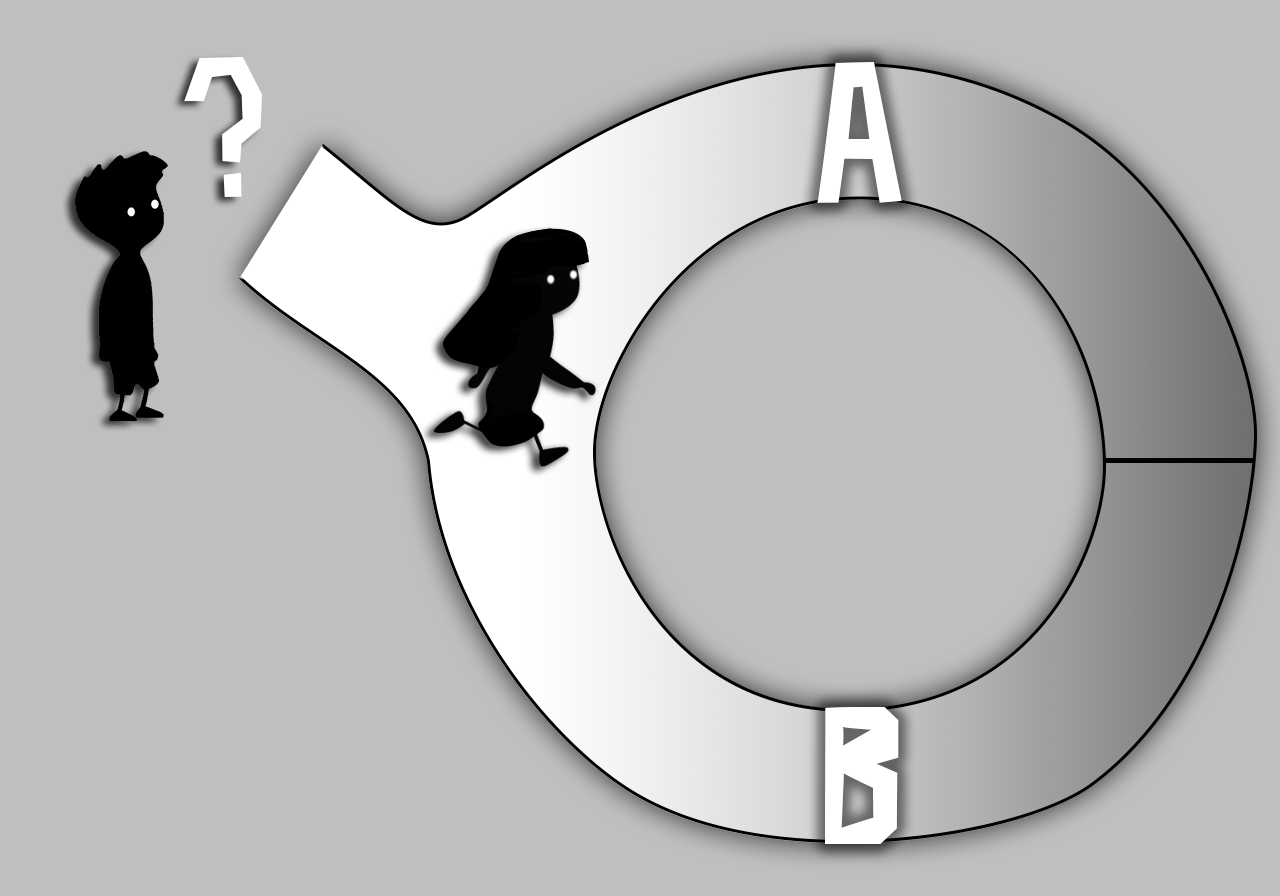
\includegraphics[width=\linewidth]{gfx/graficoJL_ZKP_1}
	\caption*{The cave \citep{ZKPcave:fig}. Peggy takes randomly A or B. Victor awaits outside.}\label{fig:1}
	\endminipage\hfill
	\minipage{0.3\textwidth}
	
\includegraphics[width=\linewidth]{gfx/graficoJL_ZKP_2}
	\caption*{Victor chooses randomly the returning path for Peggy.}\label{fig:2}
	\endminipage\hfill
	\minipage{0.3\textwidth}%
	
\includegraphics[width=\linewidth]{gfx/graficoJL_ZKP_3}
	\caption*{Peggy returns by the requested path.\\ }\label{fig:3}
	\endminipage
\end{figure}



Many different types of problems are used in the formal study of Zero-Knowledge Proofs, in which those related to number theory and graph theory stand out the most. Theses problems are hard to solve for those who don't know any extra information about the problem, in our story the problem would be opening the door without knowing the magic word. 

The most representative problems in Zero-Knowledge Proofs are the discrete logarithm, the square root modulo a composite integer, the graph isomorphism, finding hamiltonian cycles and the 3-colorability of graphs.

The discrete logarithm consists on, given a cyclic group of prime order, a generator $g$ and an element $y$ in that group, finding the power $s$ such that $g^s=y$, that is, the discrete logarithm base $g$ of $y$, $log_g y$.

The problem of the modular square root involves the quadratic residues theory, which shows us that if the modulus is a prime number, it is easy to find the square root, if it exists, of a given value, but if the modulus is composite, and we don't know its factorization in prime factors, it is hard to even tell if a given value is a quadratic residue, that is, it has square roots.

The graph isomorphism problem consists on given two distinct graphs, tell if there exists an isomorphism between them. This problem has many particular cases easy to solve, but the best known algorithm to solve any instance of the problem is only quasi-polynomial in time, and it is still under revision.

A hamiltonian graph is that with a cycle with every node in the graph, without repetitions.

The 3-colorability of a graph consists on giving each pair of connected nodes two different colors, in a way all the nodes in the graph have only one color, and we used exactly 3 colors.

The hamiltonian cycle and 3-colorability problems have in common that both are categorized in the class of problems known as \textbf{NP}-complete. This means that solving one \textbf{NP}-complete problem is equivalent to solve any other, but to this day no efficient algorithm for any of them is known.


We divide this paper in three parts, during the first one we will study all these problems, starting with defining what we understand a \textit{hard} problem actually is, from a computational point of view, then we will formally describe the mentioned problems, as well as the algorithms that, knowing some extra information (the secret), allow us to solve them.

The second part of this memory will focus on the Zero-Knowledge Proofs themselves, defining what properties must have a proof of this kind, and we will state various proofs related to the problems previously described, proving that each one of them satisfy the definition.

We will first define what an interactive proof formally is, so we then can build on top of it the definition of a Zero-Knowledge Proof, which intuitively is interactive. The first kind of Zero-Knowledge Proof is known as perfect, because no machine would be capable of obtaining any extra information from them. Because this particular definition is very constraining, we will relax it in two ways, the first one, by supposing that our verifier is not malicious, that is, while we interact with it, the verifier won't try to extract extra information from us. The last type of Zero-Knowledge Proofs will be those called computational, in which instead of considering a perfect security against any machine, we consider real world machines, limited in time and memory, and in practice it will give us as much security as the perfect Zero-Knowledge Proofs.


The third part will be dedicated to the practical applications of Zero-Knowledge Proofs. The use of these protocols will let us solve problems related to privacy during communications, increasing application's security and functionality.

One of the most important results in this chapter is the non-interactivity of Zero-Knowledge Proofs, through the Fiat-Shamir heuristic, which uses hash functions, hard to predict in the practice.

Combining many techniques of the Zero-Knowledge Proofs, IBM developed a security suite protocol for privacy preserving, called Identity Mixer. The issuance of credentials uses the Camenisch-Lysyanskaya signature, which most strong features are that it can be performed between two parties, and it can be randomized, in a way some values of the signature change affected by a random parameter, but the signature is still valid.

Then, a certificate can be partially disclosed, that is, when a user presents its certificate to a verifier, only part of the certificate is shown, and the other part is committed with a Zero-Knowledge Proof assuring the hidden values are signed by a valid Camenisch-Lysyanskaya signature, which is also randomized to avoid correlations between different uses of the certificate.

%Identity Mixer accomplishes authentication in a real privacy preserving fashion, removing the need of storing delicate information in the server side, avoiding possible security attacks where the user could not say anything about the security measures to apply. \textit{``If your personal data is never collected, it can not be stolen''} -- Maria Dubovitskaya, from the Identity Mixer team.


Finally, we include an appendix to show some implementations of these algorithms using \texttt{sage}, a Python based mathematical software of free distribution. It offers tools for modular arithmetic so we can focus on the implementation of the protocols instead of writing efficient implementations of modular arithmetic operations to work in other programming languages. These implementations are not related to the Computer Science thesis, which uses the C programming language and focuses on other kind of devices.






\end{otherlanguage}

\endgroup			

\vfill
%\cleardoublepage%*******************************************************
% Publications
%*******************************************************
\pdfbookmark[1]{Publications}{publications}
\chapter*{Publications}\graffito{This is just an early --~and currently ugly~-- test!}
This might come in handy for PhD theses: some ideas and figures have appeared previously in the following publications:

%\noindent Put your publications from the thesis here. The packages \texttt{multibib} or \texttt{bibtopic} etc. can be used to handle multiple different bibliographies in your document.

\begin{refsection}[ownpubs]
    \small
    \nocite{*} % is local to to the enclosing refsection
    \printbibliography[heading=none]
\end{refsection}

\emph{Attention}: This requires a separate run of \texttt{bibtex} for your \texttt{refsection}, \eg, \texttt{ClassicThesis1-blx} for this file. You might also use \texttt{biber} as the backend for \texttt{biblatex}. See also \url{http://tex.stackexchange.com/questions/128196/problem-with-refsection}.
%\cleardoublepage%*******************************************************
% Acknowledgments
%*******************************************************
\pdfbookmark[1]{Acknowledgments}{acknowledgments}

\begin{flushright}{\slshape    
    We have seen that computer programming is an art, \\ 
    because it applies accumulated knowledge to the world, \\ 
    because it requires skill and ingenuity, and especially \\
    because it produces objects of beauty.} \\ \medskip
    --- \defcitealias{knuth:1974}{Donald E. Knuth}\citetalias{knuth:1974} \citep{knuth:1974}
\end{flushright}



\bigskip

\begingroup
\let\clearpage\relax
\let\cleardoublepage\relax
\let\cleardoublepage\relax
\chapter*{Acknowledgments}
Put your acknowledgments here.

Many thanks to everybody who already sent me a postcard!

Regarding the typography and other help, many thanks go to Marco 
Kuhlmann, Philipp Lehman, Lothar Schlesier, Jim Young, Lorenzo 
Pantieri and Enrico Gregorio\footnote{Members of GuIT (Gruppo 
Italiano Utilizzatori di \TeX\ e \LaTeX )}, J\"org Sommer, 
Joachim K\"ostler, Daniel Gottschlag, Denis Aydin, Paride 
Legovini, Steffen Prochnow, Nicolas Repp, Hinrich Harms, 
 Roland Winkler, Jörg Weber, Henri Menke, Claus Lahiri, 
 Clemens Niederberger, Stefano Bragaglia, Jörn Hees, 
 and the whole \LaTeX-community for support, ideas and 
 some great software.

\bigskip

\noindent\emph{Regarding \mLyX}: The \mLyX\ port was intially done by 
\emph{Nicholas Mariette} in March 2009 and continued by 
\emph{Ivo Pletikosi\'c} in 2011. Thank you very much for your 
work and for the contributions to the original style.


\endgroup




\pagestyle{scrheadings}
\cleardoublepage%*******************************************************
% Table of Contents
%*******************************************************
%\phantomsection
\refstepcounter{dummy}
\pdfbookmark[1]{\contentsname}{tableofcontents}
\setcounter{tocdepth}{2} % <-- 2 includes up to subsections in the ToC
\setcounter{secnumdepth}{3} % <-- 3 numbers up to subsubsections
\manualmark
\markboth{\spacedlowsmallcaps{\contentsname}}{\spacedlowsmallcaps{\contentsname}}
\tableofcontents 
\automark[section]{chapter}
\renewcommand{\chaptermark}[1]{\markboth{\spacedlowsmallcaps{#1}}{\spacedlowsmallcaps{#1}}}
\renewcommand{\sectionmark}[1]{\markright{\thesection\enspace\spacedlowsmallcaps{#1}}}
%*******************************************************
% List of Figures and of the Tables
%*******************************************************
\clearpage

\begingroup 
    \let\clearpage\relax
    \let\cleardoublepage\relax
    \let\cleardoublepage\relax
    %*******************************************************
    % List of Figures
    %*******************************************************    
    %\phantomsection 
    \refstepcounter{dummy}
    %\addcontentsline{toc}{chapter}{\listfigurename}
    \pdfbookmark[1]{\listfigurename}{lof}
    \listoffigures

    \vspace{8ex}

    %*******************************************************
    % List of Tables
    %*******************************************************
    %\phantomsection 
    \refstepcounter{dummy}
    %\addcontentsline{toc}{chapter}{\listtablename}
    \pdfbookmark[1]{\listtablename}{lot}
    \listoftables
        
    \vspace{8ex}
%   \newpage
    
    %*******************************************************
    % List of Listings
    %*******************************************************      
      %\phantomsection 
    \refstepcounter{dummy}
    %\addcontentsline{toc}{chapter}{\lstlistlistingname}
    \pdfbookmark[1]{\lstlistlistingname}{lol}
    \lstlistoflistings 

    \vspace{8ex}
       
    %*******************************************************
    % Acronyms
    %*******************************************************
    %\phantomsection 
    \refstepcounter{dummy}
    \pdfbookmark[1]{Acronyms}{acronyms}
    \markboth{\spacedlowsmallcaps{Acronyms}}{\spacedlowsmallcaps{Acronyms}}
    \chapter*{Acronyms}
    \begin{acronym}[UMLX]
        \acro{DRY}{Don't Repeat Yourself}
        \acro{API}{Application Programming Interface}
        \acro{UML}{Unified Modeling Language}
    \end{acronym}                     
\endgroup

%********************************************************************
% Mainmatter
%*******************************************************
\cleardoublepage\pagenumbering{arabic}
%\setcounter{page}{90}
% use \cleardoublepage here to avoid problems with pdfbookmark
\cleardoublepage
%************************************************
\chapter{Introducción}\label{ch:introduction}
%************************************************


\cleardoublepage
%*****************************************
\chapter{Preliminares de Computación}\label{ch:preliminaresComputacion}
%*****************************************

% handbook of applied
% apuntes algebra conmutativa


%para relacionar con la criptografía, ver WIKIPEDIA
% https://en.wikipedia.org/wiki/Computational_complexity_theory#Problems_in_NP_not_known_to_be_in_P_or_NP-complete

% Handbook of applied
% Fundamentals of Computer Security
% Apuntes AED II

% Estructura:
% Intro con definiciones de problema, algoritmo, Problemas de decisión
%  Subsección: Notación asintótica, clases de complejidad (polinómico, exponencial, ejemplos)
%  Subsección: Clases P y NP, ___
%  Subsección: Algoritmos probabilísticos, ¿ensembles?, ¿preliminares de estadística?
%  Subsección: El uso en criptografía por la suposición de P!=NP, intractability, nombrar los 3 problemas NPI, y dejar el estudio y por qué son NPI para sus respectivas secciones.


En este capítulo introducimos unos preliminares sobre la complejidad computacional, que nos permitirán entender qué problemas matemáticos, y por qué, se utilizan en criptografía. Comencemos con unas definiciones:

\begin{definition}
	Llamamos \textit{problema} a la descripción general de una tarea que depende de unos parámetros. La \textit{definición} de un problema consta de dos partes. La primera da el escenario del problema, describiendo los parámetros necesarios. La segunda parte indica una pregunta de la que se espera una respuesta o solución.
\end{definition}

\begin{example}
	Vamos a considerar el problema de multiplicar dos matrices. La definición del problema sería:
	
	\begin{tabular}{|ll}
		\textit{Nombre:} & Problema multiplicación de matrices. \\
		\textit{Parámetros:} & Dos matrices $A_1$ y $A_2$. \\
		\textit{Pregunta:} & ¿Cuál es la matriz $A$ tal que $A=A_1 \cdot A_2$? \\
	\end{tabular}
\end{example}

\begin{definition}
	Una \textit{instancia} de un problema es el caso particular de un problema al que se le han dado valores a los parámetros.
\end{definition}


\begin{definition}	
	Un \textit{algoritmo} es una lista de instrucciones que para una instancia produce una respuesta correcta. Se dice que un algoritmo \textit{resuelve} un problema si devuelve respuestas correctas para todas las instancias del problema.
\end{definition}


\begin{definition}
	Se llama \textit{problema de decisión} a un problema cuya respuesta está en el conjunto $\mathcal{B}= \{Verdadero, Falso\}$.
\end{definition}


No todos los problemas son de decisión, pero en general es fácil transformarlos en un problema de decisión cambiando la \textit{pregunta}, y los algoritmos que resuelven un problema de decisión suelen también ser fáciles de adaptar para el problema original.

\begin{example}
	El problema del ejemplo anterior se puede transformar a un problema de decisión:
	
	\begin{tabular}{|ll}
		\textit{Nombre:} & Problema multiplicación de matrices. \\
		\textit{Parámetros:} & Tres matrices $A$, $A_1$ y $A_2$. \\
		\textit{Pregunta:} & ¿$ A = A_1 \cdot A_2$? \\
	\end{tabular}
	\\
	\hfil
	
	Un algoritmo para solucionarlo puede primero comprobar las dimensiones de las matrices, y si no concuerdan con las de la multiplicación, puede responder $Falso$ sin más operaciones, pero cuando las dimensiones concuerden, deberá realizar la multiplicación de $A_1$ por $A_2$ y luego comparar $A$ con el producto obtenido.
	
\end{example}

\hfil

\section{Notación asintótica} 

Para poder estudiar cómo crecen el tiempo de ejecución, la memoria usada, o cualquier otro recurso, de un algoritmo, dependiendo del tamaño de los datos de entrada, utilizamos distintas \textit{notaciones asintóticas}. Nos interesa en particular la siguiente:

\begin{definition}
	Sea $f : \mathbb{N} \rightarrow \mathbb{R}^+$. Definimos la notación \textit{O grande} u \textit{orden} de $f$ al conjunto de funciones de $\mathbb{N}$ a $\mathbb{R}^+$ acotadas superiormente por un múltiplo positivo de $f$ a partir de cierto valor $n \in \mathbb{N}$:
	
	$O(f) = \{t:\mathbb{N} \rightarrow \mathbb{R}^+ \, | \; \exists c \in \mathbb{R}^+,\, \exists 
	n_0\in \mathbb{N} \, : \, t(n) \leq c\cdot f(n) \quad \forall n \geq n_0  \}$. 
	
\end{definition}

\hfil

Para estudiar el tiempo de ejecución, $t : \mathbb{N} \rightarrow \mathbb{R}^+$ (el tiempo promedio, el caso más desfavorable, \dots), de un algoritmo, buscaremos una función $f$ que acote a $t$ lo más de cerca posible. Para ello definimos la relación de orden:

\begin{definition}
	Sean $f, g : \mathbb{N} \rightarrow \mathbb{R}^+$.
	\marginpar{Comparación de órdenes: $ O(1) \leq O(ln\,n) \leq O(\sqrt{n}) \leq O(n) \leq O(n\,ln\,n) \leq O(n^c) \leq O(n^{ln\,n}) \leq O(c^n) \leq O(n!) \leq O(n^n) $, donde $c>1$ constante.}
	Diremos que  $O(f) \leq O(g)$ si $\forall t \in O(f)$ se tiene que $t \in O(g)$, es decir,  $O(f) \subseteq O(g)$.
\end{definition}

Para acotar $t$ buscaremos el menor $O(f) : t\in O(f)$.

% La función $t : \mathbb{N} \rightarrow \mathbb{R}^+$, del tiempo de ejecución de un algoritmo, toma en general como parámetro el tamaño de la entrada. Éste depende de la representación que se le dé a los parámetros, pero podemos pensar siempre en la representación binaria de los números enteros excepto que se indique lo contrario. Esta representación utiliza $1+log_2(n)$ bits para un entero $n$, y podemos simplificar para $n$ suficientemente grande a $log_2(n)$.

\hfil 

\section{Clases de complejidad}

Para estudiar los problemas de decisión los organizamos en clases de complejidad, según sus mejores algoritmos que los solucionan.


\begin{definition}
	Se llama algoritmo de \textit{tiempo de cálculo polinomial} al algoritmo cuya función de tiempo del caso más desfavorable es de orden $O(n^k)$, donde $n$ es el tamaño de la entrada y $k$ una constante. Cualquier algoritmo cuyo tiempo de ejecución no puede acotarse de esa manera se llama de \textit{tiempo de cálculo exponencial}.
\end{definition}

A veces se denominan \textit{buenos} o \textit{eficientes} a los algoritmos polinomiales, e \textit{ineficientes} a los exponenciales. Sin embargo, hay casos particulares donde no ocurre. Lo más importante al tratar con algoritmos polinomiales es el grado del polinomio, $k$, que indica su orden de complejidad. Por ejemplo, consideremos un problema cuyo mejor algoritmo tarda $n^{100}$ instrucciones, es de orden polinómico, pero prácticamente intratable a partir de $n=2$, y por otra parte, un problema que utilice $2^{0.00001n}$ instrucciones podría tratar casos hasta de $n=10^6$ sin dificultad.
Por esto, en criptografía se debe considerar el caso promedio sobre el caso más desfavorable.


\begin{definition}
	El conjunto de problemas de decisión que se pueden resolver en tiempo polinomial se llama clase \textbf{P}.
\end{definition}

\begin{definition}
	\label{def:NP}
	Se llama clase de complejidad \textbf{NP} al conjunto de problemas de decisión donde una respuesta que sea $Verdadero$ se puede verificar en tiempo polinomial, dada cierta información extra, que llamaremos \textit{certificado}.
\end{definition}

\begin{definition}
	Se llama clase de complejidad \textbf{co-NP} al conjunto de problemas de decisión donde una respuesta que sea $Falso$ se puede verificar en tiempo polinomial, dado el correspondiente \textit{certificado}.
\end{definition}

Es inmediato que  que \textbf{P} $\subseteq$ \textbf{NP} y \textbf{P} $\subseteq$ \textbf{co-NP}.

\begin{example}[Problema en \textbf{NP}]
	Consideremos el siguiente problema de decisión:
	
	\begin{tabular}{|ll}
		\textit{Nombre:} & Problema del entero compuesto. \\
		\textit{Parámetros:} & Un entero positivo $n$. \\
		\textit{Pregunta:} & ¿Es $n$ compuesto? Es decir, ¿existen \\
		&  enteros $a$, $b > 1$ tal que $n=ab$? \\
	\end{tabular}
	\\
	
	El problema pertenece a \textbf{NP} porque se puede comprobar en tiempo polinomial que $n$ es compuesto si nos dan su \textit{certificado}, un divisor $a$ de $n$, tal que $1 < a < n$. Basta usar la división euclídea de $n$ entre $a$ y ver que el resto es $0$. Sin embargo, aún no se conoce si pertenece a \textbf{P}.
\end{example}


\hfil

\begin{definition}
	\label{reducePoly:def}
	Sean dos problemas de decisión $L_1, L_2 \in $ \textbf{NP}, con correspondientes conjuntos de instancias $I_1$ e $I_2$. Sean $I_1^+$ e $I_2^+$ los subconjuntos de todas las instancias ``$Verdaderas$'' de $I_1$ e $I_2$, respectivamente. Decimos que $L_1$ es \textit{reducible en tiempo polinomial} a $L_2$, $L_1 \leq_P L_2$, si existe una función $f:I_1 \Rightarrow I_2$ que cumple:
	
	\begin{enumerate}
		\item Es ejecutable en tiempo polinomial.
		\item $x \in I_1^+  \Leftrightarrow  f(x) \in I_2^+ $.
	\end{enumerate}
\end{definition}

\hfil

De manera más informal, se dice que $L_1$ se reduce en tiempo polinomial a $L_2$ si hay un algoritmo que resuelve $L_1$ utilizando como subrutina un algoritmo que resuelve $L_2$, y que se ejecuta en total en tiempo polinomial, si lo hace el algoritmo que resuelve $L_2$.

Si $L_1 \leq_P L_2$, entonces se puede entender que $L_2$ es al menos computacionalmente tan difícil como $L_1$, o que $L_1$ no es más difícil que $L_2$.

\begin{definition}
	Un problema de decisión $L$ se dice que es \textbf{NP}-completo, o \textbf{NPC} si:
	\begin{enumerate}[label=(\roman*)]
		\item $L \in $ \textbf{NP}, y
		\item $L_1 \leq_P L \quad \forall L_1 \in $ \textbf{NP}.
	\end{enumerate}
\end{definition}

\hfil

Los problemas \textbf{NPC} son los más difíciles entre los \textbf{NP} en el sentido de que son al menos tan difíciles como el resto de problemas en \textbf{NP}. Veamos el problema \textbf{NPC} más característico:

\begin{tabular}{|ll}
	\textit{Nombre:} & Problema de satisfacibilidad booleana (SAT). \\
	\textit{Parámetros:} & Una colección finita $C$ de expresiones booleanas \\
	&  con variables y sin cuantificadores. \\
	\textit{Pregunta:} & ¿Hay alguna asignación de las variables que \\ & haga $Verdadero$ a $C$? \\
\end{tabular}
\\

\begin{theorem}[Teorema de Cook (1971)]
	El problema de satisfacibilidad booleana es \textbf{NPC}.
\end{theorem}\marginpar{Para conocer más sobre el problema y la demostración se puede consultar \citep{book:1056906}.}


O expresado de otra manera:

\begin{theorem}
	\label{redNPC:theo}
	Todo problema $Q \in $ \textbf{NP} se puede reducir en tiempo polinomial al problema de satisfacibilidad booleana.
	
	$\forall Q \in $ \textbf{NP}, $Q \leq_P SAT$.
\end{theorem}


\hfil

A día de hoy conocemos ciertas propiedades sobre las clases de equivalencia, pero quedan muchas cuestiones sin resolver:

\begin{itemize}
	\item Uno de los siete problemas del milenio, ¿\textbf{P} $=$ \textbf{NP}?
	\item ¿\textbf{NP} $=$ \textbf{co-NP}?
	\item ¿\textbf{P} $=$ \textbf{NP} $\cap$ \textbf{co-NP}?
\end{itemize}


La opinión de los expertos en base a ciertas evidencias es que la respuesta a las tres es \textit{no}, pero hasta que se encuentren demostraciones formales de cada una, quedarán en conjeturas. Y basándose en esas conjeturas es donde se apoya la seguridad informática.


\begin{figure}[bth]
	\begin{center}
		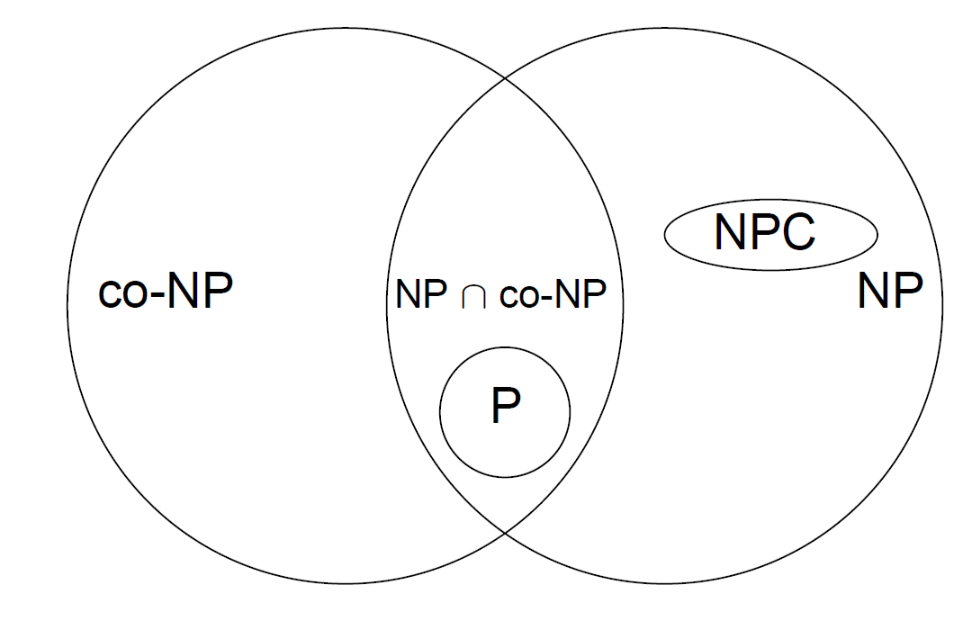
\includegraphics[width=.45\linewidth]{gfx/NPclasses}
	\end{center}
	\caption{Conjetura de las relaciones entre clases \textbf{NP}, \textbf{co-NP}, \textbf{NPC}, \textbf{P}.}
	\label{fig:NPclasses}
\end{figure}


Existen tres problemas que se conoce que pertenecen a \textbf{NP}, pero se desconoce a día de hoy si pertenecen a \textbf{P} o \textbf{NPC}: el isomorfismo de grafos, el logaritmo discreto y la factorización de enteros.

En los siguientes capítulos los estudiaremos como base de diferentes pruebas de conocimiento cero.


\hfil


\section{Algoritmos probabilísticos} 

\hfil

Para intentar resolver la infactibilidad computacional de ciertos problemas, surge un modelo alternativo de computación que utiliza métodos probabilísticos. Estos métodos no pueden asegurar cotas superiores absolutas de tiempo, e incluso pueden devolver una respuesta errónea. Sin embargo, dadas unas cotas muy pequeñas de errores, en la práctica, ciertos métodos probabilísticos son más eficientes que los algoritmos conocidos, pues el tiempo de ejecución \textit{esperado} del método, calculado probabilísticamente, es menor que el orden del algoritmo original.


% Tipos de algoritmos probabilísticos según errores
% Ejemplo de test de primalidad

\begin{definition}
	Llamamos \textit{algoritmo de Monte Carlo} a un algoritmo probabilístico que resuelve un problema de decisión, pero tiene un error $\epsilon$ de equivocarse.
	
	Decimos que es \textit{parcialmente} $Verdadero$ si cuando se le da una instancia $Verdadera$ nunca se equivoca, pero si la instancia es $Falsa$ puede devolver $Verdadero$ con probabilidad $\epsilon$. De la misma manera, decimos que es \textit{parcialmente} $Falso$ si siempre resuelve correctamente instancias $Falsas$, pero puede cometer un error al resolver instancias $Verdaderas$.
\end{definition}


\begin{definition}
	Llamamos \textit{algoritmo de Las Vegas} a un algoritmo probabilístico que resuelve un problema de decisión, pero o bien lo resuelve correctamente, o bien informa de error y termina sin resolver el problema con una probabilidad $\epsilon$.
\end{definition}



\begin{example}[Test de primalidad]
	El problema de decisión
	
	\begin{tabular}{|ll}
		\textit{Nombre:} & Problema de primalidad (PRIM). \\
		\textit{Parámetros:} & Un entero $n$. \\
		\textit{Pregunta:} & ¿Es $n$ primo? \\
	\end{tabular}
	\\
	\hfil
	
	es un problema en \textbf{NP}$\cap$\textbf{co-NP} (es el contrario del problema del entero compuesto), pero no se conoce ningún algoritmo que lo resuelva en tiempo polinómico, por ello no sabemos aún si pertenece a \textbf{P}.
	
	Un algoritmo probabilístico basado en el Pequeño Teorema de Fermat, $a^{n-1} \equiv 1 \, mod \, n$ si $n$ es primo para cualquier $a\in \mathbb{Z}_n$, puede utilizarse para comprobar si $n$ es primo.
	
	Si $n$ es primo, para todo $a$ que se elija, se cumplirá $a^{n-1} \equiv 1 \, mod \, n$, por lo que es un algoritmo de Monte Carlo parcialmente $Verdadero$, para una instancia $Verdadera$ nunca se equivoca.
	
	Sin embargo, si $n$ es compuesto, pueden existir valores $a$ que cumplan la propiedad. Por ejemplo, si $n$ es un \textit{número de Carmichael}, todo $a$ coprimo con $n$ cumple $a^{n-1} \equiv 1 \, mod \, n$.
	
	Este no es el test de primalidad más fuerte, existen otros mejorados, como el test de primalidad de Miller-Rabin, que asegura que a lo sumo da un falso positivo para $\frac{1}{4}$ de todos los enteros $a$, $0<a\leq p-1$. Ejecutando el test un número $k$ de veces, eligiendo aleatoriamente $a\in \mathbb{Z}_n$, obtenemos una probabilidad de error de $\epsilon=\frac{1}{4^k}$, lo que podría darnos en 50 iteraciones un algoritmo ejecutable en tiempo polinomial, con probabilidad de error, cuando $n$ es compuesto, de $2^{-50}$, algo que podemos estar dispuestos a asumir en la práctica.
	
\end{example}


\cleardoublepage
%*****************************************
\chapter{Problemas Basados en Grafos}\label{ch:preliminaresGrafos}
%*****************************************

\section{Introducci\'on a la Teoría de Grafos}

\begin{definition}
	Un \textit{grafo} (simple no dirigido) es un par $(V,E)$ formado por un conjunto
	finito $V \neq \emptyset$, a cuyos elementos denominaremos \textit{vértices} o
	\textit{nodos}, y $E$, un conjunto de pares (no ordenados y formados por distintos
	vértices) de elementos de $V$, a los que llamaremos \textit{aristas}.

	A los nodos $v_1$ y $v_2$ que forman una arista $e = (v_1, v_2)$ se les llama
	\textit{extremos} de $e$.
\end{definition}


\begin{definition}[Conceptos]
	\begin{itemize}
	\item A dos nodos $v_1$ y $v_2$ que forman parte de una misma arista se les llama \textit{adyacentes}.
  \item Se dice que una arista es \textit{incidente} con un vértice $v$ cuando $v$ es uno de sus extremos.
	\item El grado de un nodo $v \in V$ es el n\'umero de aristas incidentes en \'el.
  \item Un camino es una sucesi\'on de nodos $(v_1,v_2,\cdots,v_k)$ tales que
	para todo $i \in \{1,\cdots,k-1\}$ se tiene que $(v_i,v_{i+1}) \in V$.
	\item La longitud de un camino se define como el n\'umero de aristas que lo forman,
	en el caso del camino $(v_1,v_2,\cdots,v_k)$ la longitud es $k-1$.
	\item Un camino $(v_1,v_2,\cdots,v_k)$ se dir\'a un ciclo si $v_1 = v_k$ y no
	se repite ning\'un otro nodo del grafo, es decir, para todo $i,j \in
	\{1,\cdots,k-1\}$, si $i\not= j$ entonces $v_i \not= v_j$.
	\item Un ciclo $(v_1,v_2,\cdots,v_k)$ se dir\'a un ciclo hamiltoniano si contiene
	a todos los nodos.
	\item Un grafo diremos que es hamiltoniano si tiene un ciclo hamiltoniano.
\end{itemize}
\end{definition}

\begin{definition}
	Dos grafos $G_1 = (V_1, E_1)$ y $G_2 = (V_2, E_2)$ se dice que son \textit{isomorfos},
	lo cual denotaremos como $G_1 \simeq G_2$, si existe una aplicación biyectiva
	$\tau : V_1 \rightarrow V_2$ tal que $\forall u,v \in V_1$
	$(u,v) \in E_1 \Leftrightarrow (\tau(u), \tau(v)) \in E_2 $.
	Tal aplicación recibe el nombre de \textit{isomorfismo}.
\end{definition}

\begin{proposition}
Dados dos grafos isomorfos $G_1 = (V_1,E_1)$ y $G_2 = (V_2,E_2)$, entonces $G_1$
tiene un ciclo hamiltoniano si y s\'olo si $G_2$ tiene un ciclo hamiltoniano. Es
decir, la propiedad de ser un grafo hamiltoniano se conserva por isomorfismos.
\end{proposition}
\begin{proof}
Sea $\tau : V_1 \to V_2$ el isomorfismo y sea $(v_1,v_2,\cdots,v_k)$ el ciclo
hamiltoniano de $V_1$. Entonces $(\tau(v_1),\tau(v_2),\cdots,\tau(v_k))$ el el
ciclo hamiltoniano de $G_2$ ya que, por un lado es un ciclo puesto que
$(v_i,v_{i+1}) \in E_1$ implica que $(\tau(v_i),\tau(v_{i+1}))\in E_2$,
y por otro, al ser $\tau$ biyectiva, el ciclo contiene a todos los nodos
sin repetir ninguno (salvo los extremos).
\end{proof}

\begin{definition}
	Una \textit{coloración} de un grafo $G=(V,E)$ es una aplicación $c:V\rightarrow
	\{1,2,\dots , l\}$. El valor $c(v_i)$ es el \textit{color} correspondiente al
	nodo $v_i$.
\end{definition}

\begin{definition}
	Una \textit{coloración propia} de un grafo es una coloración que hace corresponder
	colores diferentes a vértices adyacentes, es decir
	$\forall (u,v)\in E$ se tiene que $c(u)\neq c(v)$.
\end{definition}


\begin{definition}
	Llamaremos \textit{número cromático} del grafo $G$, $\chi(G)$, al mínimo valor
	de $l$ que permite una coloración propia de $G$, es decir, al mínimo número de
	colores necesarios para colorear los vértices de forma que los extremos de cada
	arista tengan colores distintos.
\end{definition}

En las siguientes secciones de este cap\'itulo,
introducimos los enunciados de los problemas de grafos
utilizados en pruebas de conocimiento cero.

\section{El Problema del Isomorfismo de Grafos}

\hfil

\begin{tabular}{|ll}
	\textit{Nombre:} & Problema GI ({\em Graph Isomorphism}). \\
	\textit{Parámetros:} & Dos grafos $G_1 = (V_1, E_1)$ y $G_2 = (V_2, E_2)$,
	\\ & del mismo orden $\mid V_1 \mid = \mid V_2 \mid = n$. \\
	\textit{Pregunta:} & ¿Existe un isomorfismo $\tau : V_1 \rightarrow V_2$
	tal que \\ & una arista $(u,v)\in E_1$ si y solo si $(\tau (u),\tau (v))
	\in E_2$? \\
\end{tabular}
\\

\hfil

Una forma de tratar este problema por fuerza bruta consistir\'ia en calcular
todas las posibles premutaciones de $n$ elementos para ver si una de ellas
cumple las concidiones requeridas para el isomorfismo de grafos. Puesto que el
n\'umero de permutaciones de $n$ elementos es $n!$, esta aproximaci\'on ser\'ia
claramente polin\'omica e intratable para valores de $n$ m\'inimamente grandes.

Sin embargo, el problema puede tener casos en los cuales la soluci\'on sea
relativamente sencilla ya que los isomorfismos de grafos conservan muchas de las
propiedades del grafo. Por ejemplo, podemos calcular de forma muy r\'apida los
grados de todos los nodos y dado un isomorfismo $\tau$ tenemos que el grado de
$u$ es siempre el mismo que el grado de $\tau(u)$ para cualquier nodo $u$.

Esto nos puede restringir el problema a las permutaciones que se puedan construir
manteniendo los grados. Es algo parecido a lo que sucede con el algoritmo de la factorizaci\'on de enteros,
que en casos particulares puede tener una soluci\'on sencilla, pero debemos considerar
el caso peor para la utilizaci\'on de este problema como base de la seguridad de otros algoritmos.

El problema del isomorfismo de grafos se sabe desde hace tiempo que no es puramente
exponencial y que existen cotas subexponenciales, diferentes para algunos casos particulares,
pero ciertamente mejores que la exponencial.

Muy recientemente se han producido novedades en relaci\'on con este problema. Concretamente
en el a\~no 2015 el profesor László Babai present\'o un algoritmo quasi-polin\'omico para
el problema del isomorfismo de grafos. Esta publicaci\'on se puede consultar por ejemplo en \cite{babai}.
Sin embargo el 4 de enero de 2017, el propio autor se retractaba de su propio resultado al haber sido
detectado un error en la demostraci\'on. Poco despu\'es, el 9 de enero de 2017, anunciaba una versi\'on
corregida del problema que parece que se ha confirmado como correcta.

La complejidad que presenta este algoritmo es $e^{(\ln n)^{O(1)}}$. Las consecuencias que esto puede
tener en la utilizaci\'on del problema del isomorfismo de grafos en algoritmos de seguridad criptogr\'afica
es algo que escapa a nuestros conocimientos aunque no parece que se haya producido ninguna reacci\'on
importante en relaci\'on con este resultado. En cualquier caso, conviene estar atentos a los avances
en este sentido por si es conveniente usar t\'ecnicas alternativas.

La historia de este descubrimiento se puede consultar en la revista Investigaci\'on y Ciencia,
edici\'on espa\~nola de la
revista Scientific American que est\'a disponible online en
\url{http://www.investigacionyciencia.es/noticias/resuelto-el-problema-del-isomorfismo-de-grafos-otra-vez-14910}.

\hfil

\section{El Problema del Ciclo Hamiltoniano}

\hfil

\begin{tabular}{|ll}
	\textit{Nombre:} & Problema HC ({\em Hamiltonial Cycle}). \\
	\textit{Parámetros:} & Un grafo $G=(V,E)$. \\
	\textit{Pregunta:} & ¿Existe un ciclo hamiltoniano en G? \\
\end{tabular}
\\

\hfil

De nuevo nos encontramos con un problema que podemos resolver considerando todas
las permutaciones de los nodos, ya que si existe una de ellas que nos proporcione
un ciclo hamiltoniano, habr\'iamos resuelto el problema. Pero este algoritmo es
claramente ineficiente puesto que requiere un an\'alisis de $n!$ permutaciones de los
$n$ nodos.

Una forma algo m\'as inteligente ser\'ia partir de un nodo cualquiera y crear una rama con cada uno de los nodos
adyacentes. Para cada uno de ellos, tratamos de expandir de nuevo con todos los nodos adyacentes siempre que
no repitamos el nodo. De esta forma podr\'iamos recorrer todas las opciones, pero volvemos a
encontrar un n\'umero de casos exponencial.

Este problema, sin embargo, est\'a en una situaci\'on muy distinta del problema anterior,
de hecho, el problema del ciclo hamiltoniano es un problema ${\bf NPC}$ por lo que si existiera un algoritmo
polin\'omico para resolverlo, tendr\'iamos que ${\bf P} = {\bf NP}$ y se habr\'ia resuelto uno de los problemas
del milenio.

La demostraci\'on de que este problema es ${\bf NPC}$ se puede ver en
\cite[Section 34.5.3]{algoBB}. El valor que nos sirve de certificado o testigo es precisamente el ciclo hamiltoniano, puesto que
comprobar que un ciclo concreto cumple las condiciones de ciclo hamiltoniano es trivial desde el punto de vista computacional.

\section{El Problema de la 3-coloración}

\hfil

\begin{tabular}{|ll}
	\textit{Nombre:} & Problema G3C. \\
	\textit{Parámetros:} &Un grafo $G=(V,E)$. \\
	\textit{Pregunta:} & ¿Existe una función
	$c : V \to \{1,2,3\}$ tal que \\ & $\forall (u,v)\in E$, se cumple $c(u)\neq c(v)$? \\
\end{tabular}
\\

\hfil

Determinar si un grafo puede tener una coloraci\'on dada por dos colores es
computacionalmente muy sencillo, puesto que no tenemos
mas que dar un color cualquiera al primer nodo, por ejemplo $1$, y todos los
que est\'en conectados con \'el le asignaremos el color $2$.
Ahora tomamos todos los nodos con el color $2$ y para cada uno de los nodos
adyacentes asignamos el color $1$. Si el grafo se puede colorear
con dos colores, este procedimiento nos ir\'a coloreando cada trozo del grafo
(en caso de que haya zonas desconectadas, cada vez que terminemos de colorear una zona,
tendremos que  partir aleatoriamente de nuevo de uno de los nodos de una nueva
zona para extender la coloraci\'on). Si el grafo no se puede colorear con dos colores
llegaremos necesariamente a un nodo coloreado con un color que est\'a unido con
otro del mismo color, en cuyo caso podemos responder
que el grafo necesita m\'as de dos colores para obtener una coloraci\'on.

Dado un grafo, este algoritmo nos responde de forma eficiente al problema de
si se puede colorear con dos colores, o bien devolviendo una coloraci\'on, o bien
diciendo que dicha coloraci\'on es imposible.

El problema es totalmente diferente en el caso de que dispongamos de tres colores.
Dado un nodo cualquiera con un color asignado, por ejemplo $1$, nos da dos opciones
para la coloraci\'on de los nodos adyacentes, o bien $2$ o bien $3$. Podemos tratar
de probar todas las opciones, con lo que obtendr\'iamos un gran n\'umero de opciones
cuando tratamos con un caso gen\'erico (por supuesto casos particulares pueden tener
soluciones sencillas).

De hecho es conocido que este problema tambi\'en pertenece a la clase {\bf NPC}. Una coloraci\'on
concreta usando $3$ colores servir\'ia de certificado de que la respuesta puede ser afirmativa puesto
que commprobar que todas las aristas tienen extremos con colores diferentes es sencillo
computacionalmente, sin embargo, encontrar la coloraci\'on requiere algoritmos exponenciales.

Una demostraci\'on de que el problema de la 3-coloraci\'on es {\bf NPC} se puede encontrar
en \cite[Problem 34-3]{algoBB}.

\hfil

\cleardoublepage
%*****************************************
\chapter{Problemas Basados en Teor\'ia de N\'umeros}\label{ch:preliminaresAlgebra}
%*****************************************

% Sin demostraciones, solo resultados que se necesiten para secciones posteriores

%Para poder comprender los resultados de los siguientes capítulos necesitaremos recordar ciertas definiciones y propiedades de álgebra y grafos que se cursan durante el grado, e introducir otros preliminares de computación que formalizarán el estudio. No incluiremos demostraciones, pues son conceptos básicos de donde partiremos para desarrollar el resto del trabajo, pero el lector que quiera conocerlas puede consultar las referencias en \textbf{TODO: cite} \citep{gruposYanillos}.
% Mejorar párrafo de las referencias e incluir que para probabilidad el cap de intro de JL... y elementos de Zoroa

% handbook of applied
% apuntes algebra conmutativa


%https://en.wikipedia.org/wiki/Schnorr_group

En este cap\'itulo vamos a hacer un repaso de las cuestiones b\'asicas de
aritm\'etica entera y modular en las que se basan los problemas utilizados
para las pruebas de conocimiento cero que estudiaremos en los siguientes
cap\'itulos.

Aunque para muchos de estos problemas se han desarrollado t\'ecnicas muy
avanzadas, como por ejemplo para la factorizaci\'on de enteros o para el
problema del logaritmo discreto, son en general problemas sencillos de
plantear desde el punto de vista matem\'atico y resolubles de forma
eficiente cuando se dispone de informaci\'on adicional, es decir, del
secreto.

Llamar a estos problemas {\em Teor\'ia de N\'umeros} podr\'ia considerarse
excesivo, podr\'iamos simplemente llamarlos problemas artim\'eticos, pero
hemos preferido la terminolog\'ia de {\em Teor\'ia de N\'umeros} para ser
coherentes con muchos textos que incluyen estos m\'etodos dentro del
ep\'igrafe de {\em Introducci\'on a la Teor\'ia de N\'umeros}.

\section{Aritm\'etica Entera y Modular}

Vamos a recordar los conceptos más básicos de la teoría de grupos,
empezando con la definición de operación binaria:

\begin{definition}
Una \textit{operación binaria} en un conjunto $A$ es una aplicación
$\circ : A\times A \rightarrow A$.
\end{definition}

Según una operación binaria cumpla ciertas propiedades, diremos que:

\begin{itemize}
	\item La operación es \textit{asociativa} si $a\circ (b\circ c) =
(a\circ b)\circ c \quad \forall a,b,c\in A$.
	\item La operación es \textit{conmutativa} si $a\circ b=b\circ a
\quad \forall a,b\in A$.
	\item El elemento $e\in A$ es un \textit{elemento neutro} para
$\circ $ si $a\circ e = e\circ a = a \quad \forall a\in A$.
	\item Cuando existe el neutro $e$, el elemento
$b$ es el \textit{inverso} de $a$ si $a\circ b=b\circ a=e$.
\end{itemize}

Podemos ahora dar formalmente la definición de grupo:

\begin{definition}
	Un \textit{grupo} es un conjunto $G$ con una operación asociativa,
con elemento neutro y con inverso para cada elemento. Si la operación es
además conmutativa, se dice que $G$ es un \textit{grupo abeliano}.
\end{definition}

Existen dos notaciones fundamentales para la representaci\'on de los grupos, que
son la notaci\'on aditiva (la operaci\'on de grupo se denota $+$, el elemento
neutro se denota como $0$ y el inverso de $a$ se denota $-a$) y la notaci\'on
multiplicativa (la operaci\'on de grupo se denota $\cdot$, el elemento neutro
se denota como $1$ y el inverso de $a$ se denota $a^{-1}$).
Es habitual utilizar la notaci\'on aditiva para grupos conmutativos y la
multiplicativa para los no conmutativos. Todos los grupos que vamos a tratar en
los problemas relacionados con la Teor\'ia de N\'umeros
ser\'an conmutativos, pero utilizaremos la notaci\'on
aditiva o multiplicativa seg\'un resulte m\'as natural una u otra.


Con la operación suma $+$ habitual, los conjuntos $\mathbb{Z}$, $\mathbb{Q}$ y
$\mathbb{R}$ son grupos abelianos aditivos.

\begin{definition}
Sea $G$ un grupo conmutativo finito y $g \in G$. Llamaremos orden de $g$ y lo denotaremos
$ord(g)$ al menor entero $t$ positivo tal que $g^t = 1$.
\end{definition}

\begin{proposition}
\label{propLagrange1}
Sea $G$ un grupo conmutativo finito con $n$ elementos, entonces para todo
$g \in G$ se tiene que $g^n = 1$.
\end{proposition}
\begin{proof}
Sean $g_1,g_2,\cdots,g_n$ los elementos de $G$. Est\'a claro que si $g_i \not= g_j$ entonces $gg_i \not= gg_j$ puesto que si fueran iguales tendr\'iamos que $g_i = g^{-1}gg_i = g^{-1}gg_j = g_j$, lo cual es una contradicci\'on.
Esto nos garantiza que el conjunto $\{gg_1,gg_2,\cdots,gg_n\}$ tiene que tener $n$ elementos y por lo tanto ser todo $G$, es decir, que como conjuntos tenemos que
$\{g_1,g_2,\cdots,g_n\} = \{gg_1,gg_2,\cdots,gg_n\}$ puesto que solo hay una reordenaci\'on. Como el producto es conmutativo, si multiplicamos todos los elementos tenemos que
$g_1g_2\cdots g_n = g^n g_1g_2\cdots g_n$ y multiplicando por el inverso de $g_1g_2\cdots g_n$ obtenemos el resultado que buscamos.
\end{proof}

Este resultado es tambi\'en cierto para grupos no conmutativos, pero la demostraci\'on no es tan elemental como en este caso, que es el que vamos a necesitar en esta memoria, por
eso hemos hecho una demostraci\'on directa. Esta proposici\'on nos garantiza que el orden de un elemento en un grupo finito tiene que ser menor o igual que el n\'umero de elementos del grupo.

\begin{definition}
Un grupo abeliano finito $G$ diremos que es c\'iclico cuando exista alg\'un elemento
$g$ tal que $ord(g) = |G|$. En caso de existir, un elemento $g$ que cumpla dichas
propiedades se llamar\'a un generador del grupo $G$.
\end{definition}

\hfil

\begin{definition}
	Un \textit{anillo} es un conjunto $A$ con dos operaciones, $+$ y $\cdot$ (suma y producto), tales que:
	\begin{itemize}
		\item $(A,+)$ es un grupo abeliano con elemento neutro $0$.
		\item El producto es asociativo y tiene elemento neutro que
se denota por $1$. Este elemento consideraremos que es distinto del neutro aditivo ($1\neq 0$).
		\item El producto es distributivo con respecto a la suma, es decir,
$\forall a,b,c \in A$ se tiene $a\cdot(b+c)=a\cdot b + a\cdot c$ y $(b+c)\cdot a = b\cdot a + c\cdot a$.
	\end{itemize}

El anillo es \textit{conmutativo} si lo es el producto. En general, no todos los
elementos de un anillo son invertibles (es decir, tienen inverso para la multiplicaci\'on),
por ejemplo el elemento $0$ nunca lo es. Un anillo conmutativo donde todo elemento
distinto de cero es invertible, se dice que es un \textit{cuerpo}.
\end{definition}

\begin{definition}
Sea $A$ un anillo conmutativo, $A^*$ denotará el
{\em conjunto de los elementos invertibles en A}. Así, con la
multiplicación usual $\mathbb{Z}^* = \{-1,1\}$.

Los elementos invertibles tambi\'en los llamaremos {\em unidades} del anillo $A$.

Si $A$ es un cuerpo, por definici\'on $A^* = A \setminus \{0\}$, por ejemplo
${\mathbb Q}^* = {\mathbb Q} \setminus \{0\}$ ó ${\mathbb R}^* = {\mathbb R}\setminus \{0\}$.
\end{definition}

\begin{proposition}
El conjunto de las unidades de un anillo conmutativo $A$ forma un grupo
conmutativo con la multiplicaci\'on.
\end{proposition}
\begin{proof}
La multiplicaci\'on de dos unidades $a,b \in A^*$ es una unidad puesto que
si $c$ es inverso de $a$ y $d$ inverso de $b$, $(ab)(dc) = a(bd)c = a\cdot
1\cdot c = ac = 1$. La operaci\'on de multiplicaci\'on es asociativa y
conmutativa por serlo en $A$, el $1$ est\'a en $A$ y todo elemento tiene inverso por
definici\'on de $A^*$.
\end{proof}

\begin{definition}
Sean $A$ y $B$ dos anillos conmutativos y $f:A \to B$ una aplicaci\'on.
Diremos que es un homomorfismo de anillos si $f(a_1 + a_2) = f(a_1) +
f(a_2)$, $f(a_1 a_2) = f(a_1) f(a_2)$, $f(0) = 0$ y $f(1) = 1$. Si la
aplicaci\'on $f$ es biyectiva diremos que $f$ es un isomorfismo y que los
anillos $A$ y $B$ son isomorfos.
\end{definition}

\begin{proposition}
Sea $f:A \to B$ un isomorfismo de anillos conmutativos. Entonces para todo
elemento invertible $a$ de $A$, $f(a)$ es un elemento invertible de $B$, la
aplicaci\'on $f$ restringida a los conjuntos $A^*$ y $B^*$ es un isomorfismo
de grupos abelianos.
\end{proposition}
\begin{proof}
Si $a$ es invertible con inverso $c$ tenemos que $1 = f(1) = f(ac) =
f(a)f(c)$ por lo que $f(c)$ es inverso de $f(a)$ y por lo tanto $f(a) \in
B^*$. Por otro lado, si $b$ es un elemento invertible de $B$ con inverso
$d$, al ser $f$ biyectiva podemos encontrar unos valores $a$ y $c$ \'unicos
tales que $f(a) = b$ y $f(c) = d$, por lo tanto $f(ac) = f(a)f(c) = bd = 1 =
f(1)$, pero al ser $f$ biyectiva deducimos que $ab = 1$ y por lo tanto $f$
es suprayectiva considerada como aplicaci\'on entre $A^*$ y $B^*$. Eso
prueba que la restricci\'on de $f$ es un isomorfismo de grupos abelianos puesto que
evidentemente conserva el producto y el elemento neutro al conservarlo $f$.
\end{proof}

\begin{definition}
Sean $A$ y $B$ dos anillos conmutativos, denotaremos $A \times B$ al anillo
cuyos elementos son los pares ordenados $(a,b)$ con $a \in A$ y $b \in B$,
junto con la suma y el producto componente a componente. El elemento neutro
para la suma en $A \times B$ ser\'a $(0,0)$ y para el producto $(1,1)$.
\end{definition}

\begin{proposition}
Sean $A$ y $B$ dos anillos conmutativos, entonces $(A\times B)^*$ es el
subconjunto de $A \times B$ formado por los pares $A^* \times B^*$.
\end{proposition}
\begin{proof}
Si $a$ es invertible con inverso $c$ y $b$ es invertible con inverso $d$
entonces $(a,b)\cdot(c,d) = (ac,bd) = (1,1)$. Rec\'iprocamente si $(a,b)$ es
un elemento invertible de $A \times B$ tenemos un elemento $(c,d)$ tal que
$(a,b)\cdot(c,d) = (1,1)$, pero eso implica que $ac = 1$ y $bd = 1$ por lo
que $a \in A^*$ y $b \in B^*$.
\end{proof}

\hfil

\begin{definition}
Un entero $d$ se dice un {\em divisor} de un entero $a$ si existe un entero $c$ tal
que $dc = a$. Tambi\'en se dice que $d$ divide a $a$ o que $a$ es un m\'ultiplo
de $d$.
\end{definition}

\begin{definition}
Dados dos enteros $a$ y $b$ y otro entero $n>1$, diremos que $a$ y $b$ son {\bf
congruentes m\'odulo $n$} si $a-b$ es un m\'ultiplo de $n$. Esta relaci\'on se
denotar\'a por $a \equiv b ~(mod~n)$ o simplemente $a \equiv b~mod~n$.
\end{definition}

La relaci\'on de congruencia m\'odulo $n$ es una relaci\'on de equivalencia que
divide al conjunto de los n\'umeros enteros en $n$ clases de equivalencia
distintas. Al conjunto cociente formado por estas clases de equivalencia
se denotar\'a ${\mathbb Z}_n$.

Una posible elecci\'on de representantes para las clases de
equivalencia m\'odulo $n$ son los valores $\{0,1,2,\cdots,n-1\}$.
Si fijamos este conjunto de representantes denotaremos
$- ~ mod ~ n : {\mathbb Z} \to \{0,1,\cdots,n-1\} $
a la aplicaci\'on que dado un elemento $a \in {\mathbb Z}$ nos da el representante
de su clase de equivalencia m\'odulo $n$, lo llamaremos el reducido m\'odulo $n$
de $a$.

Es habitual utilizar los valores $\{0,1,2,\cdots,n-1\}$ para representar tambi\'en
las clases de equivalencia de ${\mathbb Z}_n$, por lo tanto podemos decir $3 \in {\mathbb Z}_7$
para referirnos a la clase de equivalencia del $3$ en el conjunto cociente ${\mathbb Z}_n$.
Esto en general simplifica las notaciones y no causa problemas de interpretaci\'on.

La utilizaci\'on de $-~mod~n$ como un operador entre ${\mathbb Z}$ y $\{0,1,\cdots,n-1\}$
no es del todo est\'andar, pero la utilizaremos en esta memoria porque resulta c\'omoda
para trabajar en aritm\'etica modular y en la pr\'actica, casi todos los lenguajes de
programaci\'on tienen el reducido m\'odulo $n$ como una funci\'on m\'as.

Si $a \equiv b ~(mod~n)$ entonces para cualquier $c \in {\mathbb Z}$ tenemos que
$a + c \equiv b + c ~(mod~n)$ (porque $(b+c)-(a+c) = b-a$ que es un m\'ultiplo de $n$)
y tambi\'en $ac \equiv bc ~(mod~n)$ (porque $bc-ac=(b-a)c$ que es un m\'ultiplo de
$n$ por serlo $b-a$). Esta propiedad nos permite probar que si $a \equiv b~(mod~n)$
y $c \equiv d~(mod~n)$ entonces $a+c \equiv b+c \equiv b+d ~(mod~n)$ y tambi\'en
$ac \equiv bc \equiv bd~(mod~n)$.

Dicho de otra forma, la relaci\'on de congruencia m\'odulo $n$ respeta la suma y el
producto por lo que podemos dotar a ${\mathbb Z}_n$ de estructura de anillo con la
estructura heredada de ${\mathbb Z}$, es decir, dadas dos clases $a$ y $b$, la suma
$a+b$ es la clase de la suma de cualquier representante de $a$ y cualquier
representante de $b$, siendo esta definici\'on independiente del representante
elegido puesto que la congruencia respeta la suma. Lo mismo sucede con el producto,
el producto de las clases, es la clase del producto de dos representantes
cualesquiera de las clases.

Esta definici\'on se simplifica mucho en la pr\'actica
cuando tenemos elegidos unos representantes de las clases y un operador como $~mod~n$
puesto que podemos partir del conjunto $\{0,1,\cdots,n-1\}$, hacer las operaciones de suma
y producto con esos representante y si el resultado final se sale fuera del conjunto de
representantes, aplicar el operador $~mod~n$ al resultado. De esta forma podemos decir
que en el anillo ${\mathbb Z}_2$ se tiene que $1+1=0$ puesto que $1+1$ ser\'ia $2$
pero al aplicar el operador $~mod~2$ obtenemos el resultado $0$.

Para prodecer de esta forma, es fundamental tener un m\'etodo para calcular el reducido
m\'odulo $n$ de cualquier n\'umero, pero eso nos lo va a proporcionar precisamente el
algoritmo de la divisi\'on.

\begin{proposition}
Sean $a,n$ dos n\'umeros enteros con $n > 1$, $q = \lfloor \frac{a}{n} \rfloor$,
entonces $a~mod~n = a-nq$. Estos valores $q$ y $a~mod~n$ son precisamente el
cociente y resto de la divisi\'on entre $a$ y $n$.
\end{proposition}
\begin{proof}
Por definici\'on de $q = \lfloor \frac{a}{n} \rfloor$ sabemos que $q$ es el mayor entero
menor o igual que $\frac{a}{n}$, por lo tanto $q \leq \frac{a}{n} < q+1$ y de ah\'i se
deduce que $qn \leq a < nq+n$ por lo que $0 \leq a-nq < n$, es decir, que el entero
$a-nq$ est\'a en el conjunto $\{0,1,\cdots,n-1\}$ tal y como hab\'iamos exigido a
$a~mod~n$. Adem\'as, con esta definici\'on $a-(a~mod~n) = nq$ por lo que
$a \equiv a~mod~n$.
\end{proof}

\begin{definition}
Dados dos enteros $a$ y $b$, llamaremos m\'aximo com\'un divisor de dichos n\'umeros
(y lo denotaremos $mcd(a,b)$)
al mayor entero no negativo $d$ tal que $d$ divide al mismo tiempo a $a$ y a $b$. Este
n\'umero siempre existe puesto que $1$ es siempre divisor de ambos, por lo que el conjunto
de los divisores comunes no es nunca vac\'io. En el caso particular en que este sea el
\'unico divisor com\'un diremos que $a$ y $b$ son coprimos.
\end{definition}

Para el c\'alculo del m\'aximo com\'un divisor de dos n\'umeros, es muy \'util el
siguiente resultado:

\begin{lemma}
Sean $a$ y $b$ dos enteros positivos. Entonces el conjunto de divisores comunes de
$a$ y $b$ es el mismo que el de los divisores comunes de $b$ y $a~mod~b$.
\end{lemma}
\begin{proof}
Por definici\'on $a~mod~b = a-bq$ donde $q = \lfloor \frac{a}{b} \rfloor$. Si $c$
es divisor de $a$ y $b$, entonces $a = a'c$ y $b = b'c$ y por lo tanto $a-bq = c(a'-b'q)$,
lo cual prueba que $c$ es divisor com\'un de $b$ y $a~mod~b$.

Rec\'iprocamente, si $c$ es divisor com\'un de $b$ y $a~mod~b$ tenemos que $b = cb'$
y $a-bq = cr'$ por lo que $a = c(b'q+r')$, lo cual prueba que $c$ es un divisor
com\'un de $a$ y $b$.
\end{proof}

\begin{algorithm}[Algoritmo de Euclides]
Dados dos enteros $a$ y $b$ entonces podemos encontrar el m\'aximo com\'un divisor
$d = mcd(a,b)$ mediante el siguiente algoritmo:
\begin{enumerate}
\item Inicializar el vector fila $M :=  (a,b)$
\item Mientras que $M_{2} \not= 0$ asignar $q := \lfloor \frac{M_{1}}{M_{2}} \rfloor$
y $M := M \left( \begin{array}{cc} 0 & 1 \\ 1 & -q
\end{array}  \right)$.
\item Al terminar tendremos $d := M_{1}$.
\end{enumerate}
\end{algorithm}
\begin{proof}
Fij\'emonos que en el primer paso tenemos que $q := \lfloor \frac{a}{b} \rfloor$ y por lo tanto al hacer
$ (a,b) \left( \begin{array}{cc} 0 & 1 \\ 1 & -q
\end{array}  \right)$ obtenemos $(b,a~mod~b)$ y utilizando el lema anterior, deducimos que los divisores comunes de los
dos elementos del nuevo $M$ son los mismos que los divisores comunes de $a$ y $b$. El mismo razonamiento en todos los pasos nos prueba que esta propiedad se
mantiene siempre, adem\'as los valores se van reduciendo porque $a~mod~b$ es estrictamente menor que $b$. La sucesi\'on tendr\'a que terminar en alg\'un momento
y la \'unica posibilidad es que termine porque $M_{2}$ sea $0$. En ese caso los divisores comunes de $a$ y $b$ son los mismos que los de $M_{1}$ y $0$, pero los
divisores de $M_{1}$ y $0$ son los divisores de $M_{1}$ y el m\'aximo de todos ellos es $M_{1}$ por lo que tiene que ser el m\'aximo com\'un divisor de $a$ y $b$.
\end{proof}

Este algoritmo se puede extender para calcular tambi\'en los coeficientes $r$ y $s$ que nos dan el m\'aximo com\'un divisor como combinaci\'on de $a$ y $b$.

\begin{algorithm}[Algoritmo de Euclides Extendido]
Dados dos enteros $a$ y $b$ entonces podemos encontrar el m\'aximo com\'un divisor
$d = mcd(a,b)$ y valores enteros $s$ y $t$ tales que $d = sa+tb$ mediante el siguiente algoritmo:
\begin{enumerate}
\item Inicializar la matriz $M := \left(\begin{array}{cc} 1 & 0 \\ 0 & 1 \\ a & b \end{array}\right)$
\item Mientras que $M_{3,2} \not= 0$ asignar $q := \lfloor \frac{M_{3,1}}{M_{3,2}} \rfloor$ y $M := M \left( \begin{array}{cc} 0 & 1 \\ 1 & -q
\end{array}  \right)$.
\item Al terminar tendremos $r := M_{1,1}$, $s := M_{2,1}$ y $d := M_{3,1}$.
\end{enumerate}
\end{algorithm}
\begin{proof}
El comportamiento de la fila inferior de la matriz $M$ es precisamente la misma que ten\'iamos en el Algoritmo de Euclides, por lo que necesariamente la matriz $M$ terminar\'a teniendo
$mcd(a,b)$ y $0$ en la fila inferior.

Para completar la demostraci\'on fij\'emonos en que para los distintos valores de $M$ que aparecen en el algoritmo, el producto $\left( a,b,-1\right) M$ es constantemente igual a
$\left(0,0\right)$. Para darse cuenta de eso, s\'implemente veamos que se cumple para la primera matriz ya que $a\cdot 1 + b \cdot 0 - 1 \cdot a = 0$ y
$a\cdot 0 + b \cdot 1 - 1 \cdot b = 0$. En cada paso multiplicamos por la derecha por una matriz, pero como el producto de matrices es asociativo, la propiedad se mantiene puesto que
\[(a,b,-1)\left(M \left(\begin{array}{cc} 1 & 0 \\ 0 & 1 \\ a & b \end{array}\right)\right) = \left((a,b,-1)M \right)\left(\begin{array}{cc} 1 & 0 \\ 0 & 1 \\ a & b \end{array}\right) =
(0,0)\left(\begin{array}{cc} 1 & 0 \\ 0 & 1 \\ a & b \end{array}\right) = (0,0).\]

Esto nos prueba que al terminar el algoritmo tendremos $a M_{1,1} + b M_{2,1} = M_{3,1}$ o lo que es lo mismo $a r + b s = d$.
\end{proof}

El algoritmo de Euclides extendido es muy \'util para el c\'alculo de los elementos invertibles o unidades de ${\mathbb Z}_n$.

\begin{proposition}
El conjunto de las unidades del anillo ${\mathbb Z}_n$ es precisamente el
conjunto de las clases de equivalencia de $a$ para aquellos valores $a$ coprimos con $n$.
\end{proposition}
\begin{proof}
Si $a$ es coprimo con $n$, por el algoritmo de Euclides extendido tenemos $r$ y
$s$ tales que $ra+sn = 1$ pero entonces $ra \equiv 1 ~(mod~n)$ y por lo tanto
$a$ es una unidad con inverso $r$.

Rec\'iprocamente, si $a$ es una unidad con inverso $r$ tenemos que $ar \equiv
1~(mod~n)$ y por lo tanto $ar = 1 + ns$ para alg\'un $s$. Si $d$ es el m\'aximo
com\'un divisor de $n$ y $a$, en particular $d$ divide a $ar$ y a $ns$ por lo
que divide a $ar-ns = 1$, lo cual prueba que $d$ necesariamente ha de ser $1$.
\end{proof}

\begin{remark}
Tal y como hemos visto en la demostraci\'on de la proposici\'on anterior,
dado $a$ un elemento invertible de ${\mathbb Z}_n$, el inverso de $a$ m\'odulo
$n$ se puede calcular como el coeficiente $r$ que hace que $ra+sn=1$.
\end{remark}

\begin{definition}
El n\'umero de unidades de ${\mathbb Z}_n$, es decir, el n\'umero de elementos de
${\mathbb Z}_n^*$ se denota $\varphi(n)$ que se conoce como la funci\'on
$\varphi$ de Euler. Esta funci\'on se define tambi\'en para el $1$ con el
valor $\varphi(1) = 1$.
\end{definition}

\begin{proposition}
Sea $p$ un n\'umero primo, entonces ${\mathbb Z}_p$ es un cuerpo.
\end{proposition}
\begin{proof}
Tenemos que demostrar que todos los elementos distintos de $0$ son unidades,
pero eso es claro porque si $p$ es primo, no puede tener un factor com\'un distinto de $1$ con ninguno de los elementos $\{1,2,3,\cdots,p-1\}$ porque ninguno de ellos es m\'ultiplo de $p$.
\end{proof}

\begin{remark}
De la proposici\'on anterior, deducimos que si $p$ es un n\'umero primo, entonces $\varphi(p) = p-1$.
\end{remark}

\begin{theorem}[de Euler]
Para cualquier $a \in {\mathbb Z}_n^*$ se tiene que $a^{\varphi(n)} \equiv 1 ~(mod~n)$.
\end{theorem}
\begin{proof}
Puesto que las unidades forman un grupo abeliano finito, esto es un caso particular
de la Proposici\'on~\ref{propLagrange1}.
\end{proof}

\begin{proposition}
Sea $G$ un grupo abeliano finito de $n$ elementos y $g \in G$, entonces $ord(g)$ divide a $n$.
\end{proposition}
\begin{proof}
Supongamos por reducci\'on al absurdo que $ord(g)$ no divide a $n$ y por lo tanto tenemos $d = mcd(ord(g),n)$ estrictamente menor que $ord(g)$.
El Algoritmo de Euclides Extendido nos permite encontrar $r$ y $s$ tales que $d = ord(g)r+ns$, por lo tanto $g^d = (g^{ord(g)})^r(g^n)^s = 1$, lo cual es una contradicci\'on con
que $ord(g)$ sea el menor entero tal que $g^{ord(g)} = 1$.
\end{proof}

\begin{corollary}
Para todo $a \in {\mathbb Z}_n^*$ se tiene que $ord(a)$ divide a $\varphi(n)$.
\end{corollary}

\begin{theorem}[Teorema Chino de los Restos] Sean $m$ y $n$ dos n\'umeros enteros
coprimos, entonces tenemos un isomorfismo de anillos
\[ f : {\mathbb Z}_{mn} \to {\mathbb Z}_m \times {\mathbb Z}_n \] dado por
$f(x) = (x~mod~m, x~mod~n)$.
\end{theorem}
\begin{proof}
Los operadores $-~mod~m$ y $-~mod~n$ respetan la suma y el producto, por lo que
$f$ respeta estas dos operaciones. El punto clave de la demostraci\'on es ver cual es
la funci\'on inversa de $f$ y esta viene dada del siguiente modo: Utilizando el Algoritmo
de Euclides Extendido tomemos $r$ y $s$ tales que $rm+sn =1$. Dado un par de elementos
$a \in {\mathbb Z}_m$ y $b \in {\mathbb Z}_n$ podemos calcular $x = asn+brm$ y vemos que
$a = a1 = arm+asn = x + (a-b)rm$ por lo que $a \equiv x~mod~m$. De forma similar se ve
que $b \equiv x~mod~n$ por lo que concluimos que $f(x) = (a,b)$. Formalmente esto prueba que
$f$ es suprayectiva, pero realmente es la inversa porque tambi\'en es inyectiva: Supongamos
que $x$ cumple que $f(x) = (0,0)$. Esto significa que $x$ es un m\'ultiplo de $m$ y de $n$, es
decir, $x = um = vn$ para ciertos valores $u$ y $v$, pero entonces $x = x1 = x(rm+sn) =
xmr + xns = vnmr+umns = (vr+us)mn$, pero esto nos dice que $x$ es un m\'ultiplo de $mn$ y
por lo tanto $0$ en ${\mathbb Z}_{mn}$.
\end{proof}

\begin{corollary}
Seam $m$ y $n$ enteros coprimos, entonces $\varphi(mn)=\varphi(m)\varphi(n)$.
\end{corollary}
\begin{proof}
El isomorfismo de anillos que nos da el Teorema Chino de los Restos nos proporciona una
biyecci\'on entre los conjuntos de unidades ${\mathbb Z}_{mn}^*$ y ${\mathbb Z}_m^* \times
{\mathbb Z}_n^*$, por lo que el n\'umero de elementos de estos dos conjuntos es
el mismo, pero dicho n\'umero es en el primer caso $\varphi(mn)$ y en el segundo $\varphi(m)\varphi(n)$.
\end{proof}

\begin{corollary}
Sean $p$ y $q$ dos primos distintos, entonces $\varphi(pq) = (p-1)(q-1)$.
\end{corollary}
\begin{proof}
Por ser $p$ y $q$ primos distintos, est\'a claro que no tienen ning\'un factor
com\'un distinto de $1$ y por lo tanto $\varphi(pq) = \varphi(p)\varphi(q) =
(p-1)(q-1)$.
\end{proof}

\begin{remark}
Sea $n = pq$ el producto de dos primos distintos, entonces es
equivalente conocer $p$ y $q$ o conocer $n$ y $\varphi(n)$.
\end{remark}
\begin{proof}
Si conocemos $p$ y $q$ claramente conocemos $n = pq$ y $\varphi(n) = (p-1)(q-1)$
haciendo unas simples multiplicaciones.
Rec\'iprocamente, si conocemos $n$ y $\varphi(n) = (p-1)(q-1) = n - (p+q) + 1$
podemos deducir el valor de $p+q = n -\varphi(n) + 1$ por lo que conocemos la suma y el
producto de dos n\'umeros. Resolviendo en el conjunto de los n\'umeros enteros
la ecuaci\'on de segundo grado $x^2 -(p+q)x + pq = 0$ podemos obtener los valores
de $p$ y $q$ y eso se puede hacer con el c\'alculo de una ra\'iz cuadrada, que
es un problema polin\'omico en ${\mathbb Z}$.
\end{proof}

\begin{definition}
	Sea $a\in \mathbb{Z}^*_n$. Se dice que $a$ es un \textit{residuo cuadrático}
	módulo n, o un \textit{cuadrado} módulo n, si existe un $x \in \mathbb{Z}^*_n$
	tal que $x^2 \equiv a \, mod \, n$.
	Si no existe dicho $x$, entonces $a$ se llama un \textit{no-residuo cuadrático} módulo n.

	Al conjunto de todos los residuos cuadráticos módulo n de $\mathbb{Z}^*_n$ los
	denotaremos como $Q_n$ o bien como $\mathbb{Z}^{Q+}_n$.
	Al conjunto de los no-residuos cuadráticos lo denotamos como $\overline{Q_n}$.
	Esta notaci\'on no es muy habitual en Teor\'ia de N\'umeros, pero es habitual en el caso de las
	pruebas de concimiento cero que veremos m\'as adelante.
\end{definition}

\begin{example}
	Si tomamos $n=4$, los no-residuos cuadráticos son $2$ y $3$, y el único residuo cuadrático es $1$:
	\begin{align*}
		1^2 \equiv 1 \, mod \, 4 \qquad 2^2 \equiv 0 \, mod \, 4 \qquad  3^2 \equiv 1 \, mod \, 4
	\end{align*}
\end{example}


\begin{remark}
	Por definición $0 \notin \mathbb{Z}^*_n$, y por tanto $0 \notin Q_n$ ni $0 \notin \overline{Q_n}$.
\end{remark}

\begin{definition}
	Sea $a \in Q_n$. Si $x \in \mathbb{Z}^*_n$ satisface $ x^2 \equiv a \, mod \, n$,
	entonces $x$ se llama \textit{raíz cuadrada} módulo n de $a$.
\end{definition}

Nuestro objetivo es estudiar el problema de cuando
un elemento $a \in {\mathbb Z}_n^*$ es un residuo cuadr\'atico y en caso de serlo
c\'omo calcular una ra\'iz cuadrada.

Empecemos viendo que cuando $n$ es un primo impar, el n\'umero de residuos cuadr\'aticos y de no residuos es el mismo.

\begin{proposition}
Sea $p>1$ un n\'umero primo, entonces $|Q_p| = |\overline{Q_p}| = \frac{p-1}{2}$.
\end{proposition}
\begin{proof}
Consideremos la funci\'on $s: {\mathbb Z}_p^* \to Q_p$ dada por $s(c) = c^2$. Por definici\'on de $Q_p$ esta funci\'on es suprayectiva y dado un elemento $a \in Q_p$ las antiim\'agenes por $s$ ser\'an sus ra\'ices cuadradas. Sabemos que tiene que tener al menos dos ra\'ices, puesto que si $a^2 \equiv c ~mod~p$ entonces $(-a)^2 \equiv c ~mod~p$ y $a\not=-a$ puesto que estamos suponiendo $a \not=0$ y $p$ primo impar.
Lo importante es que no es posible que haya m\'as de dos ra\'ices, pero eso es cierto porque las ra\'ices cuadradas de $c$ son las que aparecen en la factorizaci\'on del polinomio
$x^2-c$ y este polinomio no puede tener m\'as de dos ra\'ices por ser ${\mathbb Z}_p[x]$ un dominio de factorizaci\'on \'unica al ser ${\mathbb Z}_p$ un cuerpo.

Con este razonamiento deducimos que el n\'umero de elementos de $Q_p$ ha de ser la mitad que el de ${\mathbb Z}_p^*$ que es precisamente $\varphi(p) = p-1$. La otra mitad de los
valores ser\'an necesariamente no residuos, es decir, elementos de $\overline{Q_p}$.
\end{proof}

Cuando el n\'umero de elementos no es primo, en particular cuando podemos descomponerlo como producto de dos primos impares distintos (que ser\'a el ejemplo fundamental que
necesitaremos a lo largo de la memoria), el problema se puede descomponer en dos problemas, uno para cada factor. Vamos a ver el resultado en general:

\begin{proposition}
\label{numResCuadpq:prop}
Sea $n$ y $m$ dos n\'umeros enteros positivos coprimos. Entonces un elemento
$x \in {\mathbb Z}_{mn}$ es un residuo cuadr\'atico si y s\'olo si $x~mod~m$
y $x~mod~n$ son residuos cuadr\'aticos en ${\mathbb Z}_m$ y ${\mathbb Z}_n$
respectivamente.

Adem\'as, si $a$ y $b$ son ra\'ices cuadradas de $x~mod~m$ y $x~mod~n$ en sus
correspondientes anillos, podemos combinarlas mediante el Teorema Chino de los Restos
para obtener una ra\'iz cuadrada de $x$ en ${\mathbb Z}_{mn}$.

En particular, esto es cierto cuando queramos estudiar los residuos cuadr\'aticos en
${\mathbb Z}_{pq}$ con $p$ y $q$ dos primos impares distintos, que son en particular coprimos.
\end{proposition}
\begin{proof}
Esto es consecuencia directa del isomorfismo de anillos $f:{\mathbb Z}_{mn} \to {\mathbb Z}_m \times {\mathbb Z}_n$ dado por el Teorema Chino de los Restos, ya que si
$c^2 \equiv x ~mod~mn$ entonces podemos tomar $a = c~mod~m$ y $b = c~mod~n$ de forma que $a^2 \equiv c^2 \equiv x ~mod~m$ y $b^2 \equiv c^2 \equiv x~mod~n$. El
el sentido contrario, si tenemos $a$ y $b$ ra\'ices cuadradas de $x~mod~m$ y $x~mod~n$, entonces podemos combinarlas a un $c \in {\mathbb Z}_{mn}$ tal que
$x \equiv a^2 \equiv c^2~mod~m$ y $x \equiv b^2 \equiv c^2 ~mod~n$ por lo que $f(x-c^2) = 0$ y usando que $f$ es inyectiva, tenemos que $x \equiv c^2 ~mod~mn$.
\end{proof}

\begin{corollary}\label{corNumResCuad}
Sea $n = pq$ el producto de dos primos distintos, entonces el n\'umero de residuos cuadr\'aticos m\'odulo $n$ es $\frac{(p-1)(q-1)}{4}$.
\end{corollary}
\begin{proof}
Hemos visto que un residuo cuadr\'atico m\'odulo $n$ es combinaci\'on de los residuos cuadr\'aticos de ${\mathbb Z}_p$ y ${\mathbb Z}_q$, pero hay $\frac{p-1}{2}$ formas
de elegir uno en ${\mathbb Z}_p$ y $\frac{q-1}{2}$ formas de elegir otro en ${\mathbb Z}_q$, por lo que en total tendremos $\frac{(p-1)(q-1)}{4}$.
\end{proof}

Para identificar los residuos cuadráticos en el caso ${\mathbb Z}_p$ con $p$ primo, disponemos de una herramienta muy útil:

\begin{definition}
	Dados un primo impar $p$ y un entero $a$, se define el {\em Símbolo de Legendre} y se denota $\left( \frac{a}{p} \right) $ como

	\begin{center}
		$
		\left( \dfrac{a}{p} \right) =
		\begin{cases}
			0, & si\ a \equiv 0 \, mod \, p\\
			1, & si\ a \in Q_p  \\
			-1, & si\ a \in \overline{Q_p} \\
		\end{cases}
		$
	\end{center}
\end{definition}

La definici\'on de este s\'imbolo requiere que $p$ sea un n\'umero primo, pero se puede extender la definici\'on para el caso general obtiendo lo que se conoce
como S\'imbolo de Jacobi (tambi\'en denominado S\'imbolo de Jacobi-Kronecker en algunos textos). La definici\'on es la siguiente:

\begin{definition}
Sea $n$ un entero impar positivo cuya descomposici\'on en factores primos es $n = p_1^{e_1} p_2^{e_2} \cdots p_r^{e_r}$ y sea $a$ un entero. Entonces definimos
el \textit{s\'imbolo de Jacobi} de $a$ y $n$ como
\[\left( \dfrac{a}{n} \right) = \left( \dfrac{a}{p_1} \right)^{e_1} \cdot \left( \dfrac{a}{p_2} \right)^{e_2} \cdot \cdots \cdot \left( \dfrac{a}{p_t} \right)^{e_t}\]
En la parte derecha de la igualdad, los s\'imbolos que aparecen son los de Legendre puesto que los $p_i$ son primos. En la parte izquierda tenemos el S\'imbolo de Jacobi
que ser\'a igual al s\'imbolo de Legendre cuando tengamos el caso $n$ primo.
\end{definition}

Notemos que con esta definici\'on, cuando $n$ no es primo, podemos perder la propiedad de que $\left( \dfrac{a}{n} \right) = 1$ nos garantice que $a$ es un cuadrado m\'odulo $n$.
Un ejemplo importante de este hecho es el caso en que $n$ sea el producto de dos primos impares $p$ y $q$.

\begin{proposition}
\label{propResiduosPQ}
Sean $p$ y $q$ dos primos impares, $n = pq$ y $a \in {\mathbb Z}_n^*$, entonces $\left( \dfrac{a}{n} \right) = 1$ si y s\'olo si se cumple alguna de estas dos condiciones, o
bien $a$ es un residuo cuadr\'atico m\'odulo $n$, o bien $a~mod~p$ y $a~mod~q$ son ambos no residuos cuadr\'aticos.
\end{proposition}
\begin{proof}
Por definici\'on $\left( \dfrac{a}{n} \right) = \left( \dfrac{a}{p} \right) \left( \dfrac{a}{q} \right)$ y como $\left( \dfrac{a}{p} \right) \left( \dfrac{a}{q} \right)$
ha de ser $1$, pero como estos valores s\'olo pueden ser $1$ \'o $-1$, tenemos que, o bien los dos valen $1$, o bien los dos valen $-1$, que son las dos condiciones que hemos considerado.
\end{proof}

\begin{remark}
	Una notaci\'on utilizada en las pruebas de conocimiento cero es escribir $\mathbb{Z}_n^Q$ para el conjunto de los valores con S\'imbolo de Jacobi $1$, $\mathbb{Z}_n^{Q+}$ para el subconjunto de $\mathbb{Z}_n^Q$ que son residuos cuadr\'aticos, y  $\mathbb{Z}_n^{Q-}$ para los no-residuos cuadr\'aticos. Se sigue que $\mathbb{Z}_n^Q = \mathbb{Z}_n^{Q+} \cup \mathbb{Z}_n^{Q-}$ y $\mathbb{Z}_n^{Q+} \cap \mathbb{Z}_n^{Q-} = \emptyset $.
\end{remark}

A pesar de perder la capacidad de identificar los residuos cuadr\'aticos tal como hacía el S\'imbolo de Legendre, la gran ventaja del S\'imbolo de Jacobi son las
propiedades que tiene y que permiten su c\'alculo sin necesidad de conocer la factorizaci\'on de los n\'umeros involucrados.

\begin{proposition}
Sean $a,b \in {\mathbb Z}$ y sean $m$, $n$ enteros positivos impares. Entonces se cumplen las siguientes propiedades del s\'imbolo de Jacobi:
\begin{enumerate}
\item Si $a\equiv b~mod~n$ entonces $\left( \dfrac{a}{n} \right) = \left( \dfrac{b}{n} \right)$.
\item $\left( \dfrac{a^2}{n} \right) = 1$.
\item $\left( \dfrac{ab}{n} \right) = \left( \dfrac{a}{n} \right)\left( \dfrac{b}{n} \right)$.
\item $\left( \dfrac{-1}{n} \right) = (-1)^{(n-1)/2}$.
\item $\left( \dfrac{2}{n} \right) = (-1)^{(n^2-1)/8}$.
\item $\left( \dfrac{m}{n} \right) = (-1)^{(n-1)(m-1)/4} \left( \dfrac{n}{m} \right)$.
\end{enumerate}
Esta \'ultima propiedad se conoce como Ley de Reciprocidad Cuadr\'atica.
\end{proposition}
\begin{proof}
Ver \cite[Proposition 2.13]{Pardo} y \cite[Theorem 2.24]{Pardo}.
\end{proof}

\begin{remark}
Aunque se han utilizado aqu\'i las f\'ormulas con los valores $(-1)^t$, estos valores se pueden calcular conociendo simplemente si $t$ es par o impar, y eso se puede deducir
de todas las f\'ormulas a partir del valor de $n$ y $m$ como sigue: $(n-1)/2$ es par si $n \equiv 1~mod~4$ e impar si $n \equiv 3~mod~4$. Por otro lado $(n^2-1)/8$ siempre ser\'a
entero puesto que $n^2-1$ es el producto de dos n\'umeros pares consecutivos $(n-1)(n+1)$ y uno de los dos necesariamente es un m\'ultiplo de $4$. Adem\'as, si $n \equiv \pm 1~mod~8$
tendremos que $(n^2-1)/8$ es par, y si $n \equiv \pm 3 ~mod~ 8$ entonces este n\'umero ser\'a impar. Por \'ultimo, en la Ley de Reciprocidad Cuadr\'atica, tendremos que $(n-1)(m-1)/4$ es
impar si y s\'olo si $m \equiv n \equiv 3 ~mod~4$, lo cual se puede comprobar con un operador l\'ogico sencillo, por ejemplo en C se podr\'ia programar como un simple \verb!if(m & n & 2)!.
\end{remark}

Para el c\'alculo efectivo de $\left( \dfrac{a}{b} \right)$ se proceder\'ia del siguiente modo:

\begin{algorithm}[C\'alculo del S\'imbolo de Jacobi]
\label{algoSimJacob}
Dados dos enteros positivos $a$ y $b$ con $b$ impar, esta funci\'on ${\sf Jacobi}(a,b)$ devuelve
el s\'imbolo de Jacobi de dichos valores de forma recursiva.
\begin{enumerate}
\item En caso de que $a$ sea mayor que $b$, reducirlo m\'odulo $b$, $a := a ~ mod ~b$.
\item Si $a$ es $0$, devolver $0$.
\item Si $a$ es $1$, devolver $1$.
\item Dividir $a$ por $2$ para ponerlo en la forma $a = 2^e a'$ con $a'$ impar. Si $e$ es par o $b \equiv \pm 1 ~mod~8$ poner $s := 1$, en caso contrario poner $s := -1$.
\item Finalmente si $a' \equiv 3 ~mod~4$ y $b \equiv 3~mod~4$ devolver $-s {\sf Jacobi}(b,a')$ y en caso contrario devolver $s {\sf Jacobi}(b,a')$.
\end{enumerate}
\end{algorithm}
\begin{proof}
El algoritmo simplemente usa las propiedades del S\'imbolo de Jacobi: primero
reduce m\'oduo $b$ (propiedad 1), elimina casos extremos y
luego quita los factores $2$ calcul\'andolos
separadamente por las propiedades $2$, $3$ y $5$.
Por \'ultimo da la vuelta al s\'imbolo por la Ley de Reciprocidad Cuadr\'atica
para llamar recursivamente a la misma funci\'on con un valor del segundo
par\'ametro estrictamente menor, lo cual garantiza que el algoritmo terminar\'a.
\end{proof}

\section{El Problema de la Factorizaci\'on}

Aunque directamente este problema no est\'a entre los utilizados para las pruebas
de conocimiento cero que vamos a estudiar en esta memoria, s\'i lo est\'a de forma
indirecta y por su importancia merece un apartado especial.

\hfil

\begin{tabular}{|ll}
	\textit{Nombre:} & Problema de la factorizaci\'on. \\
	\textit{Parámetros:} & Sea $N$ un entero positivo no primo. \\
	\textit{Pregunta:} & Encontrar valores $a$ y $b$ distintos de $1$ tales que $N = ab$. \\
\end{tabular}
\\

\hfil

Existen muchos algoritmos que nos permiten encontrar factores peque\~nos de $N$,
el m\'as evidente de todos ellos es probar directamente dichos factores, pero existen otros
m\'as sofisticados que tambi\'en son muy efectivos con factores razonablemente
peque\~nos. El caso m\'as complicado es cuando $N$ es producto de dos factores primos $p$ y $q$
de gran tama\~no, $N = pq$. Ese es precisamente el caso que resultar\'a de
inter\'es para las pruebas de conocimiento cero.

Si pretendemos buscar un factor simplemente haciendo divisiones y calculando los
restos, lo que podemos garantizar es que el factor aparecer\'a antes de llegar a
la ra\'iz cuadrada de $N$, por lo que como m\'aximo tendremos que hacer $\sqrt{N}$
divisiones. Esta aproximaci\'on al problema nos da una complejidad
$O(\sqrt{N}) = O(e^{\frac{1}{2}\ln N})$ que es exponencial y totalmente imposible
en el rango de valores en que nos movemos que son n\'umeros de cientos e incluso
miles de cifras.

Si nos centramos pues en los algoritmos que pueden resolver los casos del tipo
$N = pq$ con $p$ y $q$ dos primos aproximadamente del mismo tama\~no, lo primero que tenemos que
hacer es notar que hay un caso particular que permite factorizar $N$ cuando $p$
y $q$ son {\em demasiado} cercanos. Es el conocido como m\'etodo de factorizaci\'on
de Fermat.

Consiste en calcular $x_i = \lceil\sqrt{N}\rceil + i$ para valores de $i = 0,1,2,\cdots$
y para cada uno de ellos calcular $x_i^2 - N$ que debe ser un valor relativamente peque\~no.
Si para alguno de estos valores llegamos a un n\'umero que es un cuadrado perfecto,
escribiremos $x_i^2 - N = y_i^2$ y por lo tanto $N = x_i^2 - y_i^2 =
(x_i + y_i)(x_i - y_i)$, lo que nos da una factorizaci\'on de $N$.

Este m\'etodo es muy efectivo si la diferencia entre $p$ y $q$ es muy peque\~na, pero no
es efectivo en general.

Sin embargo, nos permite introducir la t\'ecnica b\'asica en la que se basan casi
todos los m\'etodos de factorizaci\'on, que es buscar valores $x$ e $y$ tales que
$x^2 \equiv y^2 ~mod~N$, con lo que tendr\'iamos $(x-y)(x+y) = kN$ para alg\'un entero $k$.
Esta relaci\'on puede dar una factorizaci\'on cuando $p$ y $q$ no se acumulan los dos en
uno de los t\'erminos $x-y$ o $x+y$. Para extraer el factor simplemente tendr\'iamos que
calcular $mcd(x-y,N)$. La posibilidad de que los dos factores est\'en juntos en $x-y$ o
en $x+y$ existe, pero los m\'etodos de factorizaci\'on lo que nos proporcionan es
varias relaciones de este tipo y la probabilidad de que encontremos el factor es alta.

Para poder encontrar las relaciones del tipo $x^2 \equiv y^2 ~mod~N$ se utilizan
los conceptos que vamos a introducir a continuaci\'on:

\begin{definition}
Sea $N$ un entero impar compuesto. Llamaremos una base de factores a un conjunto
${\mathcal B} = \{ p_0 = -1, p_1, p_2, \cdots, p_k \}$ donde los valores $p_i$ con $i>0$ son
n\'umeros primos peque\~nos. Se incluye normalmente a $-1$ como uno de los
elementos de las bases de factores aunque no es primo.
Dada una base de factores ${\mathcal B}$ y un n\'umero entero $x$, diremos
que $x$ es ${\mathcal B}$-smooth\footnote{Se ha preferido la terminolog\'ia en
ingl\'es porque la traducci\'on que podr\'ia ser ${\mathcal B}$-suave no se
suele usar en los libros.} si $x^2~mod~N$ se puede factorizar
completamente usando los factores de la base de factores ${\mathcal B}$.
\end{definition}

Los distintos tipos de factorizaci\'on intentan buscar n\'umeros ${\mathcal B}$-smooth
de forma que podamos conseguir una cantidad suficiente de ellos. Cada n\'umero ${\mathcal B}$-smooth nos
proporciona una relaci\'on como sigue:
\[ x_t^2 \equiv z_t = p_0^{e_{t0}} p_1^{e_{t1}} \cdots p_k^{e_{tk}} \]

Esta relaci\'on la almacenaremos con sus exponentes $e(z_t) = (e_{t0},e_{t1},\cdots,e_{tk})$ y llamaremos
$d(z_t) = (d_{t0},d_{t1},\cdots,d_{tk}) = (e_{t0}~mod~2,e_{t1}~mod~2,\cdots,e_{tk}~mod~2) \in
{\mathbb Z}_2^{k+1}$ el vector que resulta de reducir todas las coordenadas $e_{ij}$ m\'odulo $2$.
Los elementos $d(z_t)$ son vectores en un espacio de dimensi\'on $k+1$, por lo tanto,
si tenemos un n\'umero suficientemente grande de ellos (con seguridad si tenemos $k+2$), estos
vectores ser\'an linealmente dependientes.

Sean $\alpha_t \in \{0,1\}$ los coeficientes de una posible relaci\'on de dependencia lineal entre los
vectores, es decir, $\sum_{t} \alpha_t d(z_t) = 0 \in {\mathbb Z}_2^{k+1}$. Puesto que los $d(z_t)$ eran las reducciones m\'odulo $2$ de los vectores $e(z_t)$, si
aplicamos estas mismas relaciones a los vectores originales lo que obtenemos es $\sum_t \alpha_t e(z_t) = (2u_0, 2u_1, \cdots, 2u_k)$ con lo que podemos
tomar $y= (-1)^{u_0} p_1 ^ {u_1} \cdots p_k^{u_k}$ de modo que obtenemos
\[
y^2 =  p_0^{2u_0} p_1 ^ {2u_1} \cdots p_k^{2u_k} = \prod_{i} p_i^{2u_i} = \prod_i p_i^{\sum_t \alpha_t e_{ti}} =
\prod_i \prod_t \left(p_i^{e_{ti}}\right)^{\alpha_t} = \] \[\prod_t \prod_i \left(p_i^{e_{ti}}\right)^{\alpha_t} = \prod_t \left(\prod_i p_i^{e_{ti}}\right)^{\alpha_t} = \prod_t z_t^{\alpha_t} \equiv
\prod_t x_t^{2\alpha_t} \equiv \left( \prod_t x_t^{\alpha_t}\right)^2~mod~N
\]

Con lo que, tomando $x = \prod_t x_t^{\alpha_t}$ hemos obtenido una relaci\'on del tipo $y^2 \equiv x^2~mod~N$ para cada una de las combinaciones lineales de los
vectores que nos dan la dependencia lineal.

Esta t\'ecnica se ha demostrado muy exitosa y los m\'etodos de factorizaci\'on la han ido perfeccionando para encontrar n\'umeros ${\mathcal B}$-smooth de forma cada
vez m\'as r\'apida. Los m\'etodos que usan esta t\'ecnica son el de las fracciones cont\'inuas (CFRAC), el de la criba cuadr\'atica multipolin\'omica (MPQS) y el del
la criba de los cuerpos de n\'umeros (NFS).

La complejidad de estos m\'etodos es subexponencial, concretamente la del NFS es $O(L_n[1/3,(64/9)^{1/3} + o(1)])$. Estos m\'etodos no permiten factorizar n\'umeros
enormemente grandes (del orden de las 1000 cifras binarias), pero s\'i otros de moderada longitud (unos pocos cientos de cifras en binario).

La situaci\'on del problema de la factorizaci\'on podr\'ia cambiar dram\'aticamente con la aparici\'on de los ordenadores cu\'anticos puesto que existen algoritmos
eficientes para la factorizaci\'on con esta nueva tecnolog\'ia. Sin embargo, estos ordenadores est\'an todav\'ia en una fase experimental.


\section{El Problema de los Residuos Cuadr\'aticos}

Podemos introducir ahora  el problema de decisión QR, donde dado un módulo $N$,
compuesto e impar, decidir si un entero $x$ con símbolo de Jacobi $1$ respecto
a $N$, es o no un residuo cuadrático:

\hfil

\begin{tabular}{|ll}\label{problemaQR}
	\textit{Nombre:} & Problema de los residuos cuadr\'aticos (QR). \\
	\textit{Parámetros:} & $N$ un entero impar tal que $N = pq$ para $p$ y \\
	& $q$ primos, y el entero $x$ tal que $\left( \dfrac{x}{N} \right) = 1$. \\
	\textit{Pregunta:} & ¿Es $x$ un residuo cuadrático en ${\mathbb Z}_N$? \\
\end{tabular}
\\

\hfil

Cuando un n\'umero $x$ es un residuo cuadr\'atico m\'odulo $N$, en particular lo
es para $p$ y para $q$ por lo que el S\'imbolo de Jacobi va a ser $1$. La cantidad
de valores para los que esto sucede es $\frac{(p-1)(q-1)}{4}$ tal y como vimos en
el Corolario \ref{corNumResCuad}. Tambi\'en podemos obtener que el S\'imbolo
de Jacobi sea $1$ sin ser un residuo cuadr\'atico, eso sucede cuando $x$ no es residuo
cuadr\'atico m\'odulo $p$ ni m\'odulo $q$ (Proposici\'on \ref{propResiduosPQ}). El n\'umero de valores para los que esto sucede
es el mismo $\frac{(p-1)(q-1)}{4}$, por lo tanto, dado un n\'umero $x$ cuyo s\'imbolo
de Jacobi sea $1$, tenemos una probabilidad de $\frac{1}{2}$ de que $x$ sea efectivamente
un residuo cuadr\'atico en ${\mathbb Z}_{N}$, la misma que la de que no lo sea.

Este problema es polin\'omicamente reducible (ver \ref{reducePoly:def}) al
problema de la factorizaci\'on.

\begin{proposition}
	 $QR \leq_P FACTORIZACIÓN$
\end{proposition}
\begin{proof}
Si conocieramos la descomposición en primos de $N = pq$, el algoritmo \ref{algoSimJacob} aplicado a cada uno de los factores,
nos resuelve el problema de calcular el símbolo de Legendre de $x$ respecto de $p$ y de $q$ (que en este caso es el mismo que el S\'imbolo de Jacobi)
por lo que podemos responder $Falso$ si alguno de estos s\'imbolos es $-1$ y $Verdadero$ si valen $1$.
\end{proof}

Si se desconoce la factorización de $N$, no se conoce a día de hoy ningún
algoritmo eficiente para resolver el problema QR aparte del de intentar
adivinar la respuesta, lo cual en nuestro caso se podr\'ia hacer con
probabilidad $1/2$.

Un problema asociado al de saber si un n\'umero es un residuo cuadr\'atico es el de encontrar efectivamente una ra\'iz cuadrada de dicho n\'umero.
En el caso de que el m\'odulo sobre el que trabajemos sea primo, este problema se puede resolver de forma polin\'omica mediante el siguiente algoritmo:

\begin{algorithm}[Tonelli]
\label{algoTonelli}
Sea $p$ un primo impar y $a$ un entero tal que $\left( \dfrac{a}{p} \right) = 1$.
Este algoritmo nos devuelve una ra\'iz cuadrada de $a$ m\'odulo $p$.
\begin{enumerate}
\item Si $p \equiv 3 ~mod~4$ devolver $a^{(p+1)/4}~mod~p$.
\item Si $p \equiv 1 ~mod~4$ realizar los siguientes pasos:
\begin{enumerate}
\item Encontrar $h \in {\mathbb Z}_p^*$ que no sea un residuo cuadr\'atico m\'odulo $p$. (Esto debe ser sencillo porque la mitad de los valores no lo son).
\item Calcular $s \geq 0$ y $t$ impar tales que $p-1 = 2^s t$.
\item Calcular $A := a^t ~mod~p$ y $H:=h^t~mod~p$. Asignar $v:=0$.
\item Para cada $i$ desde $1$ hasta $s-1$ comprobar si $(AH^v)^{2^{s-1-i}} \equiv -1 ~mod~p$ y en caso positivo hacer $v := v + 2^i$.
\item Devolver $a^{(t+1)/2} H^{v/2} ~mod~p$.
\end{enumerate}
\end{enumerate}
\end{algorithm}
\begin{proof}
Ver \cite[Proposition 2.16]{Pardo}.
\end{proof}

En este algoritmo se calculan varias potencias modulares, eso se puede hacer de forma
polin\'omica mediante el algoritmo de exponenciaci\'on modular para el cual existen
distintas alternativas, ver \cite[Section 2.7.2]{Pardo}.

Utilizando el Algoritmo de Tonelli podemos resolver el problema de calcular
la ra\'iz cuadrada modular en el caso primo, y si conocemos la factorizaci\'on
de $N = pq$, podemos combinar las ra\'ices cuadradas modulares para obtener una
ra\'iz cuadrada m\'odulo $N$ tal y como vimos en la
Proposici\'on~\ref{numResCuadpq:prop}.

Sin embargo, conocer un m\'etodo para calcular ra\'ices cuadradas modulares es un problema
equivalente a la factorizaci\'on a partir de un teorema debido a Rabin y que esencialmente nos
dice lo siguiente: Supongamos que disponemos de un m\'etodo para calcular ra\'ices cuadradas
modulares en ${\mathbb Z}_N$ con $N = pq$ producto de dos primos impares. Entonces elegimos
aleatoriamente elementos $x \in {\mathbb Z}_N$ y los elevamos al cuadrado. Al
resultado le aplicamos nuestro or\'aculo y obtenemos una ra\'iz cuadrada $y$ tal que $x^2
\equiv y^2 ~mod~N$. Esta es precisamente la relaci\'on que nos proporcionaba
la factorizaci\'on de $N$ utilizando las bases de factores, as\'i que podemos proceder del
mismo modo y factorizar $N$ con $mcd(x-y,N)$. Como el or\'aculo lo podemos
utilizar m\'ultiples veces, si obtenemos valores para los cuales $mcd(x-y,N) = 1$, podemos
calcular nuevos candidatos hasta que obtengamos la factorizaci\'on.


\section{El Problema del Logaritmo Discreto}

El problema del logaritmo discreto vamos a considerarlo en dos versiones diferentes a lo largo de esta memoria. La primera versi\'on es en un grupo cualquiera:

\hfil

\begin{tabular}{|ll}\label{problemaDL}
	\textit{Nombre:} & Problema DL (\textit{Discrete Logarithm}). \\
	\textit{Parámetros:} & Un grupo cíclico $G$ de orden $q$ primo, \\ & donde se supone difícil el problema del logaritmo discreto,  \\ & un generador $g$, $G=\left\langle g \right\rangle$,\\ & y un elemento $y\in G$. \\
	\textit{Pregunta:} & ¿Conoce P el entero $s\in \mathbb{Z}_q$ tal que \\ & $g^s = y$, o equivalentemente, $log_g y = s$? \\
\end{tabular}
\\

\hfil

El grupo multiplicativo de los anillos de restos m\'odulo $p$ para $p$ primo, es decir, ${\mathbb Z}^*_p$ es un conocido grupo c\'iclico que se usa frecuentemente:

\hfil

\begin{tabular}{|ll}
	\textit{Nombre:} & Problema DL (\textit{Discrete Logarithm}). \\
	\textit{Parámetros:} & Un n\'umero primo $p$ \\ & un generador $g$ de ${\mathbb Z}_p^*$,\\ & y un elemento $y\in {\mathbb Z}_p^*$. \\
	\textit{Pregunta:} & ¿Conoce P el entero $s$ tal que \\ & $g^s = y$, o equivalentemente, $log_g y = s$? \\
\end{tabular}
\\

\hfil

La realidad es que la estructura del grupo $G$ es importante en los m\'etodos que se pueden aplicar para la resoluci\'on del problema. En la segunda versi\'on del algoritmo
podemos hacer uso no solo de la estructura multiplicativa del anillo ${\mathbb Z}_p$ sino tambi\'en de la estructura de anillo, lo cual hace que existan algoritmos m\'as efectivos,
concretamente existe un algoritmo denominado Index Calculus que utilizando una t\'ecnica parecida a la de las bases de factores, permite resolver el problema en tiempo subexponencial.

Sin embargo, en grupos sin esa estructura adicional tendr\'iamos que recurrir a algoritmos menos efectivos, como por ejemplo el algoritmo Baby-Step Giant-Step que tiene una complejidad
exponencial del orden de la ra\'iz cuadrada de $n$ con algunos factores adicionales logar\'itmicos.

A la vista de esta situaci\'on, en el caso de utilizar grupos del tipo ${\mathbb Z}_p^*$ ser\'a necesario aumentar el tama\~no del grupo para evitar el efecto de los algoritmos
como el Index Calculus.

%\cleardoublepage
%%************************************************
\chapter{Residuos Cuadráticos}\label{ch:qr} 
%************************************************

%TODO
TODO : Párrafo de introducción al capítulo y referencias
% Indicar que la teoría de QR no es vista y sí se desarrolla

% ref
% Handbook of applied
% book:544293
% A course in computational
% A Classical Introduction to Modern Number Theory
% Proofwifi ?
% http://www2.math.ou.edu/~kmartin/nti/

Teoría de símbolos de Lebesgue, ..., residuos cuadráticos, cálculo de raíz discreta?


%%%%%%

%TODO: número de raíces cuadradas de un número, y demostrar que nºraíces_cuadradas_de_un_numero X nºresiduos_cuadraticos = |Z_n^* |

% TODO: propiedad de los primos pq congruentes con 3 mod 4 que hace que el -1 es un no-residuo cuadrático mod n=pq, con símbolo de jacobi +1. n es un entero de Blum.

\section{Primeras propiedades}

\begin{definition}
	Sea $a\in \mathbb{Z}^*_n$. Se dice que $a$ es un \textit{residuo cuadrático} módulo n, o un \textit{cuadrado} módulo n, si existe un $x \in \mathbb{Z}^*_n$ tal que $x^2 \equiv a \, mod \, n$.
	Si no existe dicho $x$, entonces $a$ se llama un \textit{no-residuo cuadrático} módulo n.
	
	Al conjunto de todos los residuos cuadráticos módulo n de $\mathbb{Z}^*_n$ los denotaremos como $Q_n$ o bien como $\mathbb{Z}^{Q+}_n$.
	Al conjunto de los no-residuos cuadráticos lo denotamos como $\overline{Q_n}$.
\end{definition}

\begin{example}
	Si tomamos $n=4$, los no-residuos cuadráticos son $2$ y $3$, y el único residuo cuadrático es $1$:
	\begin{align*}
		1^2 \equiv 1 \, mod \, 4 \qquad 2^2 \equiv 0 \, mod \, 4 \qquad  3^2 \equiv 1 \, mod \, 4 
	\end{align*}
	
\end{example}


\begin{remark}
	Por definición $0 \notin \mathbb{Z}^*_n$, y por tanto $0 \notin Q_n$ ni $0 \notin \overline{Q_n}$.
\end{remark}



\begin{definition}
	Sea $a \in Q_n$. Si $x \in \mathbb{Z}^*_n$ satisface $ x^2 \equiv a \, mod \, n$, entonces $x$ se llama \textit{raíz cuadrada} módulo n de $a$.
\end{definition}



\begin{proposition}
	Sea $p$ un primo impar. Se cumple que $|Q_p| = \frac{p-1}{2}$ y $|\overline{Q_p}| = \frac{p-1}{2}$, es decir, la mitad de los elementos de $\mathbb{Z}^*_p$ son residuos cuadráticos, y la otra mitad no-residuos cuadráticos.
\end{proposition}

\begin{proof}
	Sea $\alpha \in \mathbb{Z}^*_p$ un generador de $\mathbb{Z}^*_p$.
	Un elemento $a \in \mathbb{Z}^*_p$ es un residuo cuadrático módulo p si y solo si $a \equiv \alpha^i \, mod \, p$ donde $i$ es un entero par. Como $p$ es primo, $\phi(p) = p-1 = |\mathbb{Z}^*_p|$, que es un entero par, y de ahí se sigue el enunciado, la mitad de los elementos son generados por un $i$ par, la otra mitad por un $i$ impar.
\end{proof}

\begin{example}
	Para $p=13$ tenemos que $\alpha = 6$ es un generador de $\mathbb{Z}^*_{13}$. Las potencias de $\alpha$ módulo 13 son:
	
	\begin{tabular}{|c||c|c|c|c|c|c|c|c|c|c|c|c|}
		 \hline
			$i$ & $1$ & $\underline{2}$ & $3$ & $\underline{4}$ & $5$ & $\underline{6}$ & $7$ & $\underline{8}$ & $9$ & $\underline{10}$ & $11$ & $\underline{12}$ \\
			\hline
			$6^i \, mod \, 13$ & $6$ & $10$ & $8$ & $9$ & $2$ & $12$ & $7$ & $3$ & $5$ & $4$ & $11$ & $1$ \\
		 \hline
	\end{tabular}

	\hfil

	Lo que nos da $Q_{13} = \{1,\,3,\,4,\,9,\,10,\,12\}$ y $\overline{Q_{13}} = \{2,\,5,\,6,\,7,\,8,\,11\}$.
\end{example}

\begin{proposition}
	\label{numResCuadpq:prop}
	Sea $n$ un producto de dos primos impares $p$ y $q$, $n = pq$. Entonces  $a \in \mathbb{Z}^*_p$ es un residuo cuadrático módulo $n$, $a \in Q_n$ si y solo si $a \in Q_p$ y $a \in Q_q$. Se sigue que $|Q_n| = |Q_p|\cdot |Q_q| = \frac{(p-1)(q-1)}{4}$, y por tanto  $\overline{|Q_n|} = |\mathbb{Z}^*_n| - |Q_n| = \frac{3(p-1)(q-1)}{4}$.
\end{proposition}

\begin{proof}	
	Si $a$ es un residuo cuadrático módulo $n=pq$, $a \equiv x^2  \, mod \, n$, es inmediato que en módulos $p$ y $q$ se cumple $a \equiv x^2  \, mod \, p$, $a \equiv x^2  \, mod \, q$.
	
	Si tenemos que $a$ es un residuo cuadrático módulo $p$, $a \equiv x_p^2 \, mod \, p$, y también módulo $q$, $a \equiv x_q^2 \, mod \, q$, por el Teorema Chino de los Restos existe un $x$ tal que:
	
	$x \equiv x_p \, mod \, p$ \quad y \quad $x \equiv x_q \, mod \, q$
	
	De modo que, elevando al cuadrado:
	
	$x^2 \equiv x_p^2 \equiv a \, mod \, p$
	
	$x^2 \equiv x_q^2 \equiv a \, mod \, q$
	
	Por lo que $x^2 \equiv a \, mod \, n$.
	
\end{proof}



% TODO: ¿hace falta? --> Sí
%\begin{proposition}
%	Si $p$ es un primo impar y $a \in Q_p$, entonces $a$ tiene exáctamente $2$ raíces módulo $p$.
%\end{proposition}





\section{Símbolo de Legendre}

Para identificar los residuos cuadráticos disponemos de una herramienta muy útil:

\begin{definition}
	Dados un primo impar $p$ y un entero $a$, se define el \textit{símbolo de Legendre} $\left( \frac{a}{p} \right) $ como
	
	\begin{center}
		$
		\left( \dfrac{a}{p} \right) = 
		\begin{cases}
			0, & si\ a \equiv 0 \, mod \, p\\
			1, & si\ a \in Q_p  \\
			-1, & si\ a \in \overline{Q_p} \\
		\end{cases}
		$
	\end{center}
\end{definition}

\hfil

Veamos ahora algunas propiedades del símbolo de Legendre:

\begin{theorem}[Criterio de Euler]
	Sea $p$ un primo impar. Sea $a \not\equiv 0 \, mod \, p$. Entonces:
	
 	\begin{center}
 		$ \left( \dfrac{a}{p} \right)  \equiv a^{(p-1)/2}  \, mod \, p$
 	\end{center}
	
\end{theorem}

\hfil

\begin{proof}
	Observemos primero que las raíces de $1$ módulo $p$ son $1$ y $-1$ $mod\, p$. También que por el Teorema de Euler, $a^{\phi(p)} \equiv a^{p-1} \equiv 1 \, mod \, p$.
	
	De este modo, tenemos que $ a^{\frac{p-1}{2}} \equiv \pm 1 \, mod \, p$.
	
	Ahora demostrar el teorema es equivalente a demostrar que $a^{(p-1)/2} \equiv 1 \, mod \, p$ si y solo si $a$ es un residuo cuadrático.
	
	\hfil
	
	Supongamos que $a$ es un residuo cuadrático módulo $p$. Sea $x$ tal que $x^2 \equiv a \, mod \, p$. Entonces, $ a^{\frac{p-1}{2}} \equiv x^{(p-1)} \equiv 1 \, mod \, p$, de nuevo por el Teorema de Euler.
	
	\hfil
	
	Sea ahora  $ a^{\frac{p-1}{2}} \equiv 1 \, mod \, p$.
	
	Tomamos $g$ un generador de $\mathbb{Z}^*_p$, de modo que $a \equiv g^r \, mod \, p$.
	
	Sustituyendo:
	 $ g^{r\frac{p-1}{2}} \equiv 1 \, mod \, p$, 
	 y utilizando que $g$ tiene orden $p-1$, nos queda $ g^{r\frac{p-1}{2}} \equiv g^{\frac{r}{2}} \equiv 1 \, mod \, p$, de donde deducimos que necesariamente $r$ es un entero par, $r = 2s$.
	 
	 Construimos $x \equiv g^s \, mod \, p$, que cumple:
	 $x^2 \equiv g^{2s} \equiv g^r \equiv a \, mod \, p$,
	 de modo que $a$ es un residuo cuadrático módulo $p$.
	
\end{proof}


\begin{example}
	Sea $p=13$ y $a=5$, como $5^{11}\equiv -1 \, mod \, 23$, por el criterio de Euler, $\left( \frac{5}{23} \right) = -1$, por lo que $5$ es un no-residuo cuadrático de $23$.
\end{example}


\begin{proposition}
	Sean $p$ un primo impar, $a,b\in \mathbb{Z}_p$.
	Si $a\equiv b \, mod \, p$, entonces $\left( \frac{a}{p} \right) = \left( \frac{b}{p} \right)$.
\end{proposition}


\begin{proof}
	Si $a$ es residuo cuadrático, entonces existe $x\in \mathbb{Z}_p^*$ tal que $x^2 \equiv a\equiv b \, mod \, p$, y $b$ es también residuo cuadrático. Análogo en el caso contrario.	
\end{proof}


\begin{proposition}[Propiedad multiplicativa del símbolo de Lebesgue]
	Sean $a$ y $b$ enteros coprimos con $p$, un primo impar. Entonces:
	
\begin{center}
 	$
		\left( \dfrac{a}{p} \right) 	\left( \dfrac{b}{p} \right) = 	\left( \dfrac{ab}{p} \right) 
	$.
\end{center}
	
	En particular, el producto de dos no-residuos cuadráticos es un residuo cuadrático.
	
\end{proposition}

\begin{proof}
	Utilizando el Criterio de Euler:
	
	\[
			\left( \dfrac{a}{p} \right) 	\left( \dfrac{b}{p} \right) \equiv
			a^{(p-1)/2} \cdot b^{(p-1)/2} \, mod \, p \equiv (ab)^{(p-1)/2} \, mod \, p \equiv	\left( \dfrac{ab}{p} \right) 
	\]
	
\end{proof}

\begin{corollary} Sea $p$ primo impar, $a \in \mathbb{Z}_p^*$, entonces
	$\left( \dfrac{a^2}{p} \right) = 1$
\end{corollary}

\begin{proof}
	Como $\left( \frac{a}{p} \right) = \pm 1$, $\left( \frac{a^2}{p} \right) = \left( \frac{a}{p} \right)\cdot \left( \frac{a}{p} \right) = 1$.
\end{proof}

% TODO : hace falta? -> sí, para Jacobi
% https://proofwiki.org/wiki/Law_of_Quadratic_Reciprocity
\begin{theorem}[Ley de reciprocidad cuadrática]
	Sean $p$ y $q$ primos impares distintos, se cumple:
	
	\begin{center}
		$
	\left( \dfrac{p}{q} \right) 	\left( \dfrac{q}{p} \right) = \left( -1 \right) ^{(p-1)(q-1)/4}
	$.
	\end{center}
	O de otro modo:
	
	\begin{center}
		$
		\left({\dfrac p q}\right) = \begin{cases}
		\quad \left({\dfrac q p}\right) & Si\quad p \equiv 1 \, mod \, 4 \quad  ó \quad  q \equiv 1 \, mod \, 4 \\
		-\left({\dfrac q p}\right) & Si\quad p \equiv q \equiv 3 \, mod \, 4.
		\end{cases}
		$
	\end{center}
	
	\label{quadRec:theo}
	
	%TODO : las fórmulas extra del -1 y 2
	
\end{theorem}



\begin{proposition}[Primera ley suplementaria]
	Sea $p$ primo impar. Entonces:
	
	\begin{center}
		$
			\left( \dfrac{-1}{p}\right) = (-1)^{(p-1)/2}
		$
	\end{center}
	
	
	O de otro modo:
	
	\begin{center}
		$
		\left(\dfrac{-1}{p}\right) = \begin{cases}
		\quad 1 & Si\quad p \equiv 1 \, mod \, 4 \\
		-1 & Si\quad p \equiv 3 \equiv -1 \, mod \, 4.
		\end{cases}
		$
	\end{center}
	
\end{proposition}

\begin{proof}
	La primera expresión es inmediata por el criterio de Euler:
	\begin{center}
	$
	\left( \dfrac{-1}{p}\right) = (-1)^{(p-1)/2} \, mod \, p
	$
	\end{center}	
	y nos basta hacer un análisis de casos respecto a la congruencia de $p \, mod \, 4$.
	
	Como $p$ es primo impar, no será congruente con $\overline{0}$ ni $\overline{2}$.
	
	Si $p \equiv 1 \, mod \, 4$, podemos escribir $p = 4k+1$ para algún entero $k$. Entonces,
	\begin{center}
	$
	(-1)^{(p-1)/2} = (-1)^{2k}  = 1,
	$
	\end{center}
	por lo que $\left( \frac{-1}{p}\right) = 1$.

	Y si $p \equiv 3 \, mod \, 4$, podemos escribir $p = 4k+3$ para algún entero $k$. Entonces,
	\begin{center}
		$
		(-1)^{(p-1)/2} = (-1)^{2k+1}  = -1,
		$
	\end{center}
	y tenemos que $\left( \frac{-1}{p}\right) = -1$.
\end{proof}



\begin{proposition}[Segunda ley suplementaria]
	Sea $p$ primo impar. Entonces:
	
	\begin{center}
		$
		\left( \dfrac{2}{p}\right) = (-1)^{(p^2-1)/8}
		$
	\end{center}
	
	
	O de otro modo:
	
	\begin{center}
		$
		\left(\dfrac{-1}{p}\right) = \begin{cases}
		\quad 1 & Si\quad p \equiv \pm 1 \, mod \, 8 \\
		-1 & Si\quad p \equiv \pm 3 \, mod \, 8.
		\end{cases}
		$
	\end{center}
	
\end{proposition}
% Pruebas por Lema de Gauss, análisis de casos, etc.





\hfil

\section{Símbolo de Jacobi}

% TODO: la parte de Kronecker no haría falta
% TODO: notación Z^Q para designar símbolo Jacobi = 1, Z^Q = Z^Q+ U Z^Q-

El símbolo de Legendre está definido para módulos un primo impar $p$. Ahora vamos a ver una generalización del concepto:

\begin{definition}
	Sean $a,\,N\in \mathbb{Z}$, con $N = p_1 p_2 \cdots p_r$, donde los $p_i$ son primos impares, no necesariamente distintos.
	
	Definimos el \textit{Símbolo de Kronecker-Jacobi} $\left( \frac{a}{N} \right) $ como
		\begin{center}
			$
			\left( \dfrac{a}{N} \right) = \prod_{i=1}^{r} \left( \dfrac{a}{p_i} \right)
			$
		\end{center}
		
	donde $\left( \frac{a}{p_i} \right)$ es el Símbolo de Legendre.
	 
\end{definition}

\begin{remark}
	A diferencia del Símbolo de Legendre, el Símbolo de Jacobi $\left( \frac{a}{N} \right) $ no indica si $a$ es un residuo cuadrático módulo $N$. Es cierto que si $a \in Q_N$, su Símbolo de Jacobi será $\left( \frac{a}{N} \right) = 1$, pero el contrario no se cumple.
\end{remark}

\begin{example}
	Sea $a=2$ y $N=15=3\cdot 5$.
	\begin{center}
		$\left( \dfrac{2}{15} \right) = \left( \dfrac{2}{3} \right) \left( \dfrac{2}{5} \right) =  \left(-1\right) \cdot  \left(-1\right) = 1$
	\end{center}
	Ya que $Q_3 = \{1\}$, $\overline{Q_3}=\{2\}$, y $Q_5 = \{1,4\}$, $\overline{Q_5}=\{2,3\}$.
\end{example}

\hfil

Igual que antes, veamos algunas propiedades del Símbolo de Jacobi:


\begin{theorem}
	Propiedades del Símbolo de Jacobi:
	
	\begin{enumerate}[label=(\roman*)]
		\item Si $a \equiv b \, mod \, N$, entonces $\left( \frac{a}{N} \right) = \left( \frac{b}{N} \right)$
		
		\item 	$\left( \frac{a}{N} \right) = 0$ si y sólo si $mcd(a, N) \neq 1$.
		\item Para cada $a$, $b$ y $c$ enteros, tenemos: \\
		
		\begin{center}
			$
			\left( \dfrac{ab}{c} \right) = \left( \dfrac{a}{c} \right) \left( \dfrac{b}{c} \right), \quad \left( \dfrac{a}{bc} \right) = \left( \dfrac{a}{b} \right) \left( \dfrac{a}{c} \right) \quad si\ bc \neq 0
			$.
		\end{center}
		
		%\item Fijado $N > 0$, el símbolo $ \left( \frac{a}{N} \right) $ es periódico en $a$ con periodo $N$ si $N \not\equiv 2 \, mod \, 4$, en otro caso, es periódico con periodo $4N$.
		
		%\item Fijado $a \neq 0$, el símbolo $ \left( \frac{a}{N} \right) $ es periódico en $N$ con periodo $|a|$ si $a \equiv 0 \ ó \ 1 \, mod \, 4$, en otro caso, es periódico con periodo $4|a|$.
		
		\item Las fórmulas del \autoref{quadRec:theo} se siguen verificando si $p$ y $q$ son enteros impares positivos, ya no necesitan ser primos.
		
	\end{enumerate}
\end{theorem}

%TODO: proof


\section{El problema de residuosidad cuadrática}

Podemos introducir ahora  el problema de decisión QR, donde dado un módulo $N$, compuesto e impar, decidir si un entero $x$ con símbolo de Jacobi $1$ respecto a $N$, es o no un residuo cuadrático:

\hfil

\begin{tabular}{|ll}
	\textit{Nombre:} & Problema de residuosidad cuadrática (QR). \\
	\textit{Parámetros:} & Un entero compuesto impar $N$, y el entero $x\in \mathbb{Z}^Q_N$. \\
	\textit{Pregunta:} & ¿Es $x$ un residuo cuadrático, $x \in \mathbb{Z}^{Q+}_N$? \\
\end{tabular}
\\

\hfil

Si $N$ fuera un número primo, el símbolo de Jacobi de $x$ coincidiría con el de Legendre, y la respuesta sería siempre $Verdadero$.

Si conocieramos la descomposición en primos de $N$, el algoritmo polinomial que resolvería el problema es calcular el símbolo de Legendre de $x$ respecto de cada factor primo de $N$, hasta encontrar alguno que valga $-1$, y responder al problema con $Falso$, o bien comprobar que todos los símbolos valen $1$ y responder $Verdadero$.

Con este algoritmo que utiliza la factorización de $N$, tenemos que el problema $QR$ puede \textbf{reducirse polinomialmente} (\ref{reducePoly:def}) al problema de factorización de $N$.

\begin{proposition}
	 $QR \leq_P FACTORIZACIÓN$
\end{proposition}

Si se desconoce la factorización de $N$, no se conoce a día de hoy ningún algoritmo eficiente para resolver el problema QR aparte del de intentar adivinar la respuesta. Por ejemplo, en el caso de $N=pq$, se tiene una probabilidad de acertar de $\frac{1}{2}$, por $\mid \mathbb{Z}_N^{Q+} \mid =$ $ \mid \mathbb{Z}_N^{Q-} \mid =$ $\frac{(p-1)(q-1)}{4}$ (\ref{numResCuadpq:prop}).

Del mismo modo que no se sabe si \textbf{P}=\textbf{NP} (aunque se cree que no), aquí se cree que $QR$ es tan difícil como el problema de factorización, pero no se conoce ninguna demostración aún. Bajo esta suposición, se construyen muchas aplicaciones criptográficas, entre ellas el cifrado de clave pública probabilístico de Goldwasser-Micali, el generador de números pseudo-aleatorios de Blum-Blum-Shub, o una de las pruebas de conocimiento cero más características, y que veremos en el capítulo siguiente.

%TODO : poner referencias a los ejemplos del párrafo anterior

\cleardoublepage
%************************************************
\chapter{Pruebas de Conocimiento Cero}\label{ch:zkp} 
%************************************************

% REF
% Fundamentals
% https://es.wikipedia.org/wiki/Prueba_de_conocimiento_cero
% https://en.wikipedia.org/wiki/Interactive_proof_system
% How to Prove a Theorem So No One Else Can Claim It, Manuel Blum
% rosen2007discrete

% Intro
% Ejemplo intuitivo del laberinto
% Pruebas interacticas: completitud y solvencia/solidez/robustez == completo y robusto/sólido, apartado corto, poner QR en el siguiente
% Prueba de conocimiento cero
%	Perfect vs Comp.
%	QR: es Perfect ZKP, y aplicaciones (id de Shamir, ...)
%	


% Para la estadística referenciar:
% JL Gomez Pardo Introduction to cryptography with Mapple
% Elementos probabilidad Zoroa
%
% Fundamentals
% https://en.wikipedia.org/wiki/Computational_indistinguishability


% TODO: teorema de que el logaritmo discreto tiene un ZKP (para Schnorr). Buscar si existe demostración, por si no es perfect

%TODO: lista de ventajas de Handbook of applied? pag 408

Las pruebas de conocimiento cero, con siglas ZKP del inglés \textit{Zero-Knowledge Proofs}, permiten demostrar la veracidad de una declaración, sin revelar nada más de ella. En las ZKP intervienen dos partes, el \textit{Prover} y el \textit{Verifier}, o probador y verificador. El prover asegura que una declaración es cierta, y el verifier quiere convencerse de ello a través de una interacción con el prover, de modo que al final de la misma, o bien acaba convencido de que la declaración es cierta, o bien descubre, con una alta probabilidad, que el prover mentía.

Las pruebas de conocimiento cero surgen a partir de los sistemas de pruebas interactivas, que forman una parte importante de la teoría de complejidad computacional, y pidiendo la propiedad de \textit{conocimiento cero} obtenemos el subconjunto de sistemas interactivos que conforman las pruebas de conocimiento cero.

Las referencias para este capítulo se pueden encontrar en %TODO



\section{Sistemas de Pruebas Interactivas}

Un \textit{sistema de prueba interactivo} es un concepto de la teoría computacional que modela el intercambio de un número finito de mensajes entre dos partes, el probador P y el verificador V, con el objetivo de que P demuestre a V que una instancia de un problema de decisión es $Verdadera$. V tiene una capacidad de cómputo limitada, a lo sumo un algoritmo probabilístico de tiempo de cómputo polinomial. P es computacionalmente todopoderoso. Al final del intercambio de mensajes, o bien V acepta que la instancia es $Verdadera$, o bien la rechaza por ser $Falsa$.

\begin{definition}

	
	Se dice que un problema de decisión $Q$, no necesariamente en \textbf{NP},  tiene un \textit{sistema de prueba interactivo} si tiene un protocolo de interacción polinomialmente acotado en número de mensajes que cumple:
	
	\begin{itemize}
		\item \textit{Completitud} Para toda instancia $q$ $Verdadera$, del problema $Q$, V acepta $q$ como $Verdadera$. 
		\item  \textit{Robustez} Para cada instancia $q$ $Falsa$, ningún P, incluso si no sigue el protocolo, puede convencer a V de que $q$ es $Verdadera$, excepto con una pequeña probabilidad.
		\item Alternativa:
		\item \textit{Robustez} Para cada instancia $q$ $Falsa$, V rechaza la prueba de $q$ con una probabilidad no menor que $\epsilon = 1-n^{-c}$, para cualquier constante $c>0$ y donde $n$ es el tamaño de la instancia.
	\end{itemize}

\end{definition}

En resumen, si la instancia del problema $Q$ que P quiere demostrar es $Verdadera$, el protocolo siempre funciona, no hay falsos negativos, pero si la instancia es $Falsa$, hay una pequeña probabilidad de que $V$ la acepte como $Verdadera$, pueden haber falsos positivos una probabilidad casi despreciable.

Un P o un V que no siguen el protocolo e intentan romper estas propiedades, los llamaremos un P o V \textit{tramposos}.


\begin{definition}
	Denominamos clase de problemas \textbf{IP} (Interactivos en tiempo Polinomial) al conjunto de problemas de decisión para los que existe un sistema de prueba interactivo.
\end{definition}

\begin{proposition}
	\textbf{NP} $\subset$ \textbf{IP}.
\end{proposition}

\begin{proof}
	Sea $Q$ un problema \textbf{NP}. Definimos el siguiente protocolo:

	\begin{enumerate}
		\item  P resuelve la instancia del problema gracias a su capacidad de cómputo ilimitada y genera el certificado para V, que existe para cualquier instancia $Verdadera$ por $Q\in$ \textbf{NP} (\ref{def:NP}).
		\item  V recibe y puede verificar el certificado en tiempo polinomial. Si es válido, V acepta como $Verdadera$ la instancia. Si no, rechaza la prueba.
	\end{enumerate}

	El protocolo es completo y robusto, con probabilidad nula de falso positivo, pues si la instancia es $Falsa$, ningún P, honesto o tramposo, puede generar un certificado que no existe.

\end{proof}


\hfil

\paragraph{Prueba Interactiva para el Problema QR}

\hfil

\hfil

Vamos a ver una prueba interactiva para demostrar que un entero $x$ con Símbolo de Jacobi 1 respecto a $n$, $x \in \mathbb{Z}^Q_n$, es un residuo cuadrático, $x \in \mathbb{Z}^{Q+}_n$.

\hfil

\begin{tabular}{|ll}
	\textit{Nombre:} & Problema QR. \\
	\textit{Parámetros:} &Un entero compuesto impar $N$, y el entero $x\in \mathbb{Z}^Q_N$. \\
	\textit{Pregunta:} & ¿Es $x$ un residuo cuadrático, $x \in \mathbb{Z}^{Q+}_N$? \\
\end{tabular}
\\

\hfil

Una instancia $Verdadera$ del problema es un $x$ residuo cuadrático módulo $N$. Una prueba interactiva para demostrar que $x$ es residuo cuadrático es la siguiente:

\hfil

\rule{\textwidth}{1pt}
\begin{algorithm}[Prueba interactiva para QR]
	
	\hfil
	
	\textit{Datos comunes}: Una instancia ($x$, $N$) del Problema QR. $n$ es el tamaño de la instancia.
	
	\textit{Protocolo}: Sea $t(n)$ un polinomio en $n$. P y V repiten $t(n)$ veces los siguientes pasos.
	
	\begin{enumerate}
		
		\item P $\rightarrow$ V :\quad $u \in_R \mathbb{Z}^{Q+}_N$ \quad (P elige aleatoriamente $u$ en $\mathbb{Z}^{Q+}_N$).
		
		\item V $\rightarrow$ P :\quad $b \in_R \{0,\,1\}$.
		
		\item P $\rightarrow$ V :\; $w$,\; una raíz cuadrada módulo $N$ aleatoria, de $x$ si $b=0$, o bien de $x\cdot u$ si $b=1$.
		
		\item V comprueba si:
		\[
			w^2 \overset{?}{\equiv}
			\begin{cases}
				u\, mod\, N, & si\ b = 0\\
				xu\, mod\, N, & si\ b = 1.\\
			\end{cases}
		\]
		
		Si la comparación falla, V termina en rechazo. En caso contrario, vuelve al paso 1.
		
		
	\end{enumerate}

	Tras $t(n)$ rondas, V termina y acepta la instancia como $Verdadera$, $x$ es un residuo cuadrático módulo $N$.
	
	\label{QRinteractive:alg}
\end{algorithm}
\rule{\textwidth}{1pt}

\hfil


\begin{theorem}
	El problema QR tiene un sistema de prueba interactiva.
	\label{theo:QRint}
\end{theorem}

\begin{proof}
	
	El protocolo se ejecuta $t(n)$ veces, un número de iteraciones polinomialmente asociado al tamaño $n$ de la entrada, por lo que hay un número finito de mensajes que V, computacionalmente limitado, puede llevar a cabo. 
	
	\hfil 
	
	Queda ver que el protocolo anterior es completo y robusto.
	
	La prueba es \textit{completa}, pues para cualquier instancia $Verdadera$ de QR, $x \in \mathbb{Z}^{Q+}_N$, V acepta la prueba de P. En cada iteración, como P es computacionalmente todopoderoso, puede calcular $w$, una raíz cuadrada módulo $N$ de $x$ o $xu$, según el valor de $b$, ambos en $\mathbb{Z}^{Q+}_N$.
	
	Para una instancia $Falsa$, $x \in \mathbb{Z}^{Q-}_N$, cuando V envíe $b=1$, si P sigue el protocolo $u$ será un residuo cuadrático, pero $x\cdot u$ es un no-residuo cuadrático módulo $N$, por lo que no podrá calcular $w$ por mucho poder computacional ilimitado que tenga. Un P tramposo podría intentar engañar a V en el caso $b = 1$ eligiendo $u$ tal que $xu$ es un residuo cuadrático, pero entonces $u$ es un no-residuo cuadrático y fallaría la prueba si $b=0$.
	
	Una vez P se compromete con un $u$, residuo cuadrático o no, la probabilidad de que V lo rechace en esa iteración es $1\/2$, según elija $b=0$ ó $1$. Como el protocolo se ejecuta $t(n)$ veces, la probabilidad de que un P tramposo pueda engañara V en todos es de $2^{-t(n)}$. Vemos entonces que el protocolo cumple la propiedad de \textit{robustez}.
\end{proof}


% TODO: para la presentación, si preguntan por qué t(n) depende del tamaño de la entrada, preparar ejemplo de Z_5 o Z_15 mejor, por 15=3*5 los primos impares, indicar que hay 7 residuos cuadráticos y 7 no-residuos, que la cantidad de u's distintos que puede tomar aleatoriamente de entre los rq y los no-rq para intentar engañarlo es mínima, y en pocas iteraciones pueden haber probado todas las combinaciones, y seguir el protocolo es repetir valores ya contrastados, y comparando con primos de 2048 bits, se pueden pedir más iteraciones.


\section{Pruebas de conocimiento cero}

% Introducción: De manera informal,....
% Definiciones: Prueba de conocimiento (como subconjunto de pruebas de problemas de decisión?), Ensemble, View, Simulator

%TODO: ahora que se habla más de un secreto, que es lo que queremos mantener privado en P, demostrar de la robustez, que si un cheating P no conoce el secreto, pero pasa la prueba, tiene un conocimiento equivalente al secreto. Dem por tema de la probabilidad.


Entre las pruebas interactivas existe un subconjunto que llamamos de \textit{conocimiento cero} si durante el protocolo no se puede inferir información de P, aparte de la veracidad de la instancia. En particular, aún tras realizar la prueba, y estar V convencido, éste no podría repetirla a otro verificador tomando el lugar de P.

\hfil

Antes de ver una definición más formal de una prueba de conocimiento cero, necesitamos algunas definiciones previas.



\begin{definition}
	Llamamos \textit{Vista} a una transcripción de los mensajes intercambiados entre P y V durante la ejecución de una prueba interactiva.
\end{definition}

% Notación de una Vista

Pensemos en un protocolo con 3 mensajes por iteración. En la $i$-ésima ronda, P envía a V el valor $A_i$ como \textit{compromiso}, V responde con el \textit{reto} aleatorio $B_i$, y P termina enviando la \textit{prueba} $C_i$. La tupla $(A_i,\,B_i,\,C_i)$ son variables aleatorias de los posibles valores que se pueden intercambiar en una iteración. La Vista de la prueba interactiva sería $(A_1,\,B_1,\,C_1,\,A_2,\,B_2,\,C_2,\dots ,\,A_{t(n)},\,B_{t(n)},\,C_{t(n)})$, la secuencia de los $t(n)$ mensajes intercambiados entre P y V.

Una Vista sólo es de interés para una instancia $Verdadera$, donde P realmente conoce si es $Verdad$. Para una instancia cuya prueba falla, o bien es realmente una instancia $Falsa$ o P no puede probarla, por ser tramposo y no conocer una prueba o \textit{secreto} que le permita pasar la prueba exitosamente con mayor probabilidad que la de los falsos positivos.


\begin{definition}
	Llamamos ensamble probabilístico, o \textit{ensemble} en inglés, a una familia numerable de variables aleatorias: $\{X_i\}_{i\in I}$, con $I$ numerable.
\end{definition}

Podemos estudiar entonces una Vista como un ensamble probabilístico. Dos Vistas serán iguales cuando las distribuciones de sus variables aleatorias sean idénticas.


\hfil

Denotaremos con V$^*$ a un verificador tramposo. Éste podría no generar los retos $B_i$ anteriores de manera independiente, podría incluso utilizar información previa de otras Vistas para generar los $B_i$ en un intento de extraer información extra de P. A esta información previa la llamaremos $h$ (historial).

Para una instancia $q$ y un verificador cualquiera V$^*$, escribimos la Vista de una prueba como:

\begin{center}
	$Vista_{P,V^*}(q,h) = (q,\,h,\,A_1,\,B_1,\,C_1, \dots ,\,A_{t(n)},\,B_{t(n)},\,C_{t(n)})$.
\end{center}

El verificador tramposo V$^*$ generará los retos $B_i$ con una función probabilística de tiempo polinomial $F$ tal que
\marginpar{Para un verificador honesto $F$ sería un generador de números aleatorios que no utiliza ninguno de los parámetros de entrada.}

\begin{center}
	$B_i = F(q,\,h,\,A_1,\,B_1,\,C_1, \dots ,\,A_{i-1},\,B_{i-1},\,C_{i-1},\,A_i)$.
\end{center}



\begin{definition}
	Un Simulador $S_{V^*}(q,h)$ es un algoritmo probabilístico de tiempo polinomial, que utiliza toda la información que V$^*$ tiene disponible (el historial $h$ y la función $F$), para generar una transcripción de una prueba interactiva, para una instancia $q$ del problema $Q$, sin necesidad de interactuar con P.
\end{definition}

Un Simulador se puede ver como un generador de ensambles probabilísticos, las Vistas de una prueba.


\hfil

Podemos describir, por fin, la tercera propiedad, además de la \textit{completitud} y \textit{robustez}, que debe tener una prueba de conocimiento cero. Se dice también que son ZKP perfectas porque en la práctica se pueden considerar otras definiciones menos restrictivas, las ZKP estadísticas y computacionales.


%\subsection{Pruebas de conocimiento cero perfectas}

\begin{definition}[Propiedad de conocimiento cero]
	\hfil
	
	Un sistema de prueba interactiva (completo y robusto), para un problema de decisión $Q$, es \textit{perfecta de conocimiento cero} si el ensamble $Vista_{P,V}(q,h)$ es idéntico al ensamble generado por un Simulador $S_{V^*}(q,h)$, para cualquier instancia $Verdadera$ $q\in Q$ y cualquier historial $h$.
\end{definition}

%La existencia de un Simulador $S_{V^*}(q,h)$, cuyos ensambles son iguales que los de una Vista generada entre un P y V honestos, implica que de la Vista no se puede obtener ninguna información que V no tuviera ya antes, pues V podía obtener con el Simulador cuantas Vistas quisiera, con el conocimiento que ya tenía.


%%%%
A primera vista, puede parecernos que nada tiene que ver la existencia de tal Simulador con no poder obtener información de P más allá de si la instancia es $Verdadera$. Pero es precisamente el hecho de que cualquier máquina M, que \textbf{no} conoce la solución (ni un certificado para comprobarla (\ref{def:NP})) pueda generar transcripciones del protocolo \textit{idénticas} a las que podríamos interceptar a un P y V verídicos. Si M no conoce el secreto, de sus simulaciones nada podemos sacar, y por tanto, tampoco de la interacción entre P y V.

%%%%


\hfil

\subsection{Residuos cuadráticos}

Ahora podemos volver al problema QR, que ya vimos en el \autoref{theo:QRint} que su prueba interactiva cumplía \textit{completitud} y \textit{robustez}.

\begin{theorem}
	La prueba interactiva (\ref{QRinteractive:alg}) del problema QR es de conocimiento cero.
\end{theorem}

\begin{proof}
	Sea $(x,N)$ una instancia $Verdadera$ del problema QR, $\exists y\in \mathbb{Z}_N$ tal que $y^2\equiv x \, mod \, N$. En la $i$-ésima ronda tenemos las siguientes variables aleatorias:
	
	\begin{enumerate}
		\item $U_i$, un residuo cuadrático aleatorio enviado por P en el primer mensaje, $u \in_R \mathbb{Z}^{Q+}_N$.
		
		\item $B_i$, un bit aleatorio generado por V, $b \in_R \{0,\,1\}$.
		
		\item $W_i$, una \textit{prueba} de P, $w \in_R \Omega_u$ o bien $w \in_R \Omega_{xu}$, según el valor de $B_i$, es decir, una raíz cuadrada aleatoria módulo $N$ de $u$ o $xu$, donde $\Omega_u$ y $ \Omega_{xu}$ son el conjunto de raíces cuadradas módulo $N$ de $u$ y $xu$, respectivamente.
	\end{enumerate}
	
	\hfil
	
	La Vista de una prueba para un verificador V$^*$ cualquiera es:
	
	\begin{center}
		$Vista_{P,V^*}(x,N,h) = (x,\,N,\,h,\,U_1,\,B_1,\,W_1, \dots ,\,U_{t(n)},\,B_{t(n)},\,W_{t(n)})$.
	\end{center}
	
	
	Para simplificar la notación, escribiremos la variable aleatoria $V_i=(U_1,\,B_1,\,W_1, \dots ,\,U_i,\,B_i,\,W_i)$.
	
	Para un V honesto, todos los $B_i$ son variables aleatorias independientes, uniformes en $\{0,1\}$. Para un V tramposo, la función $F$, probabilística en tiempo polinomial, genera los valores $b_{i+1} = F(x,N,h,v_i,u_{i+1})$, cuando $V_i = v_i$. Unimos el estudio de ambos casos suponiendo, para un V honesto, $F$ como un generador de bits aleatorio, un lanzamiento de moneda.
	
	Ahora que tenemos toda la información accesible a V$^*$ podemos construir un Simulador:
	
	\hfil 
	
	\rule{\textwidth}{1pt}
	
	\textbf{Simulador para el problema QR} $S_{V^*}(x,N,h)$.
	
	\hfil
	
	\textit{Datos}: \quad $(x,N)$, una instancia $Verdadera$ del problema QR; \quad $h$, transcripciones de ejecuciones previas del protocolo; \quad $v_i$, transcripción de la interacción actual ($i$ rondas).
	
	\textit{Ejecución}: Repetir para $i+1 \leq t(n)$:
	
	\begin{enumerate}
		\item Elegir $b_{i+1} \in_R \{0,\,1\}$
		
		\item Elegir $w_{i+1} \in_R \mathbb{Z}^*_N$
		
		\item \textbf{Si} $b_{i+1} = 0$, \textbf{entonces} calcular \qquad $u_{i+1} \equiv w_{i+1}^2 \, mod \,  N$ \\
			  \textbf{Si no}, \qquad \qquad \qquad \qquad \qquad \qquad \: $u_{i+1} \equiv w_{i+1}^2 \cdot x^{-1} \, mod \,  N$
			  
		\item \textbf{Si} $b_{i+1} = F(x,N,h,v_i,u_{i+1})$, \textbf{entonces} añadir la tupla \\ $(u_{i+1},\,b_{i+1},\,w_{i+1})$ a la transcripción. \\
			  \textbf{Si no}, volver al paso 1.
		
		\item $i = i+1$
		
	\end{enumerate}
	
	\rule{\textwidth}{1pt}
	
	\hfill
	
	El Simulador se diferencia del protocolo \ref{QRinteractive:alg} en que, en vez de elegir primero un residuo cuadrático $u_{i+1}$, elige los valores $b_{i+1}$ y $w_{i+1}$ aleatoriamente, y a partir de ellos calcula $u_{i+1}$. Entonces, una vez tiene el $u_{i+1}$ necesario para la función $F$, calcula el bit que V$^*$ hubiera enviado en una interacción real, y comprueba si es el mismo bit $b_{i+1}$ elegido. Aquí es donde vemos que el Simulador es un algoritmo probabilístico en tiempo del tipo Las Vegas (si obtenemos la tupla $i+1$, será una tupla correcta). La probabilidad de que el bit $b_{i+1}$ sea igual que el obtenido de $F$ es de $1/2$. En promedio, el Simulador necesitará dos rondas por cada tupla $(u_{i+1},\,b_{i+1},\,w_{i+1},\,)$, por lo que el tiempo de ejecución esperado es polinomial. 
	
	
	\hfil
	
	Tenemos una prueba interactiva (\ref{QRinteractive:alg}) que genera las vistas:
	
	 \begin{center}
	 	$Vista_{P,V^*}(x,N,h) = (x,N,h,U_1,B_1,W_1,\dots , U_{t(n)}, B_{t(n)}, W_{t(n)})$,
	 \end{center}
	 
	  y un Simulador que genera las transcripciones:
	  
	  \begin{center}
	  	$S_{V^*}(x,N,h)= (x,N,h,U_1^`,B_1^`,W_1^`,\dots , U_{t(n)}^`, B_{t(n)}^`, W_{t(n)}^`)$.
	  \end{center}
	
	Para terminar la demostración, veamos por inducción en $i$ que son iguales, es decir, cumplen la propiedad de \textit{conocimiento cero}.
	
	\hfil
	
	Para el caso $i=0$ ambos ensambles son constantes, $(x,N,h)=(x,N,h)$, tenemos la misma instancia e historial.
	
	\hfil
	
	Suponemos cierto el caso $i-1$, es decir, el ensamble de la Vista:
	
	 \begin{center}
		$Vista_{P,V^*}(x,N,h) = (x,N,h,U_1,B_1,W_1,\dots , U_{i-1}, B_{i-1}, W_{i-1})$,
	\end{center}
	
	es igual al del Simulador:
	
	\begin{center}
		$S_{V^*}(x,N,h)= (x,N,h,U_1^`,B_1^`,W_1^`,\dots , U_{i-1}^`, B_{i-1}^`, W_{i-1}^`)$.
	\end{center}
	
	\hfill

	Siguiendo el protocolo de la prueba interactiva, se generará la siguiente tupla de la Vista, $(U_i, B_i, W_i)$. La variable $U_i$ se elige al inicio aleatoriamente, por lo que es independiente. La v.a. $B_i$ se calcula con $F$, por lo que depende de $U_i$, $V_{i-1}$ y $h$. $W_i$ depende de ambos. La probabilidad de la tupla nos queda:
	
	\begin{flushleft}
		$P(U_i=u, B_i=b, W_i=w) = $ 	$P(U_i=u)\cdot$ \\ 
	 	$ \cdot P(B_i=b \mid V_{i-1}=v, U_i=u,h) \cdot P(W_i=w \mid U_i=u, B_i=b)$
	\end{flushleft}
	
	\hfil
	
	Sea $\alpha = \mid \mathbb{Z}^{Q+}_N \mid $, entonces $P(U_i=u) = \frac{1}{\alpha}$.
	
	Denotamos $ P(B_i=b \mid V_{i-1}=v, U_i=u,h)=p_b$, que dependerá de la $F$ utilizada.
	
	Por último, sea $\beta = \mid \Omega_u \mid = \mid \Omega_{xu} \mid $. Entonces, $P(W_i=w \mid U_i=u, B_i=0) = \frac{1}{\beta}$, $\forall w \in \Omega_u$, y $P(W_i=w \mid U_i=u, B_i=1) = \frac{1}{\beta}$, $\forall w \in \Omega_{xu}$.
	
	En total nos queda, $P(U_i=u, B_i=b, W_i=w) = \frac{p_b}{\alpha \beta}$.
	
	
	
	\hfil
	
	Ahora veamos la tupla generada por el Simulador, $(U_i^`, B_i^`, W_i^`)$. La v.a. $U_i^`$ se calcula a partir de $B_i^`$ y $W_i^`$. La variable $B_i^`$ depende de $U_i^`$, $V_{i-1}$ y $h$ por $F$ en el paso 4. Y la v.a. $W_i^`$ se elige aleatoriamente.
	
	La probabilidad de la tupla es:
	
	\begin{flushleft}
		$P(U_i^`=u, B_i^`=b, W_i^`=w) = $ 	$P(W_i^`=w)\cdot$ \\ 
		$ \cdot P(B_i^`=b \mid V_{i-1}=v, U_i^`=u,h) \cdot P(U_i^`=u \mid W_i^`=w, B_i^`=b)$
	\end{flushleft}
	
	Sabemos que $\mid \mathbb{Z}^*_N \mid = \alpha \cdot \beta $, por lo que $P(W_i^`=w) = \frac{1}{\alpha \beta}$.
	
	La probabilidad
	\marginpar{-$w\in \Omega_u \Leftrightarrow b=0$ \\-$w\in \Omega_{xu} \Leftrightarrow b=1$ \\ -$W_i^`$, $B_i^`$ indep.}
	\begin{align*}
	P(U_i^`=u)  & = P(U_i^`=u, W_i^`\in \Omega_u \cup \Omega_{xu}, B_i^` \in \{0,1\}) = \\
				&= \sum_{w\in \Omega_u} P(U_i^`=u, W_i^`=w, B_i^` = 0) + \\
				& +	\sum_{w\in \Omega_{xu}} P(U_i^`=u, W_i^`=w, B_i^` = 1) = \\
				&= \sum_{w\in \Omega_u} P(W_i^`=w)P(B_i^` = 0) + \sum_{w\in \Omega_{xu}} P(W_i^`=w)P(B_i^` = 1) = \\
				&=\beta \cdot \frac{1}{\alpha \beta} \cdot (P(B_i^`=0) + P(B_i^`=1)) = \\
				&= \frac{1}{\alpha}
	\end{align*}
	
	indica que $U_i^`$ tiene la misma distribución que $U_i$, de modo que, al calcular $b_{i} = F(x,N,h,v_{i-1},u_{i})$, se tiene 
	$P(B_i^`=b \mid V_{i-1}=v, U_i^`=u,h) = p_b$, es decir, $B_i^`$ tiene la misma distribución que $B_i$.
	
	
	Por construcción, dados $w$ y $b$, en el simulador $u$ tiene un único valor posible, $u\equiv w^2x^{-b}\,mod\,N$, por tanto, la probabilidad de que dada la tupla $(u, b, w)$, $U_i^`$ tenga el valor $u$ condicionado a que $ B_i^`=b$ y que $W_i^`=w$, es 1:
	
	$P(U_i^`=u \mid W_i^`=w, B_i^`=b) = 1$
	
	
	\hfil
	
	En total, tenemos que $P(U_i^`=u, B_i^`=b, W_i^`=w) = \frac{p_b}{\alpha \beta}$.
	
	\hfil
	
	Terminamos así la inducción en $i$ y los ensambles de la Vista y el Simulador son idénticos.
	
	\hfil
	
	Concluimos que la prueba \ref{QRinteractive:alg} del problema QR es perfecta de conocimiento cero.
	
\end{proof}



\subsection{Isomorfismo de grafos}


Otro problema de decisión del que podemos dar una prueba interactiva de conocimiento cero es el de encontrar un isomorfismo entre grafos:



\hfil

\begin{tabular}{|ll}
	\textit{Nombre:} & Problema GI (\textit{Graph Isomorphism}). \\
	\textit{Parámetros:} & Dos grafos $G_0 = (V_0, E_0)$ y $G_1 = (V_1, E_1)$, \\ & del mismo orden $\mid V_0 \mid = \mid V_1 \mid = n$. \\
	\textit{Pregunta:} & ¿Existe un isomorfismo $\pi : V_0 \rightarrow V_1$ tal que \\ & una arista $(u,v)\in E_0$ si y solo si $(\pi (u),\pi (v)) \in E_1$? \\
\end{tabular}
\\

\hfil

\begin{theorem}
	El problema GI tiene una prueba de conocimiento cero.
\end{theorem}


\begin{proof}
	
	\hfil
	
	Primero debemos dar un protocolo interactivo entre un P y un V que cumpla completitud y robustez. Después daremos un Simulador para demostrar la propiedad de conocimiento cero.
	
	\hfil

	\rule{\textwidth}{1pt}
	\begin{algorithm}[Prueba interactiva para GI]
		
		\hfil
		
		\textit{Datos comunes}: Una instancia ($G_0=(V_0,E_0)$, $G_1=(V_1,E_1)$) del Problema GI. $\mid V_0 \mid = \mid V_1 \mid = n$ es el tamaño de la instancia.
		
		\textit{Protocolo}: P calcula el isomorfismo $\tau$ entre $G_1$ y $G_0$, es decir, $\tau(G_1)=G_0$.
		
		Sea $t(n)$ un polinomio en $n$. P y V repiten $t(n)$ veces los siguientes pasos.
		
		\begin{enumerate}
			
			\item P $\rightarrow$ V :\quad $h = \pi (G_0)$, donde $\pi \in_R Sym(V_0)$.
			
			\item V $\rightarrow$ P :\quad $b \in_R \{0,\,1\}$.
			
			\item P $\rightarrow$ V :\; $\omega$,\; tal que
			\[
			\omega =
			\begin{cases}
			\pi  & si\ b = 0\\
			\pi \circ \tau  & si\ b = 1.\\
			\end{cases}
			\]
			
			\item V comprueba si:
			\[
			h \overset{?}{=}
			\begin{cases}
			\omega(G_0)  & si\ b = 0\\
			\omega(G_1)  & si\ b = 1,\\
			\end{cases}
			\]
			
			es decir, si $h$ es isomorfo a $G_b$ por $\omega$.
			
			Si la comparación falla, V termina en rechazo. En caso contrario, vuelve al paso 1.
			
			
		\end{enumerate}
		
		Tras $t(n)$ rondas, V termina y acepta la instancia como $Verdadera$, $G_0$ y $G_1$ son isomorfos.
		
		\label{GIinteractive:alg}
	\end{algorithm}
	\rule{\textwidth}{1pt}
	
	\hfil

	Sea $(G_0,G_1)$ una instancia $Verdadera$. Sea cual sea el reto $b$, P siempre puede devolver el isomorfismo $\omega$, pues $G_0$ y $G_1$ son ambos isomorfos a $h$. Tenemos que el protocolo es \textit{completo}.
	
	Si $(G_0,G_1)$ es $Falsa$, $G_0 \not\simeq G_1$, un P tramposo deberá adivinar el reto $b$ antes de calcular $h$, pues como éste debe ser un isomorfismo de $G_0$ ó $G_1$, no podrá serlo de ambos a la vez. La probabilidad de acertar el reto y mandar el isomorfismo correcto es de $1/2$ en cada ronda, por lo que la probabilidad de que un P tramposo engañe a V es de $2^{-t(n)}$. El protocolo es \textit{robusto}.
	
	\hfil
	
	Sea $(G_0, G_1)$ una instancia $Verdadera$ del problema GI. La Vista entre P y V es el ensamble
	
	\begin{align*}
		Vista_{P,V^*}(G_0, G_1, h) = (G_0, G_1, h,H_1,B_1,\Phi_1,\dots , H_{t(n)}, B_{t(n)}, \Phi_{t(n)}),
	\end{align*}

	donde la variable aleatoria $H_i$ representa el grafo isomorfo $h_i$ de la $i$-ésima ronda, la v.a. $B_i$ el reto $b_i$ de V a P, y $\Phi_i$ es el isomorfismo que envía P como respuesta al final de la ronda. El historial de anteriores transcripciones se representa con $h$.
	
	Como en el problema QR, V$^*$ podría utilizar un algoritmo probabilístico $F$, de tiempo polinomial, al calcular los retos $b_i$, para intentar obtener información de P. $F$ utilizará toda la información accesible a V$^*$ en el momento de enviar el reto.
	
	El Simulador para la prueba interactiva anterior, que utilizará el mismo algoritmo $F$, es el siguiente:
	
	
	\hfil 
	
	\rule{\textwidth}{1pt}
	
	\textbf{Simulador para el problema GI} $S_{V^*}(G_0, G_1 ,h)$.
	
	\hfil
	
	\textit{Datos}: \quad $(G_0, G_1)$, una instancia $Verdadera$ del problema GI; \quad $h$, transcripciones de ejecuciones previas del protocolo; \quad $v_i$, transcripción de la interacción actual ($i$ rondas).
	
	\textit{Ejecución}: Repetir para $i+1 \leq t(n)$:
	
	\begin{enumerate}
		\item Elegir $b_{i+1} \in_R \{0,\,1\}$
		
		\item Elegir $\pi_{i+1} \in_R Sym(V_{b_{i+1}})$ y calcular $h_{i+1}=\pi_{i+1}(G_{b_{i+1}})$.
		
		\item \textbf{Si} $b_{i+1} = F(G_0,G_1,h,v_i,h_{i+1})$, \textbf{entonces} añadir la tupla \\ $(h_{i+1},\,b_{i+1},\,\pi_{i+1})$ a la transcripción. \\
		\textbf{Si no}, volver al paso 1.
		
		\item $i = i+1$
		
	\end{enumerate}
	
	\rule{\textwidth}{1pt}
	
	\hfill
	
	
	La probabilidad de que el $b_{i+1}$ elegido coincida con el de la función $F$ es $1/2$, por lo que en promedio se necesitarán dos rondas por tupla. El Simulador es un algoritmo probabilístico que se ejecuta en un tiempo estimado polinomial.
	
	\hfil
	
	Veamos ahora que el ensamble de la $Vista_{P,V^*}(G_0, G_1 ,h)$, es igual al del Simulador, $S_{V^*}(G_0, G_1 ,h)$. Procedemos por inducción sobre $i$, el número de rondas.
	
	Para $i=0$, ambos ensambles son constantes, $Vista_{P,V^*}(G_0, G_1 ,h) = S_{V^*}(G_0, G_1 ,h) = (G_0, G_1, h)$, por lo que sus distribuciones de probabilidad son idénticas y los ensambles coinciden.
	
	Suponemos cierto para $i-1$ rondas, $P(Vista_{P,V^*}=v_{i-1}) = P(S_{V^*}=v_{i-1})$.
	
	\hfil
	
	Siguiendo el protocolo, se generarán las v.a. $(H_i, B_i, \Phi_i)$ para la $i$-ésima ronda. Utilizando el Teorema de la probabilidad compuesta, y observando la dependencia de las variables durante la ejecución del protocolo, calculamos:
	\begin{align*}
	& P(H_i=h, B_i=b, \Phi_i = \pi) = \\
	& P(\Phi_i = \pi) \cdot P(B_i = b \mid \Phi_i = \pi) \cdot P(H_i = h \mid \Phi_i = \pi, B_i=b)
	\end{align*}

	El isomorfismo $\pi$ se elige aleatoriamente entre todas las posibles permutaciones de $V_0$, como $\mid Sym(V_0) \mid = n!$, $P(\Phi_i = \pi) = \frac{1}{n!}$.
	
	La variable aleatoria $B_i$ se calcula con la función $F$, $B_i=F(h, V_i, H_i)$, por lo que asignamos la probabilidad $P(B_i = b \mid \Phi_i = \pi) = p_b$ dependiente de la $F$ que use V.

	Por último $P(H_i = h \mid \Phi_i = \pi, B_i=b) = 1$ por construcción del grafo $h$ por el isomorfismo $\pi$, independiente del valor de $B_i$.
	
	Nos queda en total que $P(H_i=h, B_i=b, \Phi_i = \pi) = \frac{p_b}{n!}$.
	
	\hfil
	
	Ahora consideramos la tupla de v.a.  $(H_i^`, B_i^`, \Phi_i^`)$ del Simulador.
	
	La variable $\Phi_i^`$ se elige aleatoriamente entre $Sym(V_0)$ o $Sym(V_1)$, ambos de mismo orden pues $\mid V_0 \mid = \mid V_1 \mid = n$, por lo que  $\mid Sym(V_0) \mid =$ $ \mid Sym(V_1) \mid =$ $ n!$, luego obtenemos $P(\Phi_i^` = \pi)=\frac{1}{n!}$.
	
	Como en la Vista, el Simulador utiliza $F$ para calcular el valor $b$ de $B_i^`$, así que $P(B_i^` = b \mid \Phi_i^` = \pi) = p_b$.
	
	Finalmente, $h$ viene determinado por $\pi$, de modo que $P(H_i^` = h \mid \Phi_i^` = \pi, B_i^`=b) = 1$.
	
	La probabilidad del Simulador nos queda $P(H_i^`=h, B_i^`=b, \Phi_i^` = \pi) = \frac{p_b}{n!}$, igual que la del ensamble de la Vista.
	
	\hfil
	
	
	Concluimos que se cumple la propiedad de \textit{conocimiento cero} y el problema GI tiene una prueba interactiva de conocimiento cero perfecta.
	
	
\end{proof}







\subsection{Logaritmo discreto}\label{perfectDL}


Vamos a expresar el problema del logaritmo discreto como un problema de decisión, donde podamos mantener cierta información secreta que no se revele en la prueba de conocimiento cero, y que permita solucionar el problema:

\hfil

\begin{tabular}{|ll}
	\textit{Nombre:} & Problema DL (\textit{Discrete Logarithm}). \\
	\textit{Parámetros:} & Un grupo cíclico $G$ de orden $q$ primo, \\ & donde se supone difícil el problema del logaritmo discreto,  \\ & un generador $g$, $G=\left\langle g \right\rangle$,\\ & y un elemento $y\in G$. \\
	\textit{Pregunta:} & ¿Conoce P el entero $s\in \mathbb{Z}_q$ tal que \\ & $g^s = y$, o equivalentemente, $log_g y = s$? \\
\end{tabular}
\\

\hfil

A la prueba interactiva asociada a este problema se les llama \textit{pruebas de conocimiento}. Veremos una prueba de conocimiento  cero de conocimiento del secreto $s$, en inglés llamadas \textit{Zero-Knowledge Proof of Knowledge}. A pesar de la verbosidad del término, se diferencian poco de las ya vistas, como vamos a ver enseguida.


\begin{theorem}
	El problema DL tiene una prueba de conocimiento cero.
\end{theorem}


\begin{proof}
	
	\hfil
	
	Primero veremos un protocolo interactivo entre P y V para probar el conocimiento de $s$, y entonces comprobaremos las tres propiedades necesarias, completitud, robustez y conocimiento cero.
	
	\hfil
	
	\rule{\textwidth}{1pt}
	\begin{algorithm}[Prueba interactiva para DL]
		
		\hfil
		
		\textit{Datos comunes}: Una instancia ($G$, $q$, $g$, $y$) del Problema DL. $n=o(g)=q$ es el tamaño del problema.
		
		\textit{Protocolo}: Sea $t(n)$ un polinomio en $n$. P y V repiten $t(n)$ veces los siguientes pasos.
		
		\begin{enumerate}
			
			\item P elige aleatoriamente $u \in_R \mathbb{Z}_q^*$.
			
			\item P $\rightarrow$ V :\quad $a = g^u$.
			
			\item V $\rightarrow$ P :\quad $b \in_R \{0,\,1\}$.
			
			\item P $\rightarrow$ V :\quad $w = (u + sb)\, mod \, q$.
			
			\item V comprueba si:
			\[
			g^w \overset{?}{=}
			\begin{cases}
			a  & si\ b = 0\\
			a\cdot y  & si\ b = 1.\\
			\end{cases}
			\]
			
			Si la comparación falla, V termina en rechazo. En caso contrario, vuelve al paso 1.
			
			
		\end{enumerate}
		
		Tras $t(n)$ rondas, V termina y acepta la instancia como $Verdadera$, P conoce el logaritmo discreto de $y \in G=\langle g \rangle $.
		\label{DLinteractive:alg}
	\end{algorithm}
	\rule{\textwidth}{1pt}
	
	\hfil
	
	
	Nótese que por el propio enunciado del problema, P no ha necesitado de su potencia ilimitada de cálculo.
	
	\hfil
	
	El protocolo es \textit{completo}, pues si P conoce $s$, siempre puede calcular un $w$ que pase la comprobación de V en el paso 5.
	
	\hfil
	
	Es también \textit{robusto}, pues suponiendo un grupo $G$ donde un P tramposo, una máquina limitada a cálculos en tiempo polinomial, no puede calcular fácilmente el secreto $s$, este P tramposo deberá intentar adivinar el reto $b$.
	
	Si P$^*$ supone que el reto $b=0$, seguirá el protocolo, mandando $w=u$, pero fallaría si V manda $b=1$, al no poder calcular el $s$.
	
	Si P$^*$ quiere superar un reto $b=1$, puede elegir $u$ como en el paso 1, enviar $a=g^u \cdot y-1$, y contestar al reto con $w=u$. Si se equivoca y V envía $b=0$, necesitaría $s$ para poder enviar el $w$ correcto y fallaría la prueba.
	
	La probabilidad de acertar el reto $b$ es de $1/2$, de modo que la probabilidad de pasar la prueba interactiva con una instancia $Falsa$ es de $2^{-t(n)}$. Se cumple la propiedad de \textit{robustez}.
	
	
	\hfil
	
	Nos queda comprobar la propiedad de \textit{conocimiento cero}.
	
	Como en casos anteriores, suponemos un algoritmo probabilístico polinomial $F$ que utiliza V$^*$ para enviar los retos. Si V fuera honesto, $F$ es un generador de números aleatorios con una distribución uniforme.
	
	
	
	\hfil 
			
	\rule{\textwidth}{1pt}
	
	\textbf{Simulador para el problema DL} $S_{V^*}(G, q, g, y, h)$.
	
	\hfil
	
	\textit{Datos}: \quad $(G, q, g, y)$, una instancia $Verdadera$ del problema DL; \quad $h$, transcripciones de ejecuciones previas del protocolo; \quad $v_i$, transcripción de la interacción actual ($i$ rondas).
	
	\textit{Ejecución}: Repetir para $i+1 \leq t(n)$:
	
	\begin{enumerate}
		\item Elegir $b_{i+1} \in_R \{0,\,1\}$
		
		\item Elegir $w_{i+1} \in_R \mathbb{Z}_q^*$.
		
		\item \textbf{Si} $b_{i+1} = 0$, \textbf{entonces} calcular \qquad $a_{i+1} = g^w$ \\
		\textbf{Si no}, \qquad \qquad \qquad \qquad \qquad \qquad \quad $a_{i+1} = g^w y^{-1} = g^{w-s}$
		
		\item \textbf{Si} $b_{i+1} = F(G, q, g, y,h,v_i,a_{i+1})$, \textbf{entonces} añadir la tupla \\ $(a_{i+1},\,b_{i+1},\,w_{i+1})$ a la transcripción. \\
		\textbf{Si no}, volver al paso 1.
		
		\item $i = i+1$
		
	\end{enumerate}
	
	\rule{\textwidth}{1pt}
	
	\hfill
	
	Por la elección aleatoria de $b_{i+1}$ y $w_{i+1}$ el Simulador es un algoritmo probabilístico, y el tiempo de ejecución estimado es de dos iteraciones por ronda simulada, pues la probabilidad de que el $b_{i+1}$ elegido coincida con el indicado por $F$ es de $1/2$.
	
	
	\hfil
	
	
	Por inducción sobre $i$, el número de rondas realizadas, veamos que los ensambles $Vista_{P,V^*}$ y $S_{V^*}$ son iguales:
	\begin{align*}
		Vista_{P,V^*} =& (G,q,g,y,h,A_1,B_1,W_1, \dots , A_i,B_i,W_i) \\
		S_{V^*} =& (G,q,g,y,h,A_1^`,B_1^`,W_1^`, \dots , A_i^`,B_i^`,W_i^`),
	\end{align*}
	donde las v.a. $A_i$, $A_i^`$ representan el testigo $a_i$ de la $i$-ésima ronda, las v.a. $B_i$, $B_i^`$ el bit del reto, y $W_i$, $W_i^`$ la respuesta de P.
	
	\hfil
	
	Para $i=0$, los ensambles $Vista_{P,V^*} = (G,q,g,y,h)$ y $S_{V^*} = (G,q,g,y,h)$ son constantes e iguales.
	
	Suponemos cierto para $i-1$.
	
	La tupla de las v.a. para la ronda $i$ en la Vista es: $(A_i,B_i,W_i)$.
	
	Su probabilidad se calcula como:
	\begin{align*}
	& P(A_i=a, B_i=b, W_i = w) = \\
	& P(A_i = a) \cdot P(B_i = b \mid A_i = a) \cdot P(W_i = w \mid A_i = a, B_i=b)
	\end{align*}
	% 1/q-1 * p_b * 1
	
	Por construcción, $a$ depende de la elección de $u$, elegido de entre $q-1$ posibles valores, $P(A_i = a) = 1/(q-1)$.
	
	V$^*$ utiliza $F(G,q,g,y,a)$ para la elección de $b$, así que podemos escribir $P(B_i = b \mid A_i = a) = p_b$, dependiente de la $F$ empleada.
	
	Finalmente, en el protocolo $w$ depende para su cálculo de $a$ y $b$, así que la probabilidad dependiente de ambos valores dados, es 1.
	
	Concluimos que $P(A_i=a, B_i=b, W_i = w) = \dfrac{p_b}{q-1}$.
	
	\hfil
	
	Observando el orden en que se calculan los valores en el Simulador, la probabilidad de la $i$-ésima tupla del Simulador es:
	\begin{align*}
	& P(A_i^`=a, B_i^`=b, W_i^` = w) = \\
	& P(W_i^` = w) \cdot P(B_i^` = b \mid W_i^` = w) \cdot P(A_i^` = a \mid W_i^` = w, B_i^`=b)
	\end{align*}
	% 1/q * p_b * 1
	
	El valor de $w_{i+1}$ se elige en $\mathbb{Z}_q^*$ independientemente de los demás. Así que $P(W_i^` = w) =  1/(q-1)$.
	
	Como antes, la elección del bit depende de $F$. $  P(B_i^` = b \mid W_i^` = w) = p_b $.
	
	Y siguiendo los pasos del Simulador, el valor de $a$ queda unívocamente determinado dados $w$ y $b$, así que $P(A_i^` = a \mid W_i^` = w, B_i^`=b) = 1$.
	
	Nos queda $ P(A_i^`=a, B_i^`=b, W_i^` = w) = \dfrac{p_b}{q-1}$, igual que la Vista, de modo que los ensambles son idénticos y queda demostrado el teorema.
	
\end{proof}


\hfil

\paragraph{Otros tipos de pruebas de conocimiento cero}

La propiedad de \textit{conocimiento cero perfecta} exige que exista un Simulador probabilístico de tiempo polinomial, cuyo ensamble sea idéntico al del protocolo. Esto limita la cantidad de pruebas de conocimiento cero conocidas, y por eso se definen pruebas con menos restricciones, que en la práctica pueden funcionar como las ZKP perfectas, en muchos casos más óptimas al reducir el número de interacciones manteniendo el nivel de robustez.

\hfil




\section{Pruebas de conocimiento cero de Verificador Honesto}

%TODO

% rosen2007discrete

En esta sección veremos un tipo de pruebas de conocimiento cero, utilizadas en la práctica, que derivan de las ZKP perfectas al añadir una condición al Verificador, que cumpla el protocolo indicado.

En las pruebas de conocimiento cero perfectas que hemos visto, los simuladores estudiados consideraban la existencia de una función $F$ que un Verificador tramposo V$^*$ utilizaría para elegir los retos, en un intento de obtener más información de P. Sin embargo, si el conjunto de posibles retos es demasiado grande, el Simulador diseñado perdería la propiedad de ser de \textit{tiempo polinomial}.


\begin{definition}[Propiedad de conocimiento cero con Verificador Honesto]
	\hfil
	
	Un sistema de prueba interactiva (completo y robusto), para un problema de decisión $Q$, es \textit{perfecta de conocimiento cero con Verificador Honesto} si el ensamble $Vista_{P,V}(q,h)$ es idéntico al ensamble generado por un Simulador $S_{V}(q,h)$, donde el Verificador V sigue los pasos del protocolo, para cualquier instancia $Verdadera$ $q\in Q$ y cualquier historial $h$.
\end{definition}

\hfil

Veremos es este apartado una variación de la ZKP perfecta basada en el problema del Logaritmo Discreto (\ref{perfectDL}), llamado \textit{Protocolo de Identificación de Schnorr}.

\hfil

Primero han de definirse parámetros comunes conocidos por P y V. Elegimos dos valores primos, $p$ y $q$ tal que $p\equiv 1 \, mod \, q$, es decir, $q\mid (p-1)$, y el problema del logaritmo discreto es difícil. Sea $\alpha$ un generador del subgrupo de orden $q$ de $\mathbb{Z}_p^*$. Además debemos elegir un valor $t$ que definirá la robustez del protocolo. En resumen tenemos:

\begin{itemize}
	\item $p$ primo.
	\item $q$ primo divisor de $(p-1)$.
	\item $\alpha \in \mathbb{Z}_p^*$ de orden $q$.
	\item $t$ un \textit{parámetro de seguridad}, tal que $2^t < q$. La robustez del protocolo, es decir, la probabilidad de que un P$^*$ tramposo engañe a V, será de $2^{-t}$.
\end{itemize}


El secreto de P será el valor $a$, tal que $0\leq a \leq q-1$. La prueba consistirá en demostrar que P conoce dicho valor. P calcula entonces el valor $v = \alpha ^{-a} \, mod \, p$. Éste valor se puede calcular como la inversa $\left( \alpha ^{a} \right) ^{-1} \, mod \, p$, o de manera más eficiente como $\alpha ^{q-a} \, mod \, p$.

Tanto P como V conocerán los valores $p$, $q$, $\alpha$, $t$ y $v$.

\rule{\textwidth}{1pt}
\begin{algorithm}[Schnorr]
	
	\hfil
	
	\textit{Datos comunes}: $p$, $q$, $\alpha$, $t$ y $v$.
	
	\textit{Protocolo}: Realizar una vez:
	
	\begin{enumerate}
		
		\item P elige aleatoriamente $k \in_R \mathbb{Z}_q$.
		
		\item P $\rightarrow$ V :\quad $\gamma = \alpha^k \, mod \, p$ (el \textit{testigo}).
		
		\item V $\rightarrow$ P :\quad $r$ aleatorio, tal que $1\leq r\leq 2^t < q $ (el \textit{reto}).
		
		\item P $\rightarrow$ V :\quad $y = k + ar \, mod \, q$ (la \textit{respuesta}).
		
		\item V comprueba si $\gamma \overset{?}{\equiv} \alpha^y v^r \, mod \, p$
		
		Si la comparación falla, V termina en rechazo. En caso contrario, acepta la prueba.
		
		
	\end{enumerate}
	
\end{algorithm}
\rule{\textwidth}{1pt}

\hfil

Este algoritmo en particular se diseñó con el objetivo de minimizar la cantidad de mensajes intercambiados manteniendo una robustez que lo hiciera seguro. Como veremos, una sola interacción nos dará una probabilidad de $2^{-t}$ de que un atacante consiga engañar al Verificador.


Pero primero comprobemos la \textit{completitud}. Veamos con las siguientes congruencias que que si P conoce $a$, siempre podrá responder correctamente al reto:
\[
\alpha^y v^r \equiv \alpha ^{k+ar} v^r \equiv \alpha^{k+ar} \alpha ^{-a r} \equiv \alpha ^k \equiv \gamma \, mod \, p
\]

Por tanto, un P y V honestos finalizarán el protocolo en aceptación siempre, la prueba es \textit{completa}.

\hfil

El \textit{parámetro de seguridad} $t$ define la dificultad de adivinar el reto de V. Si P$^*$ adivinara el valor $r$ aleatorio de V, podría superar la prueba eligiendo un valor $y$ aleatorio y calculando $\gamma = \alpha ^y v ^r \, mod \, p$, con lo que enviando primero el $y$ y respondiendo al reto con $\gamma$ pasaría la prueba. La probabilidad de adivinar correctamente un reto $1\leq r\leq 2^t$ elegido aleatoriamente es de $\frac{1}{2^t}$.


Supongamos que P$^*$ puede adivinar el reto de V con una probabilidad mayor a $2^{-t}$, entonces P$^*$ conocería para un valor $\gamma$ de su elección, al menos dos respuestas posibles para dos retos distintos de V, es decir, si antes el P$^*$ tramposo podía precalcular un testigo y una respuesta para un reto de V, ahora puede calcular, para el mismo testigo (pues solo puede enviar uno antes de recibir el reto), P$^*$ conoce la respuesta de al menos dos retos.

Sea $\gamma$ el testigo para el que P$^*$ conoce los valores $r_1$, $y_1$ y $r_2$, $y_2$, un par de posibles retos y respuestas válidas, que cumplen
\[
	\gamma \equiv \alpha^{y_1} v^{r_1} \equiv \alpha^{y_2} v^{r_2} \, mod \, p
\]

Se sigue que
\[
	\alpha^{y_1 - y_2} \equiv v ^{r_2 - r_1}  \, mod \, p
\]

Como la \textit{clave pública} $v$ se calculaba como $v\equiv \alpha^{-a} \, mod \, p$, con $a$ el secreto de P, podemos sustituir:
\[
	\alpha^{y_1 - y_2} \equiv \alpha ^{-a(r_2 - r_1)}  \, mod \, p
\]

Como $\alpha$ tiene orden $q$, podemos trabajar con los exponentes como:
\[
	y_1 - y_2 \equiv a(r_1 - r_2) \, mod \, q
\]

Por la condición sobre los retos $1\leq r \leq 2^t < q$, sabemos que $0 < \mid r_2 - r_1 \mid < 2^t < q$, y como $q$ es primo, $mcd(r_2-r_1,q)=1$, de modo que existe el inverso $(r_1 - r_2)^{-1} \, mod \, q$, y el P$^*$ puede calcular el secreto $a$ como:
\[
	a = (y_1-y_2)(r_1-r_2)^{-1}\, mod \, q
\]

A partir de este análisis, vemos que cualquiera que pueda superar la prueba frente a V con una probabilidad mayor a $2^{-t}$ puede calcular el secreto de P.




\hfil



Después de ver la \textit{completitud} y \textit{robustez} del protocolo, veamos la propiedad de \textit{conocimiento cero con Verificador Honesto}.

Una transcripción o vista del protocolo es simplemente el ensamble probabilístico con una tupla:
\[
Vista_{P,V} =(\gamma, r, y)
\]

Calculamos la probabilidad 
\[
	P(\gamma=g, r=b, y=c) = P(\gamma=g)P(r=b\mid \gamma =a)P(y=c\mid \gamma=a, r=b)
\]


P calcula $\gamma$ a partir de un valor $k$ aleatorio entre $0$ y $q-1$, y elevando $\alpha$, de orden $q$ a dicho valor, de modo que la probabilidad de que $\gamma$ tome el valor $g$ es igual a la de elegir el $k$ que genera $a$: $P(\gamma=g)=\frac{1}{q}$.

Bajo el supuesto de Verificador Honesto, $P(r=b\mid \gamma =g)=P(r=b)=\frac{1}{2^t}$, pues V seguirá el protocolo, eligiendo el reto aleatoriamente, sin usar la función $F$ del apartado anterior.

Finalmente, $y=k+ar$ depende del $k$ que genera $\gamma=g$, del secreto $a$ de P y del reto $r=b$ de V. La probabilidad condicionada $P(y=c\mid \gamma=a, r=b)=1$.

Tenemos que la probabilidad de obtener la Vista $(\gamma, r, y)$ es de $\frac{1}{q\cdot 2^{t}}$.

\hfil

Ahora definimos el Simulador de la prueba, con la restricción de Verificador Honesto:


\rule{\textwidth}{1pt}
\begin{algorithm}
	
	\hfil
	
	\textit{Datos}: $p$, $q$, $\alpha$, $t$ y $v$.
	
	\textit{Protocolo}: Realizar una vez:
	
	\begin{enumerate}
		
		\item Elegir $r$ aleatorio tal que $1\leq r \leq 2^t$.
		\item Elegir $y$ aleatorio tal que $0\leq y \leq q-1$.
		\item Calcular $\gamma = \alpha ^y v^r \, mod \, p$.		
		
	\end{enumerate}
	
\end{algorithm}
\rule{\textwidth}{1pt}


El ensamble del Simulador se puede escribir como el conjunto:
\[
S_{V} = \{ (\gamma', r', y') : 1\leq r' \leq 2^t,\, 0\leq y'\leq q-1,\, \gamma' \equiv \alpha^y v^r \, mod \, p \}
\]

Como $\gamma'$ depende totalmente de $r'$ e $y'$, $\mid S_V \mid = q\cdot 2^t$, es decir, $P(\gamma'=g, r'=b, y'=c)=\frac{1}{q\cdot 2^t}$, la misma que la de la Vista. 


Tenemos, por tanto, que el protocolo de Schnorr es una Prueba de Conocimiento Cero con Verificador Honesto.

\hfil

A día de hoy, para probar que Schnorr es ZKP perfecta, donde un Verificador utiliza la función $F$ que elige los retos no uniformemente entre $1$ y $2^t$, no se conoce ningún simulador que sea probabilístico en tiempo polinomial, condición indispensable para probar que es perfecta.


%%%%%%%%
Aún así, Schnorr es utilizado ampliamente en la práctica, pues tampoco se conoce ningún ataque a partir de la elección de retos no aleatorios. Para probar que el protocolo es una ZKP perfecta hay que añadir nuevas restricciones, como reducir el espacio de retos, a cambio de incrementar las rondas para mantener el nivel de robustez. Con un bit por reto y $t$ rondas, en la sección anterior demostramos que el protocolo era una ZKP perfecta, pero en la práctica es poco eficiente por la cantidad de mensajes necesarios.
%%%%%%%%%


\hfil

\section{Pruebas de conocimiento cero estadísticas}

\hfil

Se denominan así las pruebas interactivas con un Simulador que, en vez de tener ensamble idéntico a la Vista, convergen en $n$, el parámetro que define el tamaño del problema:
\begin{center}
	$$
	\lim_{n\to\infty} Vista_{P,V^*}(q,h) =  \lim_{n\to\infty} S_{V^*}(q,h)
	$$
\end{center}

para toda instancia $Verdadera$ $q\in Q$, donde $n$ es el tamaño de la instancia $q$, e historial $h$. 

\hfil
% TODO: ejemplo, referenciar textos de transformar estadísticas o algo



\section{Pruebas de conocimiento cero computacionales}

Decimos que dos ensambles probabilísticos son\textit{indistinguibles polinomialmente} si no existe un \textit{algoritmo probabilístico en tiempo polinomial} que puede distinguir uno de otro. Se puede consultar más sobre indistinguibilidad polinomial en \citep{book:856771}, donde se indica que, en particular, es un subconjunto propio de la \textit{indistinguibilidad estadística}, que nos daba las Pruebas de Conocimiento Cero Estadísticas del apartado anterior.

En esta clase de pruebas interactivas, el probador P ya no se considera como una máquina de ilimitado poder computacional, sino que está restringida como la máquina V, a algoritmos eficientes, a lo sumo probabilísticos en tiempo polinomial.

\hfil

En esta clase de ZKP se encuentran problemas como el de la 3-coloración del grafo (G3C), o el del camino hamiltoniano (HC).


\paragraph{Prueba de conocimiento cero para un grafo hamiltoniano}

\hfil

\begin{tabular}{|ll}
	\textit{Nombre:} & Problema HC. \\
	\textit{Parámetros:} &Un grafo $G=(V,E)$. \\
	\textit{Pregunta:} & ¿Existe un ciclo en G que recorre pasa por\\& cada vértice en V una única vez? \\
\end{tabular}
\\

\hfil

\citeauthor{blum} en \citetitle{blum} \citep{blum} muestra una prueba de conocimiento cero para este problema bajo la suposición de que el concepto de \textit{caja negra} existe, de modo que P puede ocultar el contenido de la caja hasta que da la llave para abrirla. En la sección \ref{bitcommitment} estudiaremos más en profundidad esta herramienta común a la gran parte de pruebas de conocimiento cero computacionales.

\hfil

\rule{\textwidth}{1pt}
\begin{algorithm}[Prueba interactiva para HC]
	
	\hfil
	
	\textit{Datos comunes}: Una instancia $G=(V,E)$ del Problema HC. $\mid V \mid = n$ es el tamaño del problema.
	
	P conoce un ciclo hamiltoniano de G.
	
	\textit{Protocolo}: Sea $t(n)$ un polinomio en $n$. P y V repiten $t(n)$ veces los siguientes pasos.
	
	\begin{enumerate}
		
		\item P oculta $G$ en cajas negras: asocia, de manera uniformemente aleatoria, los vértices $v_1, v_2, \dots v_n$ a las cajas $C_1, C_2, \dots C_n$; además, para cada par de cajas $(C_i,C_j)$ prepara otra caja llamada $C_{ij}$ que guardará un $1$ si los vértices ocultos en $C_i$ y $C_j$ son adyacentes, o $0$ en caso contrario.
		
		\item P $\rightarrow$ V :\quad $n + \binom{n}{2}$ cajas negras: $C_1, C_2, \dots C_n, C_{1,2},\dots, C_{n-1,n}$
		
		\item V $\rightarrow$ P :\quad $b \in_R \{0,\,1\}$.
		
		\item Si $b=0$, P envía las llaves para abrir todas las cajas.
		
		Si $b=1$, P abre exactamente $n$ cajas, $C_{ij}, C_{jk}, C_{kl}, \dots C_{l^`i}$, que corresponden al ciclo hamiltoniano escondido por los vértices escondidos en las cajas $C_1, C_2, \dots C_n$.
		
		\item Si $b=0$, V comprueba que el grafo descubierto por las cajas sea G.
		
		Si $b=1$, V comprueba que los índices de las cajas  $C_{ij}, C_{jk}, \dots C_{l^`i}$ forman un ciclo y que todas contienen un $1$.
		
		Si la comprobación falla, V termina en rechazo. En caso contrario, vuelve al paso 1.
		
		
	\end{enumerate}
	
	Tras $t(n)$ rondas, V termina y acepta la instancia como $Verdadera$, P conoce un camino hamiltoniano en $G$.
	\label{HCinteractive:alg}
\end{algorithm}
\rule{\textwidth}{1pt}

\hfil


El protocolo es \textit{completo}, pues si P conoce un ciclo hamiltoniano de G, siempre podrá descubrir G o el ciclo cuando V lo pida.

Si un P$^*$ no conoce el ciclo hamiltoniano, puede intentar adivinar cuándo V pedirá descubrir el grafo o el ciclo. En el primer caso, seguirá el protocolo, ocultando G en las cajas negras. En el segundo, P$^*$ sólo debe elegir un ciclo de cajas  $C_{ij}, C_{jk}, \dots C_{l^`i}$ donde introducirá el valor $1$ haya o no una arista uniendo los vértices. Si V pide descubrir el ciclo, P$^*$ revelará un ciclo hamiltoniano, pero no de G.

Si P$^*$ no acierta correctamente qué bit enviará V, en cada ronda hay una probabilidad de $1/2$ de que V pille a P$^*$ en una mentira. Ejecutando el protocolo $t(n)$ veces, la probabilidad de que un P$^*$ tramposo engañe a V es de $2^{-t(n)}$, por tanto, la prueba es \textit{robusta}.

%TODO
TODO

\subsection{Prueba de conocimiento cero para la 3-coloración de un grafo}


\hfil

\begin{tabular}{|ll}
	\textit{Nombre:} & Problema G3C. \\
	\textit{Parámetros:} &Un grafo $G=(V,E)$. \\
	\textit{Pregunta:} & ¿Existe una función $\phi : V \to \{1,2,3\}$ tal que \\ & $\forall (u,v)\in E$, se cumple $\phi(u)\neq \phi(v)$? \\
\end{tabular}
\\

\hfil

TODO: cambiar lo de abajo por el  protocolo y análisis.

% TODO: ref 208 de fundamentals
Goldreich, micali y Wigdergon demostraron en [TODO] que el problema G3C tiene una prueba de conocimiento cero computacional. Para la prueba interactiva y su demostración se debería introducir previamente la teoría cifrado probabilístico.

La idea de la prueba es que en cada iteración, P elige una permutación aleatoria de la 3-coloración, $\pi \in Sym(\{1,2,3\})$, y una clave de cifrado para cada vértice. El \textit{testigo} que enviará a V consistirá en el cifrado probabilístico de la permutación sobre la coloración de cada vértice, ocultando así la 3-coloración. V elegirá como \textit{reto} una arista aleatoria. Como \textit{respuesta}, P enviará la coloración permutada de esa arista, que deberá tener colores distintos en cada extremo, y las claves de cifrado de cada una, de modo que V podrá comprobar si corresponden al \textit{testigo} enviado.

La completitud es inmediata, si P conoce la coloración, siempre podrá dar para $(u,v)$ colores distintos. Si P fuera tramposo, al menos hay una arista a la que P no puede dar colores distintos a sus vértices, y hay una probabilidad de $\frac{1}{\mid E \mid}$ de que V le rechace. Con $\mid E \mid ^2$ iteraciones, P puede conseguir engañar a v con una probabilidad $(1-\frac{1}{m})^{m^2} \leq e^{-m}$, por lo que la prueba es robusta.

La propiedad de conocimiento cero se prueba con un simulador que funciona como los anteriores, primero se elige el \textit{reto} (arista) y la \textit{respuesta} (dos colores), se calcula el \textit{testigo} respecto de ambos y se comprueba si V hubiera elegido dicho \textit{reto}.

\hfil

Se sabe que G3C pertenece a \textbf{NPC} (\ref{redNPC:theo}), por lo que se deduce que todo problema en \textbf{NPC} tiene una ZKP computacional.


\section{Esquemas de compromiso}\label{bitcommitment}

En las pruebas de conocimiento cero vistas hasta ahora, el primer mensaje del Probador consistía en un \textit{compromiso} con el Verificador, de modo que en la respuesta al reto no pudiera engañarle, con cierta probabilidad.

Nos interesan en particular sistemas como el del problema de la 3-coloración, o del ciclo hamiltoniano, donde la solución se escondía tras $N$ criptogramas, que podemos ver como cajas negras, que sólo se pueden abrir si se tiene la llave. El Probador, al enviar todas las cajas negras, se compromete, no puede cambiar los valores escondidos, y el Verificador en su reto pide a P que abra ciertas cajas al azar para comprobar que dice la verdad, sin revelar el secreto.

Los \textit{esquemas de compromiso} son una herramienta necesaria en las pruebas de conocimiento cero computacionales de todos los problemas \textbf{NPC}, como se indica al final de \citep{blum}. Estos esquemas esconden la estructura de una instancia $Verdadera$, donde P se compromete con su \textit{testigo} antes de conocer el \textit{reto} de V. En la última \textit{respuesta} de P, se revelará una pequeña parte de la estructura de la instancia $Verdadera$, de la cual V no podrá aprender nada.


\begin{definition}
	Un esquema de compromiso de un \textit{bit} es un par de funciones $(f,v)$ de tiempo polinomial. La función
	
	$
	f:\{0,1\}\, x\, \Upsilon \to \chi
	$
	\\transforma el bit $b\in \{0,1\}$ con una clave aleatoria $y\in \Upsilon$. El valor $x=f(b,y)$ se llama \textit{blob}. La función de verificación
	
	$
	v:\chi \, x \, \Upsilon \to \{0,1,\bullet\}
	$
	\\abre el blob revelando el bit $b$, o indicando que no es un par (blob,clave) válido.
	
	El par $(f,v)$ debe cumplir la siguientes condiciones:
	\begin{enumerate}
		\item \textit{Vinculación}: Para todo blob $x=f(b,y)$, P no es capaz de encontrar un valor $y' \neq y$ tal que el blob se puede abrir con otro valor, es decir, $v(x,y) \neq v(x,y')$.
		
		\item \textit{Secreto}: Los ensambles $\{f(0,\Upsilon)\}$ y $\{f(1,\Upsilon)\}$ son indistinguibles.
	\end{enumerate}
	
\end{definition}


Con la primera propiedad, una vez P se compromete con un bit, al presentar el blob  $x=f(b,y)$ a V, no puede cambiarlo, e influye en la robustez del protocolo. La segunda condición, asegura que no se filtra información de los bits que P no proporciona la clave, consiguiendo conocimiento cero.

Podemos clasificar los esquemas de compromiso de bit en dos tipos: vinculación incondicional y secreto incondicional.


\paragraph{Esquemas de compromiso con vinculación incondicional}
\hfil

Partiendo del problema del residuo cuadrático, para $N=pq$, los conjuntos $\mathbb{Z}_N^{Q+}$ y $\mathbb{Z}_N^{Q-}$ son polinomialmente indistinguibles. Podemos utilizar esta propiedad para diseñar un sistema de compromiso de bit.

P elige 2 primos aleatorios suficientemente grandes, $p$ y $q$, y un no-residuo cuadrático $s\in \mathbb{Z}_N^{Q-}$.


\paragraph{Esquemas de compromiso con secreto incondicional}
\hfil

\cleardoublepage
%\part{Aplicaciones}


%************************************************
\chapter{Aplicaciones de las pruebas de conocimiento cero}\label{ch:aplicaciones} 
%************************************************


En este capítulo nos alejamos del estudio teórico de las pruebas de conocimiento cero para introducirnos en sus aplicaciones prácticas. La primera técnica que veremos consiste en transformar una prueba interactiva en no interactiva, minimizando el número de mensajes necesarios para llevarla a cabo, bajo el supuesto de que una función \textit{hash} es difícil de predecir. A continuación veremos cómo aplicar pruebas de conocimiento cero en un esquema de identificación de usuarios. Finalmente, como evolución de esos esquemas de identificación, estudiaremos cómo funcionan los certificados digitales de Identity Mixer diseñados por IBM y basados en pruebas de conocimiento cero. Se puede consultar la bibliografía de este capítulo en \citep{menezes1996handbook,stinson2005cryptography,idemixSpec}.

% menezes1996handbook
% Hacerlas no interactivas


\section{Pruebas de conocimiento cero no interactivas}

Hemos visto que la interacción habitual en una prueba de conocimiento cero es enviar un \textit{testigo}, un \textit{reto} y una \textit{respuesta} en cada iteración.

\begin{center}
	\begin{tabular}{ll}
		P y V & conocen información previa $\Upsilon$
		\\
		P $\rightarrow$ V :& \textit{testigo} $u$
		\\
		V $\rightarrow$ P :& \textit{reto} $b$
		\\
		P $\rightarrow$ V :& \textit{respuesta} $w = \xi(u,b,\Upsilon)$
		\\
		V verifica & $u=\vartheta(b,w,\Upsilon)$.
	\end{tabular}
\end{center}

\hfil

La desventaja de estos protocolos es sincronizar a P y V para comunicarse, por la necesidad de que el verificador debe generar el reto para estar seguro de la prueba (por la propiedad de conocimiento cero).

Una técnica para convertir las pruebas en no interactivas es la \textit{heurística de Fiat-Shamir}, que consiste en sustituir el reto por un resumen digital $h$, \textit{hash} en inglés, del testigo $u$, de modo que para un P computacionalmente limitado, V puede confiar en que P no ha elegido $u$ tal que con el reto calculado pueda falsear la prueba.

Aprovechando la función del \textit{hash}, se puede convertir el protocolo en un esquema de firma digital de un mensaje $m$, realizando el \textit{hash} sobre el testigo y el mensaje a la vez (concatenándolos, por ejemplo).


\begin{center}
	\begin{tabular}{ll}\label{fiat-shamir-heur}
		P calcula :& \textit{testigo} $u$, \textit{respuesta} $w = \xi(u, h,\Upsilon)$, donde $h=$\textbf{hash(u|m)}
		\\
		P $\rightarrow$ V :& \textit{\textbf{firma del mensaje}} $m$: \quad $(h,w)$
		\\
		V verifica & $h=hash(\vartheta(h,w,\Upsilon)|m)$.
	\end{tabular}
\end{center}

Podemos construir así una firma digital, con un solo mensaje, por lo que es válido para cualquier V, y donde P no ha debido compartir ninguna clave o información extra aparte de los parámetros del sistema, $\Upsilon$.

\hfil


\begin{remark}
	\hfil
	
	En las pruebas de conocimiento cero perfectas estudiadas, los retos consistían en un bit, por lo que los posibles valores son $0$ ó $1$ y un ataque a la función de \textit{hash} es muy fácil. Por ello, se utilizan versiones de ZKP donde el conjunto de los posibles valores del reto es suficientemente grande, por ejemplo, un entero representado en tantos bits como produce la firma digital, usualmente 256 o 512 bits.
	
	Al hacer este cambio, muchas veces perdemos la condición de perfecta en la prueba de conocimiento cero, rebajándola a otro de los tipos vistos, pero que en la práctica es perfectamente aceptable.
	
\end{remark}








\section{Protocolos de identificación basados en ZKP}
% Fiat-Shamir, FFS, GQ, Schnorr


Las pruebas de conocimiento cero tienen una gran aplicación en el campo de la seguridad informática, en particular en la \textbf{autenticación}. Además, un sistema de identificación basado en pruebas de conocimiento cero consigue privacidad, al no revelar información del usuario, y seguridad al no \textit{degradarse} con el uso, es decir, resiste al criptoanálisis por muchos mensajes que se intercepten. 

Estos protocolos de identificación se basan en una prueba de conocimiento cero de un cierto problema $Q$, donde P (el usuario) tiene un \textit{secreto} que le permite demostrar una instancia $Verdadera$ de $Q$ al verificador V, y que además conocer dicho secreto le relaciona con una identidad de un certificado en el que P y V confían.


\subsection{Protocolo de identificación de Fiat-Shamir}

El protocolo de identificación de Fiat-Shamir es el más característico basado en pruebas de conocimiento cero del problema QR.

Como hemos visto, el problema QR es \textbf{NP}, de modo que obtener una raíz cuadrada módulo un $N$ compuesto, es computacionalmente inviable, equivalente a factorizar $N$. Bajo esta suposición, podemos utilizar como información pública un residuo cuadrático módulo $N$, que llamaremos $v$, y asociarlo a una identidad, de modo que el usuario que conozca una de sus raíces cuadradas, el secreto $s$, podrá demostrar que $v$ es un residuo cuadrático:


\rule{\textwidth}{1pt}
\begin{algorithm}[Protocolo de identificación Fiat-Shamir]
	\hfil
	
	\textit{Configuración de la identidad}:
	\begin{enumerate}
		\item La entidad de confianza selecciona y publica $N=pq$, con $p$ y $q$ primos y secretos.
		
		\item Cada usuario P genera un secreto $s \in \mathbb{Z_N^*}$, coprimo con $N$ (si no, se podría obtener la factorización de $N$ y perder la seguridad del protocolo). Calcula $v \equiv s^2 \, mod \, N$ y lo envía a la entidad de confianza como su clave pública.
		
	\end{enumerate}
	
	
	\textit{Protocolo}: Repetir $t$ rondas:
	\begin{enumerate}
		\item P escoge aleatoriamente $r \in_R \mathbb{Z_N^*}$, el \textit{compromiso}.
		\item $P \rightarrow V$:\quad $u \equiv r^2 \, mod \, N$, el \textit{testigo}.
		\item $V \rightarrow P$:\quad $b \in_R \{0,1\}$, el \textit{reto}.
		\item $P \rightarrow V$:\quad $w \equiv r\cdot s^b \, mod \, N$, la \textit{respuesta}.
		\item V verifica si \quad $ w^2 \equiv u\cdot v^b \, mod \, N$.
	\end{enumerate}
	
\end{algorithm}
\rule{\textwidth}{1pt}

\hfil


El protocolo de Fiat-Shamir es casi idéntico a la prueba interactiva \ref{QRinteractive:alg}, donde aquí $(v,N)$ hace el papel de instancia $Verdadera$ del problema QR, y como P, el usuario, es una máquina computacionalmente limitada, en vez de elegir aleatoriamente el residuo cuadrático $u$ y la raíz cuadrada $w$, parte de las raíces cuadradas, $s$ y $r$, para poder calcular $u$, $v$ y $w$ elevando al cuadrado. Como los valores que se envían siguen siendo $u$, un residuo cuadrático aleatorio, $b$ un bit de reto, y $w$ una raíz cuadrada aleatoria de $u$ o $uv$, según $b$, las transcripciones del protocolo de Fiat-Shamir son las mismas que las de la prueba interactiva, que sabemos que es de conocimiento cero perfecta.

\hfil

El intento de ataque que vimos en la demostración de robustez varía ligeramente para Fiat-Shamir, pues el objetivo es intentar demostrar que $v$ es residuo cuadrático, sin conocer $s$ u otra raíz cuadrada, necesaria para una máquina de cómputo limitado del mundo real.

Un atacante debe adivinar el bit del reto que recibirá, de modo que si cree que $b=0$ calcula el testigo como en el protocolo, pero si cree que $b=1$, calcula en el paso 2 el testigo $u \equiv r^2\cdot v^{-1} \, mod \, N$, y en 4 la respuesta $w \equiv r \, mod \, N$. En ambos casos fallaría si no adivina $b$ correctamente, pues para corregir su error debería ser capaz de calcular, respectivamente, una raíz cuadrada de $v$, que permitiría pasar la prueba siempre, o una raíz cuadrada de $u \equiv r^2\cdot v^{-1} \, mod \, N$, computacionalmente inviable pues $p$ y $q$ los guarda como secretos la entidad de verificación.

Como en la prueba interactiva, un atacante tiene una probabilidad de $1/2$ de engañar a V en cada ronda, de modo que la robustez se mantiene con una probabilidad de ataque de $2^{-t}$. Si P pasa correctamente las $t$ rondas, V da por válida la prueba. Si falla aunque sea sólo una, rechaza la identificación.

\hfil

%%%%%%%%%%%%
Un detalle importante a tener en cuenta es que, considerando ordenadores reales para el caso práctico, si P no utiliza un buen generador de números aleatorios para sus $r$ del paso 1, un atacante podría adivinar cuándo repetirá el $r$, mandar $b=0$ y $b=1$, y así calcular el secreto $s$.
%%%%%%%%%%%%%%



\subsection{Protocolo de identificación de Feige-Fiat-Shamir}

% TODO: no estoy convencido de poner este. En el Fiat-Shamir el protocolo es prácticamente la prueba de conocimiento cero formal, aquí se intuye que se basa en la dificultad de QR, pero ya está.

Una variación del protocolo de Fiat-Shamir para disminuir el número de mensajes intercambiados combinando varios testigos y retos a la vez.

\rule{\textwidth}{1pt}
\begin{algorithm}[Protocolo de identificación Feige-Fiat-Shamir]
	\hfil
	
	\textit{Configuración de la identidad}:
	\begin{enumerate}
		\item \textit{Parámetros del sistema}: La entidad de confianza publica el módulo $N=pq$, con $p$ y $q$ $\equiv \, mod \, 4$, primos guardados secretos, de modo que $-1$ es un no-residuo cuadrático con símbolo de Jacobi 1. También define los enteros $k$ y $t$ que definen la seguridad.
		
		\item \textit{Selección del secreto}: Cada usuario P hace:
		
		\subitem (a) Selecciona aleatoriamente un vector $(s_1,s_2,\dots ,s_k)$, donde cada  $s_i \in \mathbb{Z_N^*}$ y $mcd(s_i, N)=1$. Además, elige también aleatoriamente $k$ bits $(b_1, b_2, \dots , b_k)$.
		
		\subitem (b) Calcula $v_i \equiv (-1)^{b_i}\cdot (s_i^2)^{-1} \, mod \, N$ para cada $i=1,\dots k$.
		
		\subitem (c) El usuario se identifica ante la entidad de confianza y envía su \textit{clave pública} $(v_1,\dots , v_k; N)$, y guarda su \textit{clave privada} $(s_1, \dots , s_k)$.
		
	\end{enumerate}
	
	
	\textit{Protocolo}: Repetir $t$ rondas:
	\begin{enumerate}
		\item P escoge aleatoriamente $r \in_R \mathbb{Z_N^*}$ y un bit $b \in_R \{0,1\}$.
		\item $P \rightarrow V$:\quad $u \equiv (-1)^b \cdot r^2 \, mod \, N$, el \textit{testigo}.
		\item $V \rightarrow P$:\quad $(b_1,\dots ,b_k)$, con cada $b_i \in_R \{0,1\}$, el \textit{reto}.
		\item $P \rightarrow V$:\quad $w \equiv r\cdot \prod_{j=1}^{k} s_j^{b_j} \, mod \, N$, la \textit{respuesta}.
		\item V verifica si \quad $ u \equiv \pm \, w^2 \cdot \prod_{j=1}^{k} v_j^{b_i} \, mod \, N$.
	\end{enumerate}
	
\end{algorithm}
\rule{\textwidth}{1pt}

La probabilidad de que un atacante pueda engañar a V es la de acertar el reto de $k$ bits en cada una de las $t$ rondas, es decir, $2^{-kt}$. Como vemos, aumentando el número de retos por ronda, podemos reducir el número de mensajes intercambiados para conseguir una robustez equivalente a Fiat-Shamir.



%TODO GQ
% TODO:
% Si en los preliminares de QR ampliamos a la dificultad de solucionar una raíz n-ésima, podemos meter Guillou-Quisquater (GQ), y dejar caer que es ZKP al ser una extensión de Fiat-Shamir, o demostrar formalmente que es ZKP (~).


\subsection{Protocolo de identificación de Schnorr}

Vimos en la \autoref{honestVer:sec} que el protocolo de Schnorr, basado en el logaritmo discreto, era una prueba de conocimiento cero con verificador honesto. Aquí damos una variación del protocolo donde se indica cómo la entidad de confianza genera los certificados y cómo a partir de la prueba de Schnorr un usuario P se autentica ante V con su certificado y clave privada: 


\rule{\textwidth}{1pt}
\begin{algorithm}[Protocolo de identificación Schnorr]
	\hfil
	
	\textit{Configuración de la identidad}:
	\begin{enumerate}
		\item \textit{Parámetros del sistema}: La entidad de confianza publica los parámetros $(p,q,\beta)$ donde $p$ y $q$ son primos tal que $q\mid (p-1)$, y $\beta$ es un elemento con orden multiplicativo $q$ (por ejemplo, para $\alpha$ un generador $mod\,p$, $\beta=\alpha^{(p-1)/q}\,\mod\,p$). Además se escoge un $t$, $2^t < q$, que definirá el nivel de seguridad.
		
				
		\item \textit{Selección del secreto}: Cada usuario P:
		
		\subitem (a) Recibe una identidad única $I_P$.
		
		\subitem (b) Escoge una clave privada $a$, $0\leq a \leq q-1$, y calcula $v = \beta^{-a}\, mod\, p$.
		
		\subitem (c) La entidad certificadora vincula la identidad $I_P$ y el valor $v$ firmando, con cualquier método de firma $S(\cdot)$, el certificado $cert_A = (I_P, v, S_T(I_P|v))$.
		
	\end{enumerate}
	
	
	\textit{Protocolo}:
	\begin{enumerate}
		\item P escoge aleatoriamente $r$, $0\leq r\leq q-1$, y un calcula $x=\beta^r\,mod\,p$.
		\item $P \rightarrow V$:\quad $x$, el \textit{testigo}, y $cert_P$.
		\item $V \rightarrow P$:\quad $e$ aleatorio, $1\leq e\leq 2^t<q$, el \textit{reto}, y verifica la firma del certificado.
		\item $P \rightarrow V$:\quad $y=ae+r\, mod\, q$, la \textit{respuesta}.
		\item V verifica si \quad $ x = \beta^y v^e \, mod \, p$.
	\end{enumerate}
	
\end{algorithm}
\rule{\textwidth}{1pt}

\hfil



%
%
%
%
%





\section{Pruebas de conocimiento cero en Identity Mixer}

Identity Mixer, o Idemix, es un protocolo desarrollado por IBM\footnote{Identity Mixer - \url{https://www.research.ibm.com/labs/zurich/idemix/}} para crear certificados digitales basados en atributos, donde se preserva la privacidad. Este protocolo no solo permite la autenticación sin revelar un valor secreto, también permite realizar pruebas sobre los atributos del certificado de un usuario, sin revelar los valores, como por ejemplo, ``\texttt{año\_actual - año\_nacimiento $\geq$ 18}''.

Los protocolos criptográficos en los que se especifican en Idemix \citep{idemixSpec} han sido desarrollados durante años por expertos en el área, donde destacan Jan Camenisch y Anna Lysyanskaya con el desarrollo de la firma CL \citep{camenisch2002signature} \citep{camenisch2001efficient} que se utiliza para firmar certificados sin tener que conocer los valores de todos los atributos, y que permite posteriormente al usuario demostrar que posee dicha firma, sin desvelarla. Esto permite poder utilizar múltiples veces un certificado de manera anónima sin que se relacionen los diferentes usos con la misma persona.





\subsection{Notación para ZKP}

Como hemos visto, cualquier problema de decisión posee una prueba de conocimiento cero, y de entre esas pruebas, las pruebas de conocimiento de un secreto son las que se utilizan en los certificados. Utilizaremos la siguiente notación de Camenisch y Stadler \citep{camenisch1997efficient} para denotar una prueba de conocimiento cero de conocimiento de un secreto.

\begin{center}
	$ZKPoK\{ (w) : \mathcal{L}(w,x) \}$
\end{center}
donde $w$ es un testigo, normalmente el secreto, $x$ es información conocida por ambas partes, y $\mathcal{L}(w,x)$ es un predicado que representa una condición sobre $w$ y $x$. Se puede leer como ``conozco un testigo $w$ tal que el predicado $\mathcal{L}(w,x)$ se cumple para $w$ y $x$''. Para abreviar, en vez de ZKPoK (\textit{Zero-Knowledge Proof of Knowledge}), usaremos ZKP o PK.

\hfil

Por ejemplo,
\begin{center}
	$PK\{ (\alpha) : y=g^\alpha \}$
\end{center}
donde $y\in G = <g>$, un grupo de orden $q$ primo, denota el protocolo de identificación de Schnorr.


\subsection{Combinar diferentes pruebas de conocimiento}

Cuando leamos pruebas de conocimiento con varias condiciones, como
\begin{center}
	$$
	PK\{ (\alpha_1,\dots,\alpha_l,\beta_1,\dots,\beta_{l`}) : y=\prod_{i=1}^{l}g_i^{\alpha_i} \wedge z=\prod_{i=1}^{l`}h_i^{\beta_i} \}
	$$
\end{center}
con $g_i,h_i,y,z\in G$, será equivalente a realizar de manera paralela e independiente cada protocolo:
\begin{center}
	$$
	PK\{ (\alpha_1,\dots,\alpha_l) : y=\prod_{i=1}^{l}g_i^{\alpha_i} \}
	$$
	y
	$$
	PK\{ (\beta_1,\dots,\beta_{l`}) : z=\prod_{i=1}^{l`}h_i^{\beta_i} \}
	$$
\end{center}


En el primer mensaje, P envía los testigos de cada uno de los protocolos. Entonces, V envía un único reto, el mismo para cada protocolo. Finalmente, P responde al reto con la respuesta de cada prueba, y V las verifica.


\subsection{Probar el conocimiento de una representación}\label{reprKP}

Una generalización de Schnorr utilizada en Idemix es utilizar $l$ bases $g_1, \dots, g_l$ con $g_i \in G$, siendo $g$ un generador de $G$ con orden $ord(g)=q$ primo. Sea $y\in G$ tal que conocemos los valores $x_1,\dots,x_l$ que cumplen $y = \prod_{i=1}^{l} g_i^{x_i}$. Una prueba de conocimiento cero de que conocemos la representación de $y$ con respecto a las bases $g_1, \dots, g_l$ consiste en:


\rule{\textwidth}{1pt}
\begin{algorithm}
	\hfil
	
	P y V conocen $y$, $g_1, \dots, g_l$, $q$ y el parámetro del sistema $k$.
	
	\begin{enumerate}
		\item P escoge aleatoriamente $l$ enteros $r_i \in_R \mathbb{Z_q}$.
		\item $P \rightarrow V$:\quad $t=\prod_{i=1}^{l}g_i^{r_i}$.
		\item $V \rightarrow P$:\quad $c \in_R \{0,1\}^k$, un entero aleatorio de $k$ bits.
		\item $P \rightarrow V$:\quad $s_i = r_i - c\cdot x_i \, mod \, q$, para $i=1,\dots,l$.
		\item V verifica si \quad $t = y^c \prod_{i=1}^{l} g_i^{s_i}$.
	\end{enumerate}
	
\end{algorithm}
\rule{\textwidth}{1pt}

La probabilidad de que un P malicioso adivine los $k$ bits aleatorios del reto $c$ es de $2^{-k}$. Comprobamos que el protocolo funciona pues
\[
	y^c  \prod_{i=1}^{l} g_i^{s_i} =  \left( \prod_{i=1}^{l} g_i^{x_i} \right) ^c \prod_{i=1}^{l} g_i^{s_i} = \prod_{i=1}^{l} g_i^{c x_i + r_i -c x_i} = \prod_{i=1}^{l} g_i^{r_i} = t
\]




\subsection{Firma Camenisch-Lysyanskaya}

El esquema de firma de Camenisch-Lysyanskaya, o firma CL, es la base de los certificados Idemix. 

Sean $p`$ y $q`$ dos primos, tal que $p=2p`+1$ y $q=2q`+1$ también lo son, llamados \textit{primos seguros}. Los parámetros del sistema, conocidos por el firmante y quien comprueba la firma son: el entero $n=pq$, $Z,S,R\in QR_n$ (grupo multiplicativo de los residuos cuadráticos módulo $n$). La clave secreta del firmante es $(p,q)$ y el mensaje lo denominaremos $m$. La firma CL sobre $m$ es la tupla $(A,e,v)$ tal que
\begin{center}
	$A \equiv \left( \dfrac{Z}{S^v R^m} \right) ^{1/e} \, mod \, n$
\end{center}
donde $e,v$ son aleatorios, $e$ primo y $\frac{1}{e}\cdot e \equiv 1 \, mod \, \varphi(n)$.


Para comprobar que una firma $(A,e,v)$ es correcta, basta comprobar si
\begin{center}
	$Z \overset{?}{\equiv} A^e S^v R^m \, mod \, n$.
\end{center}

\hfil

La ventaja de esta firma es que se puede aplicar sobre múltiples mensajes a la vez, que en el caso de un certificado, serán los diferentes atributos a firmar. En este caso los parámetros del sistema se mantienen, $n=pq$, $Z,S\in QR_n$, pero debemos calcular un residuo cuadrático por cada mensaje a firmar, $R_0,\dots,R_l\in QR_n$. La clave secreta sigue siendo $(p,q)$, y la firma de los mensajes $m_0,m_1,\dots,m_l$ es $(A,e,v)$ tal que
\begin{center}
	$A \equiv \left( \dfrac{Z}{S^v \prod_{i=0}^{l} R_i^{m_i} } \right) ^{1/e} \, mod \, n$
\end{center}

\hfil

Para verificar la firma, comprobamos que
\begin{center}
	$Z \overset{?}{\equiv} A^e S^v \prod_{i=0}^{l} R_i^{m_i} \, mod \, n$.
\end{center}


La firma CL se basa en la \textit{suposición RSA fuerte}, donde tanto el problema RSA y el del logaritmo discreto son difíciles de resolver a la vez, es decir, dado un módulo RSA $n$, y un valor $u\in \mathbb{Z}_n^*$, es difícil calcular una pareja de valores $(e,v)$, tal que $v^e \equiv u \, mod \, n$.



Como el firmante conoce los factores primos $p$ y $q$ de $n$, puede calcular, utilizando el Teorema Chino de los Restos, la firma fácilmente, pero quien no la conoce, se enfrenta al problema anterior para deshacer los cálculos.


\subsection{Firma Camenisch-Lysyanskaya aleatorizada}\label{CLrandomized}

Dada una firma CL $(A,e,v)$, sobre los mensajes  $m_0,m_1,\dots,m_l$, podemos obtener una firma $(\acute{A},e,\hat{v})$ distinta de la anterior, excepto por $e$, y todavía válida. Esta nueva firma la puede generar cualquier usuario, pues no precisa del secreto $(p,q)$ de la firma original.

La nueva firma se calcula a partir de un entero aleatorio $r$, tal que $\acute{A}= A\cdot S^{-r}\, mod\, n$ y $\hat{v}=v+er$.

La verificación de $(\acute{A},e,\hat{v})$ se realiza igual que en la original, ya que:

\begin{center}
	$
	\acute{A}^e S^{\hat{v}} \prod_{i=0}^{l} R_i^{m_i} \equiv A^e S^{-er} S^v S^{er} \prod_{i=0}^{l} R_i^{m_i} \equiv A^e S^v \prod_{i=0}^{l} R_i^{m_i} \equiv Z \, mod \, n
	$
\end{center}


\subsection{Firma de credenciales Idemix}

En la expedición del certificado intervienen el Usuario y el Emisor (por ej., una compañía o gobierno). Durante el protocolo de emisión, el Usuario y el Emisor calculan interactivamente una firma CL, es decir, entre los dos generarán la firma CL, porque ninguno tendrá toda la información necesaria para generar la firma por sí mismo. En cada paso, una prueba de conocimiento cero asegurará que cada parte ha seguido el protocolo.

El Emisor conocerá la factorización de $n$, mientras que el Usuario guardará su clave secreta, $m_0$ y, opcionalmente, los atributos del certificado, $m_1,\dots,m_l$. Al final de la firma, el Usuario conocerá una representación, $(m_1,\dots,m_l)$ de $\frac{Z}{A^eS^v}$ con respecto a la base $(R_0,\dots,R_l)$, y como ya hemos visto, podrá demostrar con una prueba de conocimiento cero que conoce dicha representación sin revelar ninguno, o solo un subconjunto. Además, el Emisor no conocerá la firma $(A,e,v)$ final, pues $v$ se calculará también de manera conjunta de modo que sólo el Usuario conocerá el valor final.

\hfil

A continuación presentamos una versión simplificada del protocolo, donde los atributos son conocidos por el Emisor. En otras versiones el Usuario puede enviar pruebas sobre alguna propiedad del atributo, o pseudónimos, sin revelar el verdadero valor al Emisor. Es importante notar que el número de residuos cuadráticos generados por el emisor, $R_0,\dots,R_{l'}$ determina el máximo de atributos que puede llevar un certificado.

\rule{\textwidth}{1pt}
\begin{algorithm}[Emisión de certificado Idemix]
	\hfil
	
	\textit{Conocimiento común}: $n,Z,S,R_0,\dots,R_{l'},m_1,\dots,m_l$, donde $l'\geq l$
	
	\textit{Conocimiento del Emisor}: $p,q$ tal que $n=pq$.
	
	\textit{Conocimiento del Usuario}: $m_0$, su clave secreta.
	
	\hfil
	
	\textit{Protocolo}:
	\begin{enumerate}
		\item Ronda 1: Emisor
		\begin{enumerate}[label*=\arabic*.]
			\item El Emisor escoge un valor aleatorio $n_1$ y lo envía al Usuario.
		\end{enumerate}
		
		\item Ronda 2: Usuario
		\begin{enumerate}[label*=\arabic*.]
		
			\item El Usuario elige un valor $v'$ aleatorio (primer paso para calcular el $v$ de la firma).
			
			\item Calcula el valor $U = S^{v'} \cdot R_0^{m_0} \, mod \, n$.
			
			\item Calcula* la prueba $P_1 := ZKP\{(\nu',\mu_0) : U \equiv S^{\nu'}R_0^{\mu_0} \, mod \, n \}(n_1)$, no interactiva, dependiente de $n_1$.
			
			\item Envía $U,P_1,n_2$, donde $n_2$ es un valor aleatorio elegido por el Usuario.

		\end{enumerate}

		\item Ronda 3: Emisor firma CL
		\begin{enumerate}[label*=\arabic*.]
			\item Verifica* la prueba $P_1$ del Usuario.
			
			\item Elige un valor un $e$ primo y $v''$ aleatorios (segundo paso para calcular el $v$ de la firma).
			
			\item Calcula el valor $A = \left(  \dfrac{Z}{U\cdot S^{v''}\cdot \prod_{i=1}^{l} R_i^{m_i}} \right)^{1/e} \, mod \, n$.
			
			\item Calcula* $P_2 := ZKP\{(\delta) : A \equiv \left( \dfrac{Z}{U\cdot S^{v''}\cdot \prod_{i=1}^{l} R_i^{m_i}} \right)^{\delta} \, mod \, n \}(n_2)$, no interactiva, dependiente de $n_2$.
			
			\item Envía $(A,e,v'')$ y $P_2$ al Usuario.
		\end{enumerate}
		
		
		\item Ronda 4: Usuario
		\begin{enumerate}[label*=\arabic*.]
			\item Calcula $v=v'+v''$.
			\item Verifica $P_2$ y la firma CL $(A,e,v)$.
		\end{enumerate}

	\end{enumerate}
	
\end{algorithm}
\rule{\textwidth}{1pt}



\begin{flushleft}
	*A continuación mostramos las pruebas y verificaciones correspondientes.
\end{flushleft}

\begin{figure}[bth]
	\begin{center}
		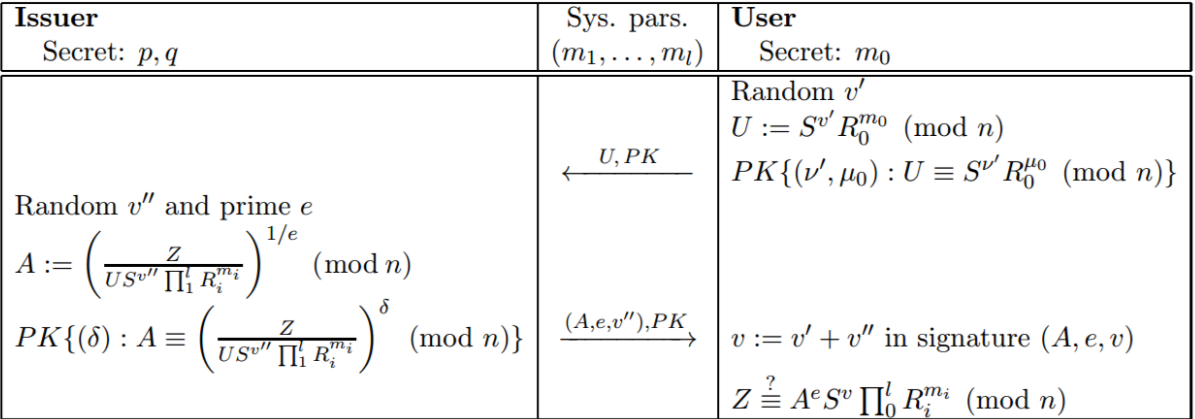
\includegraphics[width=\linewidth]{gfx/issuanceIdemix}
	\end{center}
	\caption{Idemix: firma de credenciales simplificada.}
	\label{fig:issuanceIdemix}
\end{figure}

\hfil


La prueba de conocimiento $P_1$ indica que conocemos un $v'$, primera parte del $v$ final de la firma CL, y un $m_0$, nuestra clave secreta, tales que $U$ se representa como $(v', m_0)$ en la \textit{base} $(S,R_0)$. Utilizando la heurística de Fiat-Shamir, en vez de pedir varios retos al Emisor para conseguir robustez, utilizamos una función de hash junto a un reto $n_1$ del emisor, llamado en inglés \textit{nonce}. La prueba que se envía consiste en el reto obtenido con el hash, y las respuestas a dicho reto.

\begin{algorithm}[$KP\{(v',m_0) : U \equiv S^{v'}R_0^{m_0} \, mod \, n \}(n_1)$]
	\hfil
	
	\begin{enumerate}
		\item Elegir $\tilde{m}_0$ y $\tilde{v}'$ aleatorios.
		\item Calcular $\tilde{U} = S^{\tilde{v}'}\cdot R_0^{\tilde{m}_0} \, mod \, n$.
		\item Reto por heurística Fiat-Shamir: $c = H(U||\tilde{U}||n_1)$.
		\item Respuestas al \textit{reto}: $\hat{v}' = \tilde{v}' + c v'$, $\hat{m}_0 = \tilde{m}_0 + c m_0$.
		\item $P_1 := (c, \hat{v}', \hat{m}_0)$.
	\end{enumerate}
	
\end{algorithm}

\hfil

Para verificar la prueba anterior, por la heurística de Fiat-Shamir (\ref{fiat-shamir-heur}), debemos \textit{recuperar} el valor de $U$ calculado por el Usuario, y comparar los hashes generados.

\begin{algorithm}[Verificar $P_1 := (c, \hat{v}', \hat{m}_0)(n_1)$]
	\hfil
	
	\begin{enumerate}
		\item Calcular $\hat{U} = U^{-c}\cdot S^{\hat{v}'} R_0^{\hat{m}_0} \, mod \, n$.
		\item Aceptar si $c = H(U||\hat{U}||n_1)$.
	\end{enumerate}
	
\end{algorithm}

\hfil


En la prueba de conocimiento del Verificador, demostramos que conocemos la inversa del $e$ de la firma CL, pero sin desvelar su valor, que solo el Emisor, conocedor de $p$ y $q$, puede calcular.

\begin{algorithm}[$KP\{(e^{-1}) : A \equiv \left( \frac{Z}{U\cdot S^{v''}\cdot \prod_{i=1}^{l} R_i^{m_i}} \right)^{e^{-1}} \, mod \, n \}(n_2)$]
	\hfil
	
	Llamemos $Q:=\frac{Z}{U\cdot S^{v''}\cdot \prod_{i=1}^{l} R_i^{m_i}}$.
	\begin{enumerate}
		\item Elegir $r$ aleatorio.
		\item Calcular $\tilde{A} = Q^r \, mod \, n$.
		\item Calcular el reto por Fiat-Shamir $c' = H(Q||A||n_2||\tilde{A})$.
		\item Calcular la respuesta $s_e = r-c'e^{-1}$.
		\item $P_2 := (s_e, c')$.
	\end{enumerate}
	
\end{algorithm}

\hfil

Como antes, \textit{recuperamos} el valor calculado $\tilde{A}$ y comparamos los hashes.

\begin{algorithm}[Verificar $P_2 := (s_e, c')(n_2)$]
	\hfil
	
	\begin{enumerate}
		\item Calcular $\hat{A} = A^{c'+s_e\cdot e} \equiv A^{c'}Q^{s_e} \, mod \, n$.
		\item Aceptar si $c' = H(Q||A||n_2||\hat{A})$.
	\end{enumerate}
	
\end{algorithm}



\subsection{Revelación selectiva de atributos Idemix}

Partiendo de un certificado con la clave secreta $m_0$, los atributos $m_1,\dots,m_l$ y la firma CL $(A,e,v)$, vamos a revelar a un Verificador todos nuestros atributos, excepto los dos primeros, $m_1$ y $m_2$, y por supuesto, tampoco la clave privada $m_0$.

Para esto, primero aleatorizaremos la firma CL como vimos en \ref{CLrandomized} y realizaremos una prueba no interactiva de que conocemos la representación $(m_0,m_1,m_2)$ (\ref{reprKP}) de un cierto valor en una cierta base.

\rule{\textwidth}{1pt}
\begin{algorithm}[Revelación selectiva]
	\hfil
	
	\textit{Conocimiento común}: $n,Z,S,R_0,\dots,R_{l},m_3,\dots,m_l$.
	
	\textit{Conocimiento del Usuario}: $m_0$, su clave secreta, $m_1$ y $m_2$, sus atributos ocultos, $(A,e,v)$ su firma CL.
	
	\hfil
	
	\textit{Protocolo}:
	\begin{enumerate}
		\item V$\rightarrow$ P : valor aleatorio $n_1$.
		
		\item Usuario aleatoriza la firma CL:
		\begin{enumerate}[label*=\arabic*.]
			
			\item $r$ aleatorio, $(A':=AS^{r} (mod\, n),\, e,\, v':=v-er)$
			
		\end{enumerate}
		
		\item Usuario calcula la prueba de conocimiento no interactiva:
		
		$PK\{ (\hat{e},\hat{v}, m_0, m_1, m_2) :  \frac{Z}{\prod_{3}^{l}R_i^{m_i}} \equiv A'^{\hat{e}} S^{\hat{v}}\prod_{i=0}^{2} R_i^{m_i} \, mod \, n  \}(n_1)$
		
		\begin{enumerate}[label*=\arabic*.]
			\item Elige valores aleatorio $\tilde{e}$ y $\tilde{v}'$.
			\item Elige valores aleatorios $\tilde{m}_0$, $\tilde{m}_1$ y $\tilde{m}_2$.
			\item Calcula $\tilde{Z}:=(A')^{\tilde{e}} \left( \prod_{i=0}^3 R_i^{\tilde{m}_i} \right) S^{\tilde{v}'} \, mod \, n $.
			\item Genera el reto por Fiat-Shamir $c:=Hash(A'||\tilde{Z}||n_1)$.
			\item Calcula:
			\subitem $\hat{e}:=\tilde{e}+ce$
			\subitem $\hat{v}':=\tilde{v}+cv'$
			\subitem $\hat{m}_i:=\tilde{m}_i+cm_i$, para $i=0,1,2$.
			\item $P_1:=(c, \hat{e}, \hat{v}', \hat{m}_0, \hat{m}_1, \hat{m}_2)$.			
		\end{enumerate}
		
		\item U $\rightarrow$ V : $A'$ y $P_1$.
		
		\item Verificador comprueba:
		 \begin{enumerate}[label*=\arabic*.]
		 	\item Calcula $\hat{Z}:= \left( \frac{Z}{\prod_{i=3}^{l} R_i^{m_i}} \right)^{-c} (A')^{\hat{e}} \left( \prod_{i=0}^{3} R_i^{\hat{m}_i} \right)  S^{\hat{v}'} \, mod \, n$.
		 	\item Acepta si $c=Hash(A'||\hat{Z}||n_1)$.
		 \end{enumerate}
		
	\end{enumerate}
	

\end{algorithm}
\rule{\textwidth}{1pt}


Tras la ejecución del protocolo anterior, el Verificador conoce algunos de nuestros atributos, y una prueba de que el Emisor nos los firmó, junto a nuestra clave secreta, $m_0$, y otros atributos que hemos ocultado. El Verificador tampoco conoce la firma CL original $(A,e,v)$, sólo $A'$ de la firma aleatorizada, y dos testigos, $\hat{e}$ y $\hat{v}'$ de la misma firma aleatorizada.

Un ejemplo cercano de uso de este protocolo podría ser las encuestas anónimas de asignaturas. Actualmente, si queremos asegurar al alumno que la encuesta es totalmente anónima, sin repercusiones, debemos dejarla \textit{abierta}, pudiendo cualquier persona rellenarla. Si queremos asegurar que sólo los alumnos matriculados puedan acceder a la encuesta, tendrían que iniciar sesión con su correo electrónico, y que confíen en que nadie accederá a sus comentarios.

Con un certificado Idemix, un atributo podría ser ``Alumno de la asignatura X'', otro sus datos de identificación. La Universidad firmó su certificado, que puede llevar en la tarjeta inteligente, por lo que disponemos de una firma CL. Al iniciar sesión en la encuesta, bastaría con mostrar que se es alumno de la asignatura, y generar la prueba no interactiva de que posee un certificado firmado por la Universidad. Sólo los verdaderos alumnos podrán acceder, y ningún registro puede relacionar una opinión con su autor.

Otras soluciones criptográficas tradicionales sólo se preocupaban de proteger la transmisión, que el mensaje no pudiera ser interceptado. Con las pruebas de conocimiento cero hemos conseguido protegernos ante un interlocutor en quien no confiamos.



% TODO: ZKP en multiparty computation: Idemix issuance

%\section{Pruebas de conocimiento cero en criptomonedas}
% O blockchain

% No dependes de los peers para asegurar tu privacidad, ni de una tercera entidad, ni de aplicar otras técnicas sobrela tecnología blockchain, las propias operaciones criptográficas aseguran la privacidad.

% Basecoin <-> Zerocoin : breaks link between new and original Basecoin

% Zerocoin := proof that you owned a Basecoin and made it unspendable
% Miners verify the proofs
% ZKP{ (m) : c==H(m) }  ;  ZKP{ (m) : c1==H(m) OR c2==H(m) OR c3==H(m) }


% Double spending: 
% Obtienes zerocoin: gastas un Basecoin por un zerocoin identificado por H(S,r), S y r secretos.
% ZKP{ (r) : H(S,r) == alguno de los zerocoins en la cadena } + verificar S no gastado antes (S se hace público, r se mantiene secreto).
% Al gastar el zerocoin, no se sabe a cual de los hashes era igual, como todos valen igual, se toma uno cualquiera

% N número de zerocoins en la cadena: tamaño de la prueba es logarítmico respecto N


% Zerocash: zerocoin sin Basecoin, y más eficiente
% No va y vuelve de basecoin a zerocoin, se puede trabajar todo el rato en zerocash
% All transactions are zerocoin
% Splitting and merging are supported. Put transaction value inside the envelope.
% Ledger merely records existence of transactions.
%\cleardoublepage

%\include{multiToC} % <--- just debug stuff, ignore for your documents
% ********************************************************************
% Backmatter
%*******************************************************
\appendix
%\renewcommand{\thechapter}{\alph{chapter}}
\cleardoublepage
\part*{Anexo}
%************************************************
\chapter{Implementaciones}\label{ch:implementaciones} 
%************************************************

?

Implementaciones de símbolos, raíz discreta, simulador de ZKP con QR, ...
%********************************************************************
% Other Stuff in the Back
%*******************************************************
\cleardoublepage%********************************************************************
% Bibliography
%*******************************************************
% work-around to have small caps also here in the headline
\manualmark
\markboth{\spacedlowsmallcaps{\bibname}}{\spacedlowsmallcaps{\bibname}} % work-around to have small caps also
%\phantomsection 
\refstepcounter{dummy}
\addtocontents{toc}{\protect\vspace{\beforebibskip}} % to have the bib a bit from the rest in the toc
\addcontentsline{toc}{chapter}{\tocEntry{\bibname}}
\label{app:bibliography}
\printbibliography


%\cleardoublepage\pagestyle{empty}

\hfill

\vfill


\pdfbookmark[0]{Colophon}{colophon}
\section*{Colophon}
This document was typeset using the typographical look-and-feel \texttt{classicthesis} developed by Andr\'e Miede. 
The style was inspired by Robert Bringhurst's seminal book on typography ``\emph{The Elements of Typographic Style}''. 
\texttt{classicthesis} is available for both \LaTeX\ and \mLyX: 
\begin{center}
\url{https://bitbucket.org/amiede/classicthesis/}
\end{center}
Happy users of \texttt{classicthesis} usually send a real postcard to the author, a collection of postcards received so far is featured here: 
\begin{center}
\url{http://postcards.miede.de/}
\end{center}
 
\bigskip

\noindent\finalVersionString

%Hermann Zapf's \emph{Palatino} and \emph{Euler} type faces (Type~1 PostScript fonts \emph{URW
%Palladio L} and \emph{FPL}) are used. The ``typewriter'' text is typeset in \emph{Bera Mono}, 
%originally developed by Bitstream, Inc. as ``Bitstream Vera''. (Type~1 PostScript fonts were made 
%available by Malte Rosenau and
%Ulrich Dirr.)

%\paragraph{note:} The custom size of the textblock was calculated
%using the directions given by Mr. Bringhurst (pages 26--29 and
%175/176). 10~pt Palatino needs  133.21~pt for the string
%``abcdefghijklmnopqrstuvwxyz''. This yields a good line length between
%24--26~pc (288--312~pt). Using a ``\emph{double square textblock}''
%with a 1:2 ratio this results in a textblock of 312:624~pt (which
%includes the headline in this design). A good alternative would be the
%``\emph{golden section textblock}'' with a ratio of 1:1.62, here
%312:505.44~pt. For comparison, \texttt{DIV9} of the \texttt{typearea}
%package results in a line length of 389~pt (32.4~pc), which is by far
%too long. However, this information will only be of interest for
%hardcore pseudo-typographers like me.%
%
%To make your own calculations, use the following commands and look up
%the corresponding lengths in the book:
%\begin{verbatim}
%    \settowidth{\abcd}{abcdefghijklmnopqrstuvwxyz}
%    \the\abcd\ % prints the value of the length
%\end{verbatim}
%Please see the file \texttt{classicthesis.sty} for some precalculated 
%values for Palatino and Minion.
%
%    \settowidth{\abcd}{abcdefghijklmnopqrstuvwxyz}
%    \the\abcd\ % prints the value of the length





% ********************************************************************
% Game Over: Restore, Restart, or Quit?
%*******************************************************
\end{document}
% ********************************************************************
